	%\documentclass[10pt, draft]{book} % Remove draft for final version
\documentclass[10pt, openany]{book} % Remove draft for final version




\usepackage[table,xcdraw]{xcolor} % % for table, has to be on top so it doesn't clash with others
\usepackage[normalem]{ulem}
\useunder{\uline}{\ul}{}

\usepackage[utf8]{inputenc} % allow direct utf8 input
\usepackage{tabularx} % for rare tables that refuse layout by regular means
\usepackage{watermark} % used for making the thumb indices
\usepackage{tabulary} % allows tables to automatically adjust to line width
\usepackage{parskip} % add empty line between paragraphs
\usepackage{xurl} % break long urls over multiple lines

\usepackage[a5paper]{geometry}
\usepackage{graphicx} % allow figures
\usepackage{fancyhdr} % nice headers and footers
\usepackage[toc,page]{appendix} % allow nice appendix
\usepackage{tabularx} % for rare tables that refuse lay

\usepackage{tikz} % package to create graphic elements, used in chapterstyle.tex

\usepackage[super]{natbib}

\usepackage{chapterbib} % chapterbib allows different bibliographies for each chapter
\usepackage{geometry} % allow difference in margins for some pages

\usepackage{mathtools} % mathematical notations

% To get draft over all pages
%\usepackage{draftwatermark} % to add draft watermark over all pages

\usepackage[font={small}]{caption} % make figure captions small and italic

\usepackage{xcolor} % colour definitions
\usepackage{sectsty} % change header colour


\usepackage{float} % arrange floating of figures

\usepackage{fix-cm} % for large font size


% Important: hyperref should be loaded last
% hidelinks removes the green border around the links
\usepackage[hidelinks]{hyperref} % for label-url style hyperlinks
 % load required packages


\linespread{1.05} % Palatino needs more leading (space between lines)
\renewcommand{\familydefault}{\sfdefault}

\raggedbottom % prevent spreading out paragraphs with lots of whitespace inbetween


% To have draft watermark over the text. Comment when not draft anymore
%\SetWatermarkText{draft v1}
%\SetWatermarkScale{1}
%\SetWatermarkColor[gray]{0.9}


% define colours
\definecolor{DarkBlue}{rgb}{0,0.44705882352,0.69803921568}
\definecolor{LightBlue}{rgb}{0.33725490196,0.70588235294,0.91372549019}
\definecolor{LightOrange}{rgb}{0.90196078431,0.62352941176,0}
\definecolor{DarkOrange}{rgb}{0.83529411764,0.36862745098,0}
\definecolor{Grey}{rgb}{0.50196078431,0.50196078431,0.50196078431}



% use newer pdf version, or it gives warnings with some of my figures that were
% made with newer pdf version
\pdfminorversion=6 % Preamble holds options that are document wide, e.g. chapter style

\begin{document}

\pagestyle{empty}

%\newgeometry{left=-0.50cm,right=-0.50cm,top=0cm,bottom=0cm,centering}
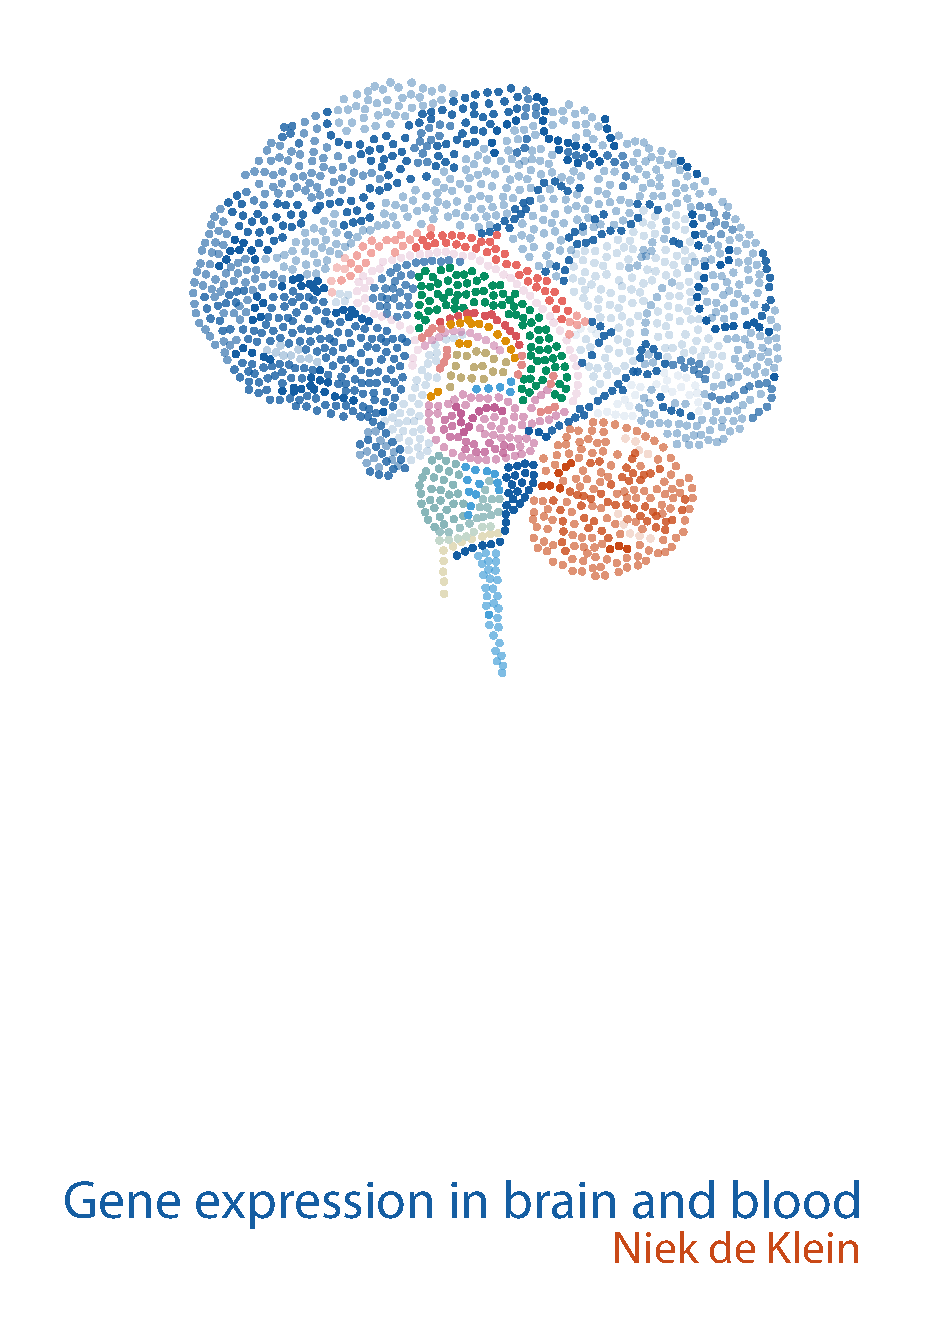
\includegraphics[width=\textwidth,height=0.99999\textheight,keepaspectratio]{img/frontcover}
\restoregeometry
\cleardoublepage


\setcounter{page}{1}

\clearpage
\newgeometry{left=-0.50cm,right=-0.50cm,top=0cm,bottom=0cm,centering}

\restoregeometry
\clearpage

{\small
\noindent
Niek de Klein. \textbf{Title.} Thesis, University of Groningen, with summary in English and Dutch.
\\~\\
The research presented in this thesis was mainly performed at the Department of Genetics, University Medical Center Groningen, University of Groningen, Groningen, the Netherlands. The work in this thesis was financially supported by ...
\\~\\
Printing of this thesis was financially supported by ....
\\~\\
Cover design and layout by ....
The front cover features a.
\\~\\
Printed by ..., ....\\
\\
© 2020 N.P. de Klein. All rights reserved. No part of this book may be reproduced or transmitted in any form or by any means without permission of the author.\\
\\
ISBN: ... \mbox{~~~~~} ISBN (electronic version): ...
}

\begin{figure}[!htbp]
  \centering
  \begin{minipage}[b]{0.19\textwidth}
    \raisebox{0.15\height}{\includegraphics[width=\textwidth]{img/colofon_guide_zw}}
  \end{minipage}
  \hfill
  \begin{minipage}[b]{0.24\textwidth}
    \includegraphics[width=\textwidth]{img/colofon_umcg_zw}
  \end{minipage}
  \hfill
  \begin{minipage}[b]{0.29\textwidth}
    \raisebox{0.4\height}{\includegraphics[width=\textwidth]{img/colofon_rug_zw}}
  \end{minipage}
\end{figure}

\clearpage


\begin{figure}[H]
	
\includegraphics{img/rugr_logonl_zwart_cmyk.eps}
\end{figure}


\huge \textbf{Genetic regulation of gene expression in brain and blood}
\large
\vspace{2.5cm}
\\
\centerline{\textbf{ PhD thesis}}
\normalsize
\vspace{0.5cm}

\centerline{to obtain the degree of PhD at the}
\centerline{University of Groningen}
\centerline{on the authority of the}
\centerline{Rector Magnificus Prof C. Wijmenga}
\centerline{and in accordance with}
\centerline{the decision by the College of Deans.}
\vspace{0.2cm}
\centerline{This thesis will be defended in public on}
\vspace{0.2cm}
\centerline{Monday 13 September 2021 at 11.00 hours }
\vspace{0.5cm}
\centerline{by}
\vspace{0.5cm}
\centerline{\textbf{Niek Peter de Klein}}
\centerline{born on 9 December 1990}
\centerline{in}
\centerline{Velp, the Netherlands}

\newpage
\textbf{Supervisors} \\
Prof. L.H. Franke \\
Prof. C. Wijmenga

\textbf{Assessment Committee} \\
Prof. D. Posthuma \\
Prof. H. Snieder
\\
Prof. P. van der Harst

\newpage
\textbf{Paranymphs} \\
Annique Claringbould
Joana Saldida

\clearpage

\clearpage

\noindent
\textbf{Paranimfen}\\
Annique Claringbould\\
-

\begin{figure}[H]
	
\includegraphics{img/rugr_logonl_zwart_cmyk.eps}
\end{figure}


\huge \textbf{Genetic regulation of gene expression in brain and blood}
\large
\vspace{2.5cm}
\\
\centerline{\textbf{ PhD thesis}}
\normalsize
\vspace{0.5cm}

\centerline{to obtain the degree of PhD at the}
\centerline{University of Groningen}
\centerline{on the authority of the}
\centerline{Rector Magnificus Prof C. Wijmenga}
\centerline{and in accordance with}
\centerline{the decision by the College of Deans.}
\vspace{0.2cm}
\centerline{This thesis will be defended in public on}
\vspace{0.2cm}
\centerline{Monday 13 September 2021 at 11.00 hours }
\vspace{0.5cm}
\centerline{by}
\vspace{0.5cm}
\centerline{\textbf{Niek Peter de Klein}}
\centerline{born on 9 December 1990}
\centerline{in}
\centerline{Velp, the Netherlands}

\newpage
\textbf{Supervisors} \\
Prof. L.H. Franke \\
Prof. C. Wijmenga

\textbf{Assessment Committee} \\
Prof. D. Posthuma \\
Prof. H. Snieder
\\
Prof. P. van der Harst

\newpage
\textbf{Paranymphs} \\
Annique Claringbould
Joana Saldida

\clearpage
\tableofcontents

\newpage
\pagestyle{fancy}

% define \pcolor variable so that colour of chapter can be changed later
\newcommand\pcolor{black}

\fancyhf{}
% tile of chapter above each page
\fancyhead[LE]{\color{\pcolor} \leftmark}
\fancyhead[RO]{\color{\pcolor} \rightmark}
\renewcommand{\headrulewidth}{3pt} % thickness of line

%\chapterfont{\huge\color{Grey}}  % sets colour of chapter

\sectionfont{\color{Grey}}  % sets colour of sections

\subsectionfont{\color{Grey}}  % sets colour of subsections


\renewcommand\pcolor{Grey}
\renewcommand{\headrule}{\hbox to\headwidth{%

		\color{Grey}\leaders\hrule height \headrulewidth\hfill}} % color of title

\fancyfoot[LE,RO]{\thepage}


{ \Large \leftwatermark{

		\put(-76.5,-75){
\includegraphics[scale=0.8]{img/thumbindex/thumbindex_Grey.eps}} 
		\put(-67,-66.5){ {\color{white} 1 }}
		\put(-67,-91.5){ 2 }
		\put(-67,-116.5){ 3 }
		\put(-67,-141.5){ 4 }
		\put(-67,-166.5){ 5 }
		\put(-67,-191.5){ 6 }
	} \rightwatermark{
		\put(346.5,-75){
\includegraphics[scale=0.8]{img/thumbindex/thumbindex_Grey.eps}}  \put(350.5,-66.5){ {\color{white} 1 }}
		\put(350.5,-91.5){ 2 }
		\put(350.5,-116.5){ 3 }
		\put(350.5,-141.5){ 4 }
		\put(350.5,-166.5){ 5 }
		\put(350.5,-191.5){ 6 }
}}

\cleartoleftpage
\makeatletter
\let\savedchap\@makechapterhead
\def\@makechapterhead{\vspace*{-3cm}\savedchap}
\chapter{Introduction}
\let\@makechapterhead\savedchap
\makeatletter
\label{chap:introduction}



\newpage


\noindent


When the first draft of the human genome was released in June of 2000, the then president of the United States, Bill Clinton, told the press that the genome sequence would "revolutionize the diagnosis, prevention, and treatment of most, if not all, human diseases"\cite{collinsHasRevolutionArrived2010}. Without a doubt, the first human genome sequence has revolutionized genomic research. Until that time, genetic studies had mostly focused on rare, monogenic diseases using methods like linkage analysis and Sanger sequencing. At this point there were 2000 genes known that were causal for these rare monogenic diseases. In the 18 years after the first draft of the human genome was completed, there was a four-fold increase in the number of causal genes identified\cite{claussnitzerBriefHistoryHuman2020}. In addition, further developments of computational and DNA sequencing technologies invented or optimized for the human genome project\cite{hoodHumanGenomeProject2013} have helped to bring down the costs of DNA sequencing dramatically, from over \$2 billion for the first human genome to less than \$1000 now. This reduction in cost enabled large projects like the 1000 Genomes project\cite{the1000genomesprojectconsortiumGlobalReferenceHuman2015a} or the Genome of the Netherlands \cite{ fokkemaDutchGenomeDiagnostic2019} and ENCODE\cite{theencodeprojectconsortiumENCODEENCyclopediaDNA2004} to produce maps of sequence variation and to identify functional elements in the human genome. 


The impact of the project was, and still is, enormous and has enabled many advances within genetics and genomics research\cite{chicheBenchtobedsideReviewFulfilling2002} and in identification of new disease genes and has helped to improve genetic diagnosis\cite{claussnitzerBriefHistoryHuman2020}. However, this has only led to treatment in a limited number of cases. Even though diagnosis of genetic disorders has improved, genetic testing is still unable to find the causal genes and variants in the majority of cases\cite{diemenRapidTargetedGenomics2017}. Genetic tests are now successfully used for preventative care of monogenic disorders, such as preventative mastectomies or extra surveillance for BRCA1/2 carriers \cite{heemskerk-gerritsenSurvivalBilateralRiskreducing2019}, but for complex disorders, where many variants have a small effect as opposed to one or a few variants having a large effect, this is still difficult\cite{claussnitzerBriefHistoryHuman2020}. 


Despite the fact that the past 20 years have been full of incredible advances in genomics and genetics research, we are not yet close to the prevention and treatment of most human diseases. Still, there are many ways in which the field of genetics can assist in improving clinical outcome for rare and complex disorders. Currently, there are public-private partnerships under way that will help better our understanding of genotype-phenotype relationships\cite{HomepageInternationalCommon}, provide large data resources for researchers\cite{fingennFinnGenDocumentationR32020,sudlowUKBiobankOpen2015}, and assist in drug target identification\cite{carvalho-silvaOpenTargetsPlatform2019}. Improvements in polygenic risk scores will allow prediction of risk for polygenic traits\cite{natarajanpradeepPolygenicRiskScore2017, kheraGenomewidePolygenicScores2018}, which can help in preventative care for complex disorders. In drug development, the fraction of drug compounds with direct genetic support increases substantially between the preclinical and approved stage (2.0\% versus 8.2\%, respectively\cite{nelsonSupportHumanGenetic2015}), which demonstrates the added benefit of integrating genetic research into the drug development pipeline. 


In this thesis, I address two important factors that are needed if we want to use functional genomics to assist in improving healthcare: (1) insight into the effects of rare variants on gene expression and the genetic architecture of molecular traits and (2) the cell-type- and tissue-context of the genetic effects on molecular traits.


\Needspace{10\baselineskip}
\section{General introduction}

\Needspace{10\baselineskip}
\subsection{Gene regulation through genetic variation}

The central dogma of molecular biology states that genes, the genetic information stored in DNA, are transcribed to RNA, which is then translated to a protein\cite{crickCentralDogmaMolecular1970}. Almost every process in cells is then regulated by these proteins. They act as transcription factors (regulators of gene activity), antibodies (binding to specific foreign particles), enzymes (enablers of many chemical reactions), messengers, and structural components, as well as having roles in transport or storage\cite{uzmanMolecularBiologyCell2003}. However, exceptions to this dogma exist: there are many genes for which the RNA transcript does not get translated to a protein, yet these non-coding genes are often involved in regulating the activity of genes\cite{shabalinaMammalianTranscriptomeFunction2004}. 


The DNA that contains the genetic information consists of about 6.4 billion nucleotide bases divided over 23 chromosome pairs. When comparing a typical human genome sequence to the sequence of the reference human genome, about 4.1 to 5 million sites will be different ($<$ 0.1\%). Most often, these differences are either a difference of a single nucleotide or the insertion or deletion of a single base\cite{the1000genomesprojectconsortiumGlobalReferenceHuman2015a}. Large deletions, duplications, inversions, and other chromosome changes occur, but the focus of this thesis is on single nucleotide changes and short insertions and deletions. Many of these differences will have no noticeable effect on any observable characteristics (the phenotype). Others will have a subtle effect, e.g. having a very small effect on adult height, of which some can also increase risk for common diseases. A smaller fraction of these variants can have more profound effects on certain phenotypes, for example eye colour. And sometime, other rare variants can cause rare but severe genetic disorders such as cystic fibrosis or Huntington’s disease. 


\Needspace{10\baselineskip}
\subsection{The effects of single nucleotide polymorphisms}

Single Nucleotide Polymorphisms (SNPs), the difference of a single nucleotide base, can affect a gene in multiple ways. A SNP within a gene (coding region) can cause the protein product to be prematurely stopped\cite{deboeverMedicalRelevanceProteintruncating2018} or to fold differently\cite{vihinenTypesEffectsProtein2015}, thus reducing or completely removing its functionality. A SNP can also be located outside of the gene (in a non-coding region), for example in the start site of a gene or in an enhancer region, and thereby affecting gene activity. This effect can be measured by dividing people up in their genotype groups, and measuring their gene expression (\textbf{Figure \ref{introduction_fig1}A}) A SNP at a transcription start site can cause a transcription factor to bind with less affinity, thereby lowering gene activity, which can also lead to disorders (\textbf{Figure \ref{introduction_fig1}B}). One example of this is the Pierre Robin sequence, which is caused by changes in non-coding sequences around the SOX9 gene\cite{benkoHighlyConservedNoncoding2009}. However, variation in a non-coding region most often has a smaller effect than mutations in a coding region, and it usually takes multiple non-coding mutations to cause a severe disorder.


\Needspace{10\baselineskip}
\subsection{Genetic disorders}

Genetic disorders are often divided in two broad classes: monogenic disorders\cite{heidiRareGeneticDisorders2008} and complex disorders\cite{craigComplexDiseasesResearch2008}. Monogenic disorders are caused by large-effect variants where a SNP in a single gene is enough to cause a disease. Some well-known examples of monogenic disorders are cystic fibrosis\cite{keremIdentificationCysticFibrosis1989}, sickle-cell anaemia\cite{neelInheritanceSickleCell1949}, and Huntington's disease\cite{gusellaPolymorphicDNAMarker1983}. Complex disorders, on the other hand, are characterised by multiple variants, usually in regulatory regions, that affect the expression levels of multiple genes. Each of these complex disease SNPs confer a limited amount of risk for getting the disease. Examples of complex disorders include diabetes mellitus type 2\cite{americandiabetesassociationDiagnosisClassificationDiabetes2007}, Alzheimer's disease\cite{hardyAlzheimerDiseaseAmyloid1992}, and autism\cite{PolygenicTransmissionDisequilibrium}. For monogenic disorders, it is relatively easy to identify the causal variant because they are most often located within genes and either change important amino acids or cause frame shifts. Identifying associated variants for complex disorders is, however, much more difficult because each variant only has a small contribution, and environmental factors can play an important role as well. Once associated variants have been found, the next challenge: to identify the causal variant remains difficult. For common variants often numerous variants exists that are in strong linkage disequilibrium, making it very challenging to pinpoint the true causal variant.


One step towards identifying associated variants is to create resources of genotype‒phenotype relationships that can be easily used by many researchers.\cite{claussnitzerBriefHistoryHuman2020}. Thanks to large collaborative efforts, there are now biobanks with genotype data for more than 100,000 individuals (for example, the UK biobank\cite{sudlowUKBiobankOpen2015}, LifeLines\cite{scholtensCohortProfileLifeLines2015}, FinnGenn\cite{fingennFinnGenDocumentationR32020} and the Estonian Genome Project\cite{leitsaluCohortProfileEstonian2015}). With these large datasets, it is possible to identify which DNA sequence variants are associated with increased or decreased risk for many different (disease) phenotypes at once, by comparing the genotypes of a large number of healthy people with those of a large group of people with a specific disease or other phenotype. These studies are called Genome Wide Association Studies (GWAS), and many of them are now collected in the GWAS Catalog\cite{bunielloNHGRIEBIGWASCatalog2019}, with the 14 July 2020 GWAS Catalog release containing 116,480 variants for 4,467 phenotypes. The question then remains: What are the molecular mechanisms to which these disease-associated genes contribute to disease risk? One way to discern this is by mapping quantitative trait loci\cite{membersofthecomplextraitconsortiumNatureIdentificationQuantitative2003} (QTLs). Quantitative traits can be any measurable phenotype that varies in the human population due to genetics, e.g. height or molecular traits such as gene expression, protein, or methylation levels. A QTL is a locus, a region on the DNA, where variation affects the quantitative trait. Disease-associated SNPs from GWAS studies can be linked to changes in, for example, expression levels, by mapping expression QTLs (eQTLs; \textbf{Figure \ref{introduction_fig1}A}) for all GWAS SNPs.


The effects that genetic variants have on gene expression can be different depending on the tissue (\textbf{Figure \ref{introduction_fig1}C}) and cell type (\textbf{Figure \ref{introduction_fig1}D}), therefore these genotype-phenotype maps have to be made for all tissues. 


\begin{figure}[H]
	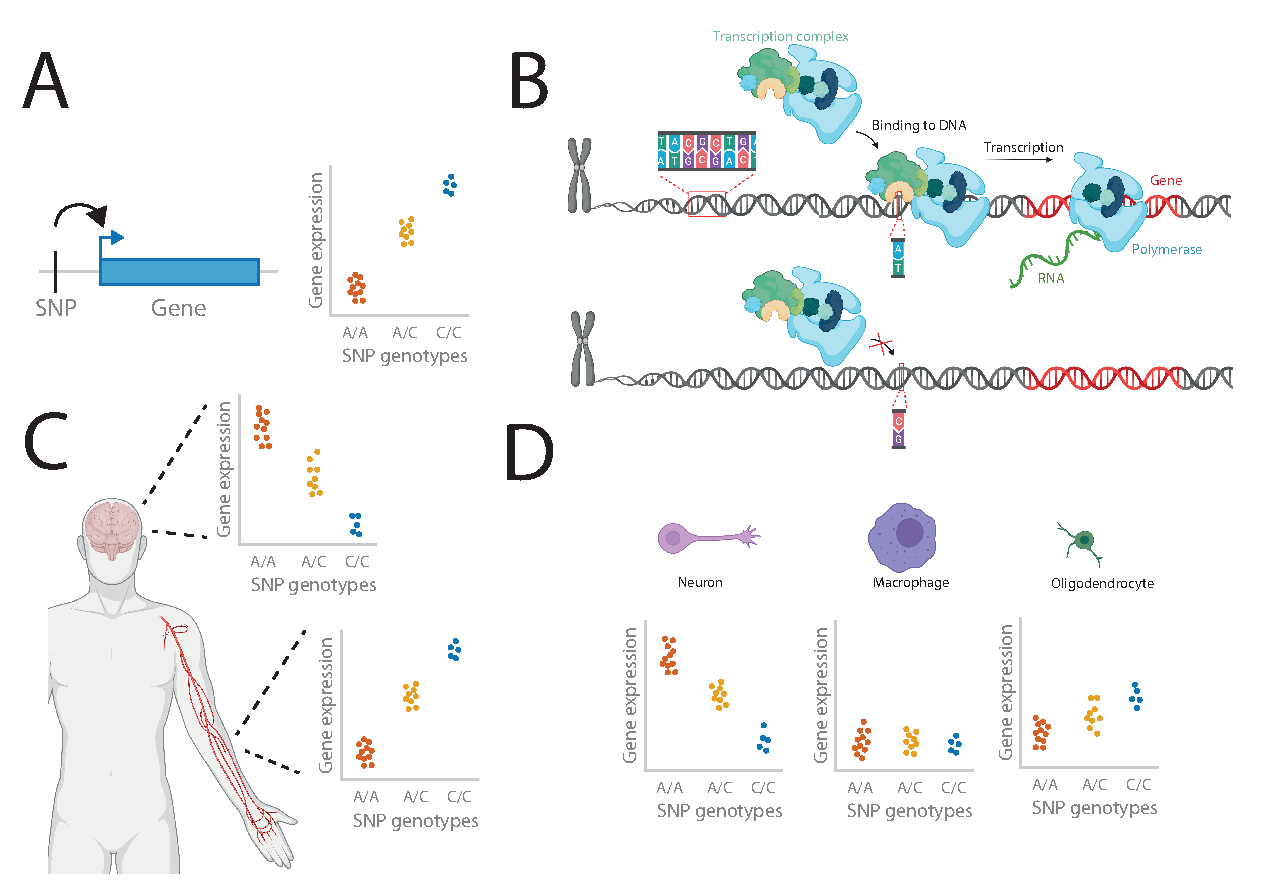
\includegraphics[width=\textwidth]{chapters/chapter1-introduction/img/2021-03-07-fig1.pdf}
	\caption{\textbf{(A) A typical eQTL schematic}. Left:  A position on the DNA that is different between people (single-nucleotide polymorphism, SNP)  affects the expression of a gene. Right: because we have two copies of each chromosome (one from each parent), we have two copies of each DNA position. In this example, the variation of the DNA at this position can be either an adenine (A) or cytosine (C) nucleotide and you can get either from each of your parents. Therefore, people will either have an A on both chromosomes (A/A), an A on one chromosome and a C on the other chromosome (A/C), or a C on both chromosomes (C/C). By comparing the gene expression between these three groups, we can determine if the SNP has an effect on the gene expression. \textbf{(B) An overview of one of the ways in which a SNP might affect gene expression.} A polymerase protein reads the DNA and creates an RNA molecule. The polymerase is recruited to the DNA by the transcription complex, proteins that are bound to the DNA. A change in nucleotides where the transcription complex binds might lower binding affinity. Because of this, the polymerase will transcribe less RNA, and people with the A/C and A/A genotype will have lower expression of the gene as shown in \textbf{panel A}. \textbf{(C) Different genetic effects between tissues.} Because the cellular context, for example the proteins that are present, is different between tissues, it is possible that there is a different effect of the same SNP on the same gene when studying brain or blood samples. \textbf{(D) Different genetic effects between cell types.} Even within cells from the same tissue, such as different cells present in the brain, the effect of a SNP on gene expression can differ.}
	\label{introduction_fig1}
\end{figure}


\Needspace{10\baselineskip}
\section{This thesis}

The aim of this thesis is to get a better understanding of the context in which genetic risk factors influence gene expression levels. In Part 1, we describe the effects of rare variants on gene expression in blood and the genetic architecture of molecular traits. In Part 2, we identify genetic regulation in the context of different cell types in blood and brain.


\Needspace{10\baselineskip}
\subsection{Part 1 - Architecture of molecular traits and rare variant signals}

In Chapter 2, we compared the heritability explained by all the studies included in the GWAS Catalog\cite{bunielloNHGRIEBIGWASCatalog2019} to the heritability explained by expression quantitative trait loci (eQTL) and methylation quantitative trait loci (meQTL) studies. By doing so, we find that the genetic architecture of molecular traits is less polygenic than that of (disease) phenotypes. In chapter 3, we identify the disease categories for which allele-specific expression can be informative for prioritizing putative causal variants.


\Needspace{10\baselineskip}
\subsection{Part 2 - Cell type- and tissue-context of genetic regulation of gene expression}

In chapter 4, we develop two methods. The first predicts the cell count proportions from whole blood samples using gene expression data. The second deconvolutes the cell type‒interacting eQTL effects found in whole blood samples. In chapter 5, we compare the genetic regulation of gene expression in brain and blood and identify which genes affect neurodegenerative and psychiatric disorders. In chapter 6, I discuss how these findings can contribute to improving health care outcomes.



\bibliographystyle{naturemag}

\bibliography{chapters/chapter1-introduction/chapter1-introduction}






%\chapterfont{\color{LightBlue}}  % sets colour of chapter
\sectionfont{\color{LightBlue}}  % sets colour of sections
\subsectionfont{\color{LightBlue}}  % sets colour of subsections

\renewcommand\pcolor{LightBlue}
\renewcommand{\headrule}{\hbox to\headwidth{%
		\color{LightBlue}\leaders\hrule height \headrulewidth\hfill}} % color of title
\fancyfoot[LE,RO]{\thepage}

{ \Large \leftwatermark{
		\put(-67,-66.5){ 1 }
		\put(-76.5,-101){
\includegraphics[scale=0.8]{img/thumbindex/thumbindex_LightBlue.eps}}  
		\put(-67,-91.5){ {\color{white} 2 }}
		\put(-67,-116.5){ 3 }
		\put(-67,-141.5){ 4 }
		\put(-67,-166.5){ 5 }
		\put(-67,-191.5){ 6 }
	} \rightwatermark{
		\put(350.5,-66.5){ 1 }
		\put(350.5,-101){
\includegraphics[scale=0.8]{img/thumbindex/thumbindex_LightBlue.eps}}  
		\put(350.5,-91.5){ {\color{white} 2 }}
		\put(350.5,-116.5){ 3 }
		\put(350.5,-141.5){ 4 }
		\put(350.5,-166.5){ 5 }
		\put(350.5,-191.5){ 6 }
}}

\chapter[The genetic architecture of molecular traits]{The genetic architecture of molecular traits}
\chaptermark{}
\label{chap:chapter2-genetic-architecture}

\hfill \underline{Current Opinion in Systems Biology.} 2017 Feb 16; Volume 1: p25-31.

\hfill DOI: \href{https://doi.org/10.1016/j.coisb.2017.01.002}{j.coisb.2017.01.002}


\noindent
\\
\\
Annique Claringbould\textsuperscript{1,*}, Niek de Klein\textsuperscript{1,*}, Lude Franke\textsuperscript{1,§}
\\
\\
\noindent
1 University of Groningen, University Medical Centre Groningen, Department of Genetics, Antonius Deusinglaan 1, 9713 AV, Groningen, The Netherlands\\
* Equal contribution\\
§ Corresponding author: lude@ludesign.nl
\\
\\
\noindent
published: 6 March 2017.



\section*{Abstract}

Most diseases have both an environmental and genetic component. Although many diseases are strongly heritable, individual genetic variants typically confer only a small effect on disease, and thus these diseases are strongly polygenic. Paradoxically, molecular traits, such as gene expression, methylation, protein or metabolite levels, typically have a lower heritability, but sometimes individual genetic variants show much higher effect sizes on these traits. In this review we discuss the genetic architecture of these molecular traits, and contrast this to the genetic architecture of complex diseases, and provide explanations why strong effects of individual genetic variants on molecular traits do not necessarily need to translate into increased risk of disease.
\\
\\
\begin{figure}[h!]
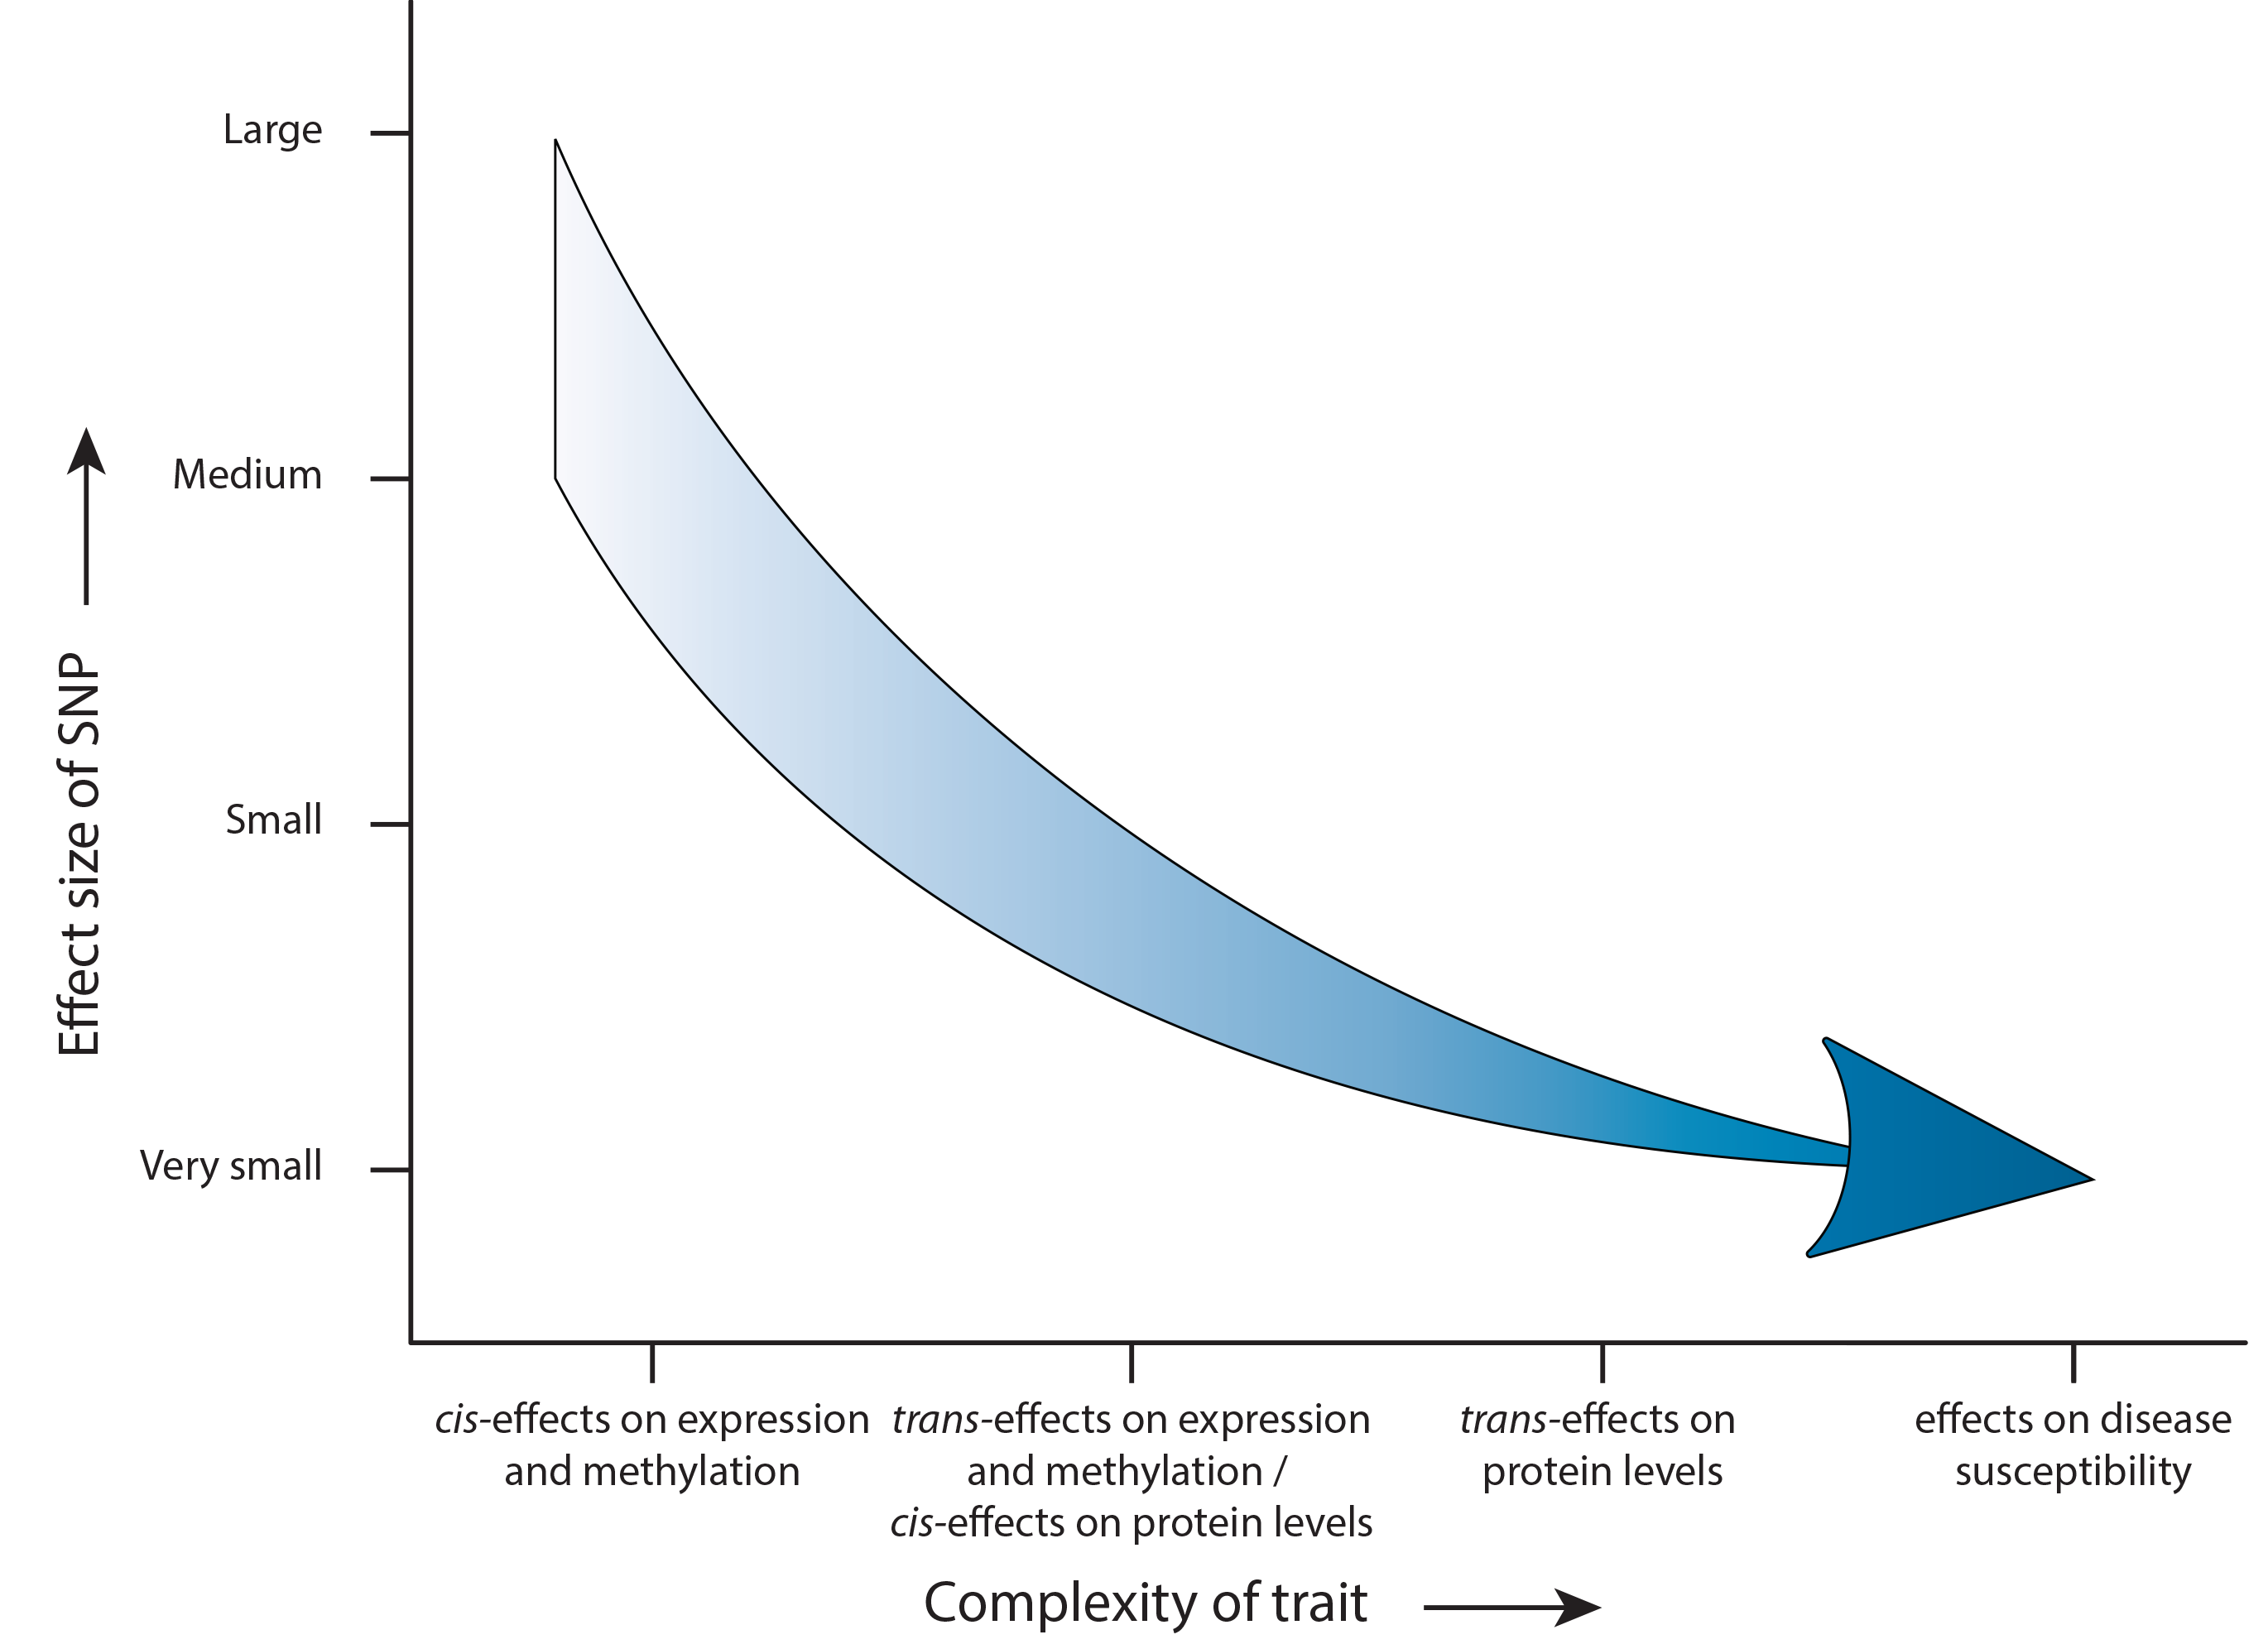
\includegraphics[scale=0.1]{chapters/chapter2-genetic-architecture/img/AbstractFigureCorrectSizeWhite}
\caption{Graphical abstract}
\end{figure}


\section{Introduction}

Since most diseases, phenotypes, and molecular traits are heritable, their genetic architecture is a long-standing question. Are most phenotypes caused by a limited number of large effect variants, or are they due to many variants that each have a small effect? In this review, we compare detected effect size and allele frequencies of associated variants from genome-wide association studies (GWAS) on complex traits and diseases with results from expression- and methylation quantitative trait locus (eQTL and meQTL) studies.

\section{Genetic architecture of common disease: few large effects}
Over the last few years, GWAS have shown that associated variants typically only explain a small proportion of the disease variation seen in the majority of common diseases, despite a few examples of common variants with a large effect being found for immune-related traits, particularly in the HLA-region \cite{dalyHLAB5701Genotype2009}. Currently, variants with an odds ratio (OR) $>$ 10 are considered ‘highly unusual’ \cite{mccarthyGenomewideAssociationStudies2008}. These observations led to an extensive debate about the genetic architecture of complex diseases \cite{mccarthyGenomewideAssociationStudies2008,hansenEvolutionGeneticArchitecture2006,devlinGeneticArchitectureAutism2012,lohContrastingGeneticArchitectures2015,fuchsbergerGeneticArchitectureType2016}, including issues like the number, frequency and effect size of associated genetic variants, as well as the degree of shared genetic background with other traits \cite{mackayGeneticArchitectureQuantitative2001}. For complex diseases the architecture is by no means uniform: the number of genes and their effect sizes differ widely \cite{lohContrastingGeneticArchitectures2015,fuchsbergerGeneticArchitectureType2016,HiddenComplexityMendelian,rheenenGenomewideAssociationAnalyses2016}. However, there is evidence for a shared genetic basis among many diseases \cite{zhernakovaDetectingSharedPathogenesis2009,pickrellDetectionInterpretationShared2016,shiContrastingGeneticArchitecture2016}, and the genetic architecture of most complex disease seems to be highly polygenic.

A much cited interpretation of the overall genetic architecture of diseases places genetic variants in five different groups, based on their allele frequency and effect size or penetrance (\textbf{Figure 1A}, adapted from \cite{mccarthyGenomewideAssociationStudies2008,manolioFindingMissingHeritability2009}). In this representation, complex diseases are characterized by many common genetic variants with small effect sizes, whereas Mendelian diseases are caused by rare variants with large effects. Subsequently, methods were developed that can infer the variance explained by using all directly genotyped SNPs, including those that do not attain genome-wide significance. For complex phenotypes such as height it was established that a considerable proportion of the heritability could be explained by common SNPs, suggesting a highly polygenic genetic architecture \cite{yangCommonSNPsExplain2010}.

\begin{figure}[H]
	\includegraphics[scale=0.3]{chapters/chapter2-genetic-architecture/img/Figure1.png}
	\caption{\footnotesize \textbf{(A)} Proposed genetic architecture of diseases, adapted from Refs. 2, 13. \textbf{(B)} Minor allele frequency (MAF) set out against odds ratio (OR) of genome-wide significant GWAS SNPs. The data is downloaded from the GWAS catalog (Supplementary Note 1). Histograms on the right and at the top indicate the frequency distribution of the SNPs, the dot size indicates the total sample size of the GWAS, and the color represents the year of publication. Rare and intermediate frequency variants (MAF < 0.1) have a higher OR on average. \textbf{(C)} MAF against variance explained (R2) of \emph{cis} expression quantitative trait locus (eQTL) SNPs. Light blue SNPs are from the GEUVADIS consortium (N = 373), dark blue SNPs from the BIOS consortium (N = 2116) (Supplementary Note 2). The plots on the top and right of the figure illustrate the density distribution of SNPs from both cohorts. Despite different sample sizes, the distribution of the \emph{cis} eQTL SNPs is similar for both cohorts. \textbf{(D)} MAF against variance explained (R2) of \emph{cis} and \emph{trans} methylation quantitative trait locus (eQTL) SNPs. Dark blue SNPs are \emph{cis} meQTLs and light blue SNPs are \emph{trans} meQTLs (Supplementary Note 3). Histograms on the right and at the top indicate the frequency distribution of the SNPs. Common SNPs often have large effect sizes, and \emph{trans} effects explain much less methylation variation on average.}
\end{figure}

Indeed, an inventory of the binary traits in the GWAS Catalog (v1.01, r2016-06-12, p $<$ 5x10-8, Supplementary Note 1) reveals that most identified SNPs are common (minor allele frequency (MAF) $>$ 0.1) and have small effect sizes (OR between 1.0 and 1.2, figure 1B). The expectation was that by increasing sample sizes, GWAS would also allow for finding the intermediate frequency variants (0.005 $<$ MAF < 0.1) with larger effects on disease. However, even very large studies have not yet been able to identify many of these hypothesized large effect variants \cite{fuchsbergerGeneticArchitectureType2016} (\textbf{Figure 1B}), while recent studies show that they can be more successfully detected by whole-genome sequencing \cite{del-aguilaAlzheimerDiseaseRare2015,walterUK10KProjectIdentifies2015}.

\section{Genetic architecture of molecular traits}
Surprisingly, the genetic architecture of complex phenotypic (disease) traits differs substantially from the genetic architecture of molecular traits such as gene expression, methylation, or protein levels. Although the genetic architecture of molecular traits can also be polygenic, a single SNP can often explain a considerable part of the heritability compared to disease phenotypes, whereas the heritability of gene expression, methylation or protein levels is typically lower than complex diseases \cite{wrightHeritabilityGenomicsGene2014,poldermanMetaanalysisHeritabilityHuman2015}. 

\section{Large effect-sizes of SNPs affecting molecular traits}
Genetic variation influences the risk of developing a complex disease through several molecular traits such as gene expression \cite{emilssonGeneticsGeneExpression2008} and methylation \cite{conerlyInsightsRoleDNA2010}. Investigating eQTLs \cite{pickrellUnderstandingMechanismsUnderlying2010,lappalainenTranscriptomeGenomeSequencing2013,westraSystematicIdentificationTrans2013,zhernakovaIdentificationContextdependentExpression2017,gibsonExpressionQuantitativeTrait2015} and allele-specific expression (ASE) \cite{deelenCallingGenotypesPublic2015,pirinenAssessingAllelespecificExpression2015,rivasEffectPredictedProteintruncating2015,castelToolsBestPractices2015} can characterize the effect of common and rare genetic variants, respectively, on gene expression. Similarly, intermediate frequency and common SNPs that affect methylation levels at CpG sites can be detected by meQTL mapping \cite{bonderDiseaseVariantsAlter2017}.

Analogous to the genetic architecture of common diseases presented in \textbf{Figure 1B}, the genetic architecture of gene expression and methylation may be represented by plotting the allele frequency of QTLs against their effect size (\textbf{Figure 1C} and \textbf{1D}, \textbf{Supplementary Note 2}). We first compared the proportion of variance explained for \emph{cis}-eQTLs identified in RNA-seq data in blood (BIOS consortium, N=2,116, only SNPs tested with MAF > 0.05) \cite{zhernakovaIdentificationContextdependentExpression2017} and in Epstein-Barr virus-transformed lymphoblastoid cell lines (GEUVADIS consortium, N=373, only SNPs tested with MAF > 0.05) \cite{lappalainenTranscriptomeGenomeSequencing2013}. Comparing the two cohorts indicates that sample size has an impact on the number of identified eQTL SNPs, but not on their effect size (\textbf{Figure 1C}). 

Notably, the effects of many eQTLs and meQTLs are large, especially compared to the degree of heritability of a disease explained by GWAS: some eQTLs explain as much as 80\% of the variation at transcript level (\textbf{Figure 1C}) and many \emph{cis}-meQTLs explain over 70\% of the methylation level variation (\textbf{Figure 1D}). While common GWAS SNPs only rarely have a large effect on the phenotype, the impact of common SNPs on molecular traits can thus be much greater. 
Another observation is that the minor allele frequency distribution of disease variants (\textbf{Figure 1B}) is different from the MAF distribution of both eQTLs and meQTLs (\textbf{Figure 1C} and \textbf{1D}): molecular traits are influenced by variants with on average a lower MAF, as compared to complex traits for which the average MAF is higher.

\section{Many independent SNPs affecting the same molecular trait}
While for many complex diseases many independent associations have so-far been found, the number of independent associations for molecular traits has been studied less well. Conditional analyses (i.e. correction for primary \emph{cis}-eQTLs) can be performed to ascertain whether secondary signals can be identified. Zhernakova et al. (2015) recently performed such an analysis and observed that more than half of the transcripts are governed by more than one \emph{cis}-eQTL effect, suggesting that the genetic architecture of gene expression regulation for most genes is polygenic, similar to complex diseases.

\section{Local and distal effects}
However, these conditional analyses have so-far only identified multiple independent SNPs that are working in \emph{cis}: SNPs most often affect nearby molecular traits in \emph{cis} through mechanisms such as transcription factor binding disruption in regulatory regions or promotor disruption within transcription start sites \cite{brownIntegrativeModelingEQTLs2013}. To identify genetic variants that are distantly located, \emph{trans}-QTL mapping can be conducted. Those \emph{trans} effects are hypothesized to be mediated by multiple \emph{cis} effects and complex downstream regulation on a molecular trait \cite{westraSystematicIdentificationTrans2013,wongInterplayCisTrans2017}, and are identified less frequently (\textbf{Figure 2}), due to severe multiple-testing issues when comparing millions of genetic variants with tens of thousands of molecular traits. So-far the largest QTL studies have observed a \emph{trans}-acting proportion of 4.5\% \cite{westraSystematicIdentificationTrans2013} and 2.4\% \cite{wrightHeritabilityGenomicsGene2014} of total eQTLs, and 3.6\% \cite{bonderDiseaseVariantsAlter2017} and 6.5\% for meQTLs \cite{gauntSystematicIdentificationGenetic2016}. With increasing sample-sizes these estimates will likely go up in the near future, since it has been estimated that \emph{cis}-effects explain only 23\% of the total heritability of gene expression level regulation \cite{wrightHeritabilityGenomicsGene2014}, thus suggesting that distal effects strongly outnumber local effects. However, for both eQTLs and meQTLs, the \emph{cis} effect sizes are on average several times higher than the \emph{trans} effects (\textbf{Figure 1D} and 3A), which is likely due to additional regulation layers between the \emph{cis} effect and the \emph{trans} effect \cite{albertRoleRegulatoryVariation2015}. 

\begin{figure}[H]
	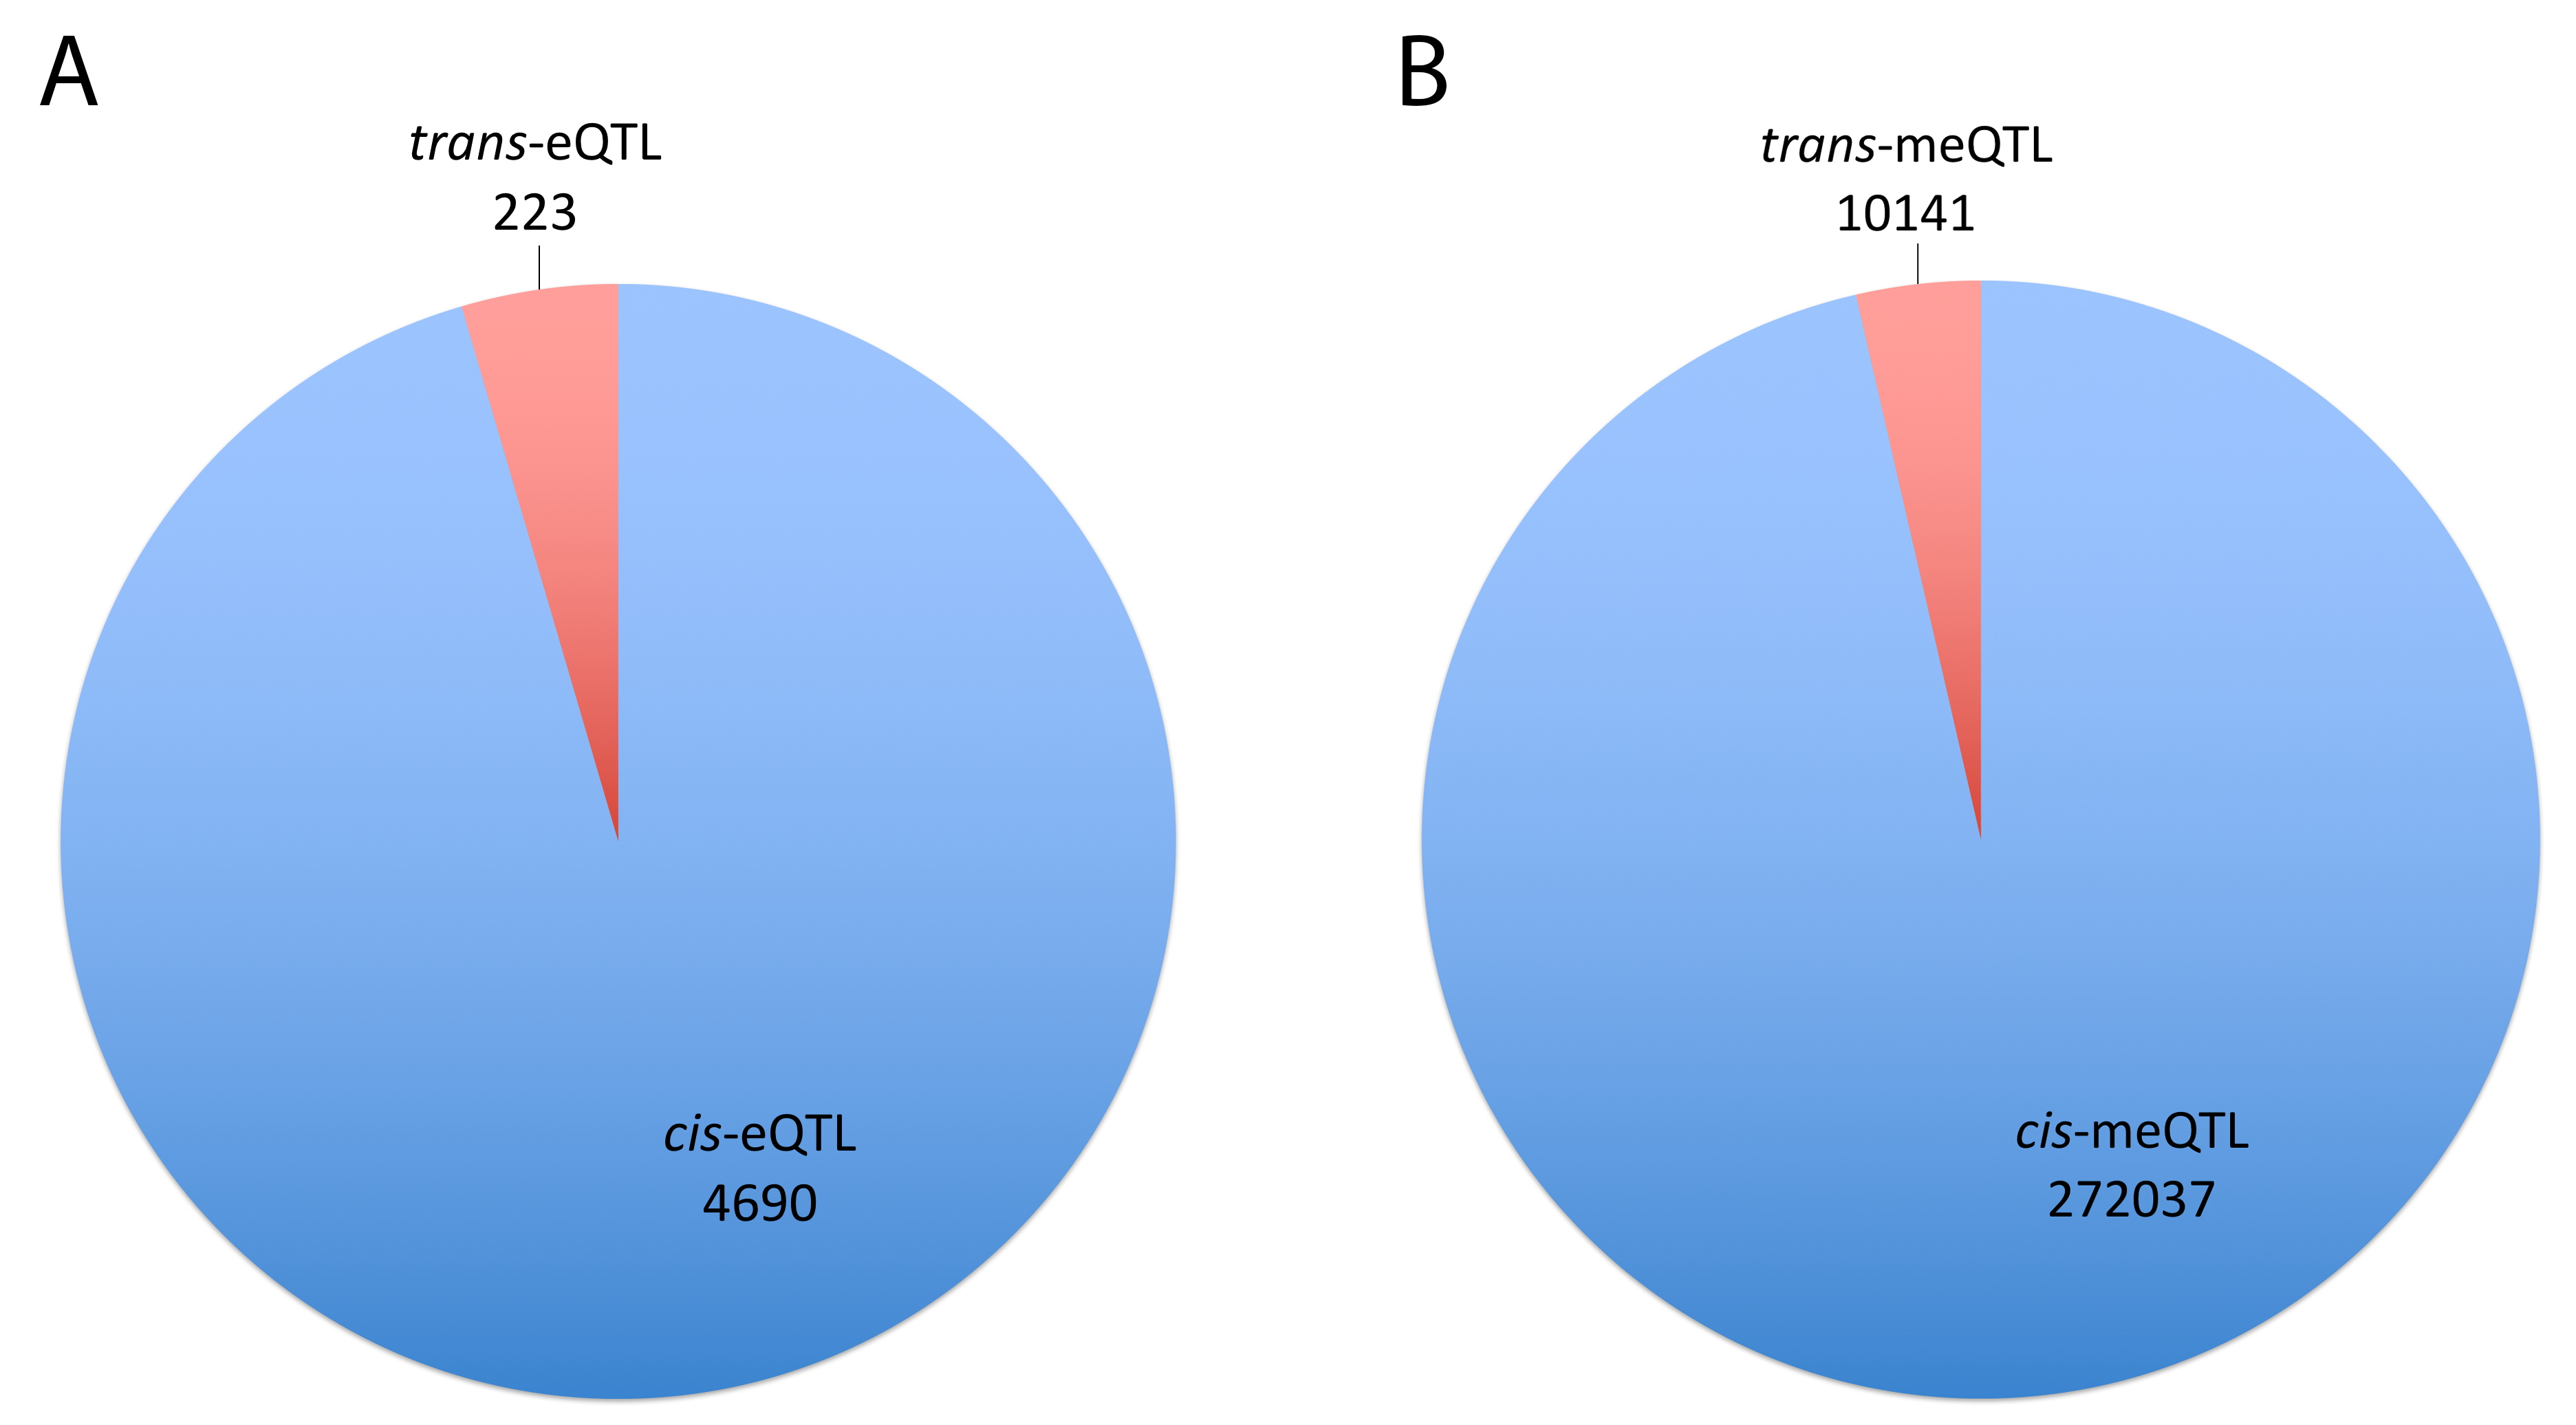
\includegraphics[width=\textwidth]{chapters/chapter2-genetic-architecture/img/Figure2.png}
	\caption{\textbf{(A)}, \textbf{(B)} Pie charts comparing the number of observed eQTLs \textbf{(A)} and meQTLs \textbf{(B)} based on Refs. \cite{zhernakovaIdentificationContextdependentExpression2017,wongInterplayCisTrans2017}. Blue indicates \emph{cis} effects, red are the \emph{trans} effects.}
\end{figure}

\begin{figure}[H]
	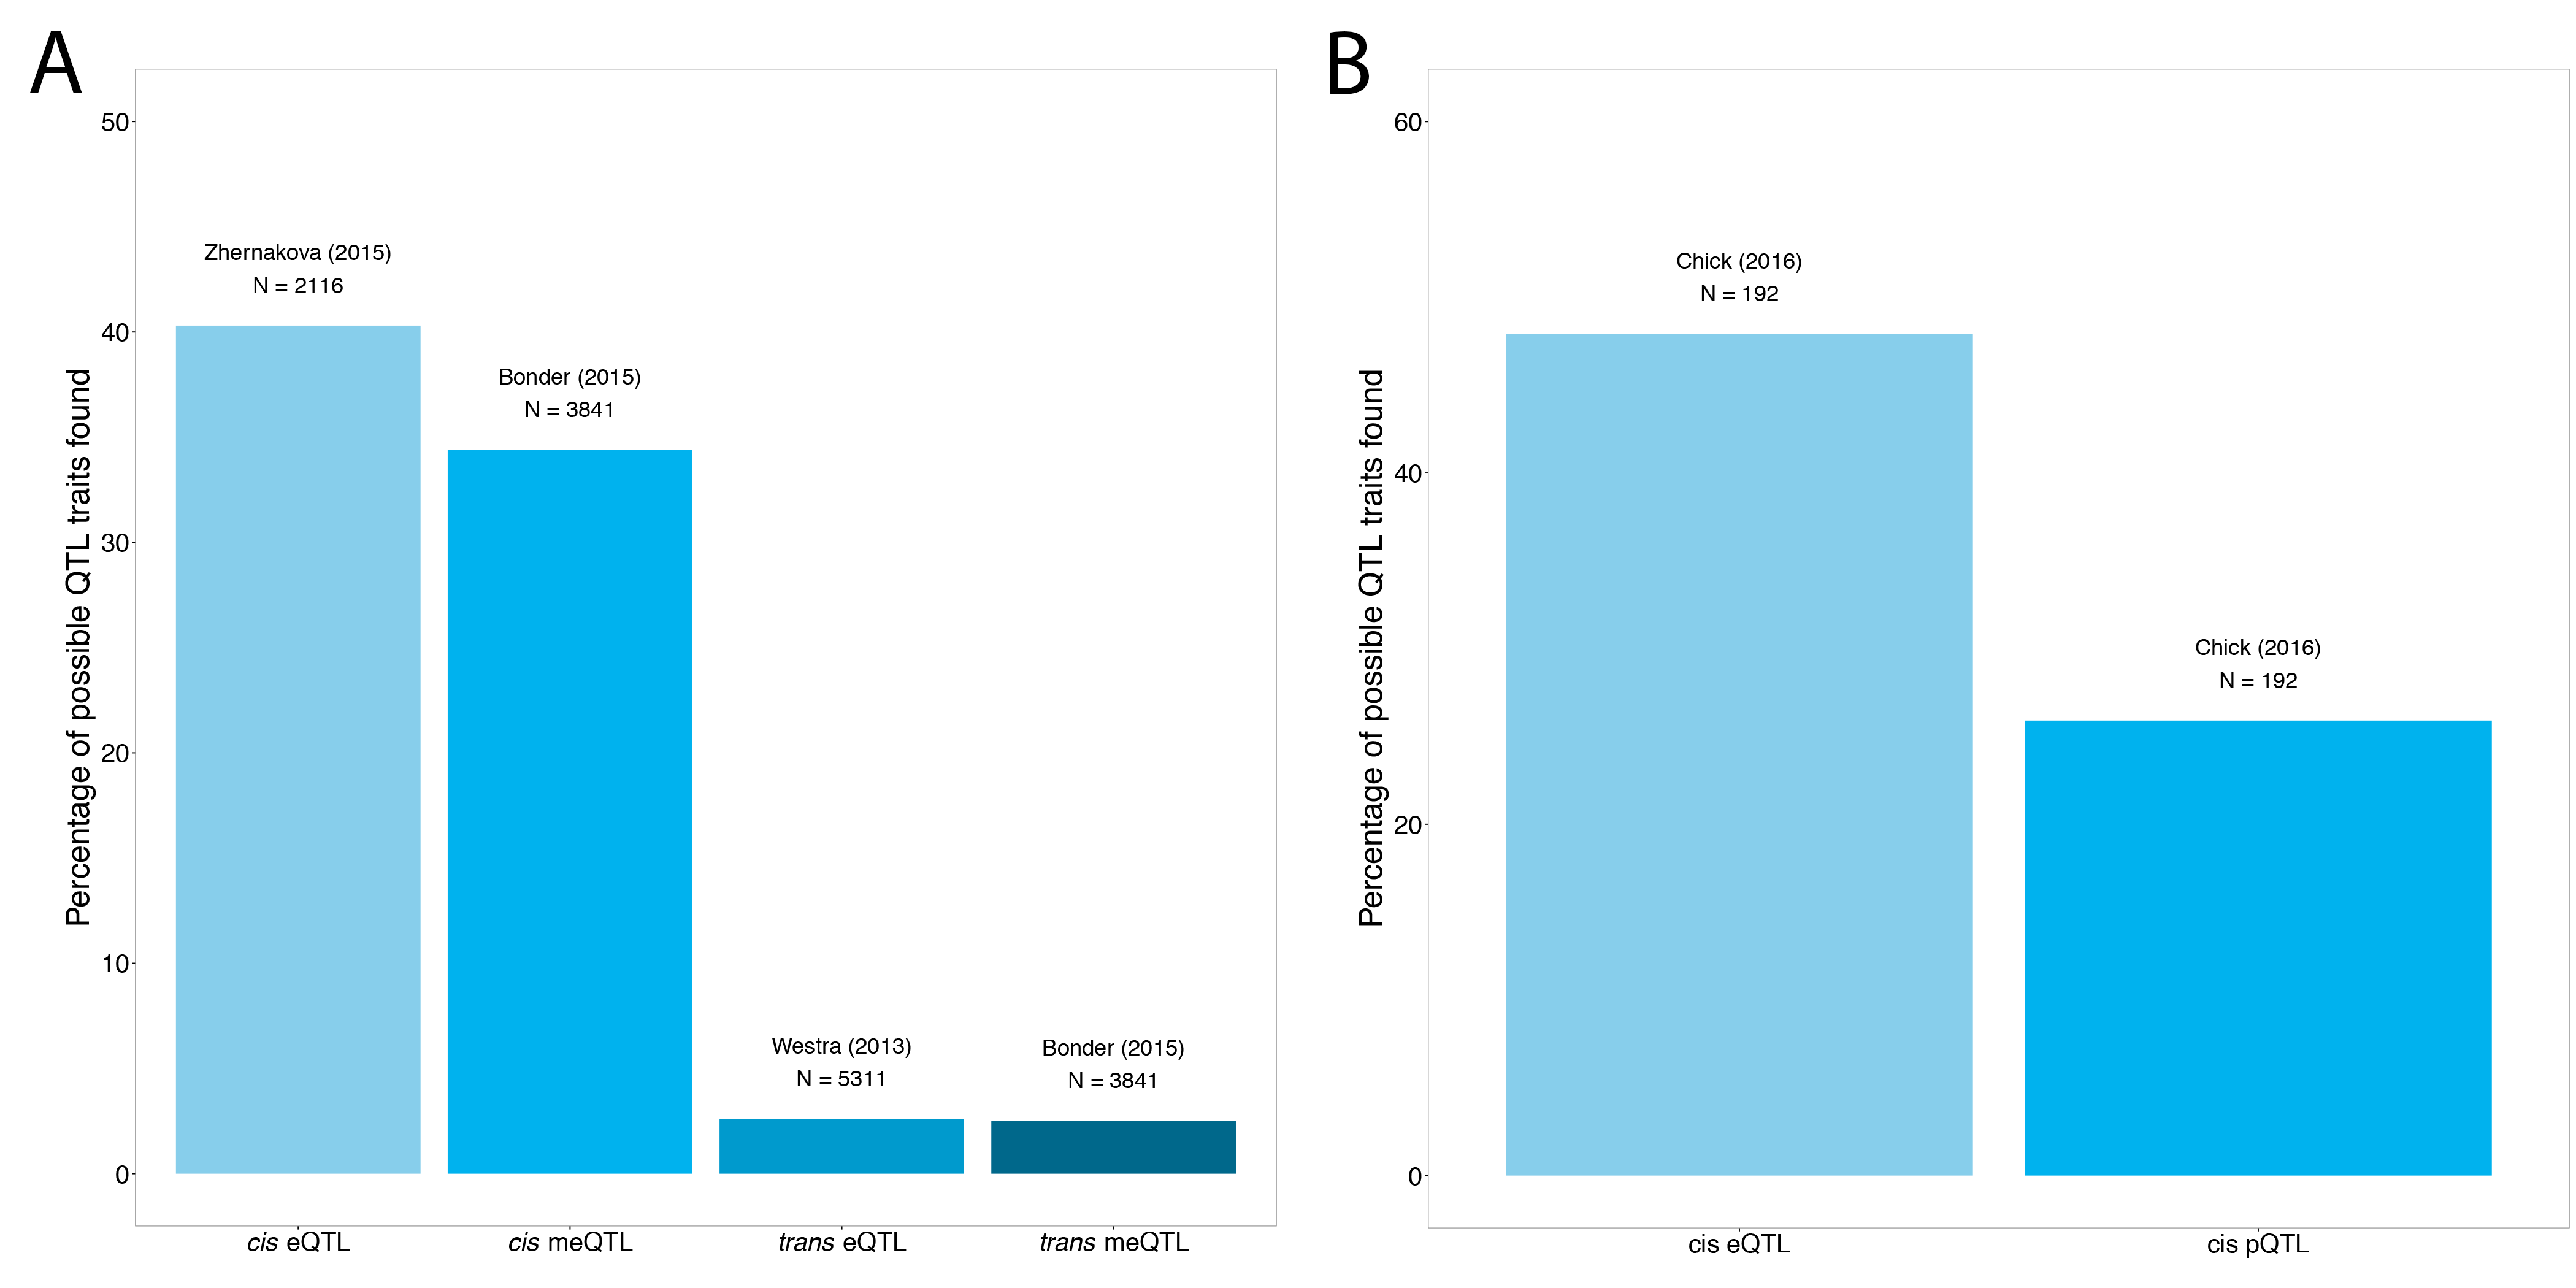
\includegraphics[width=\textwidth]{chapters/chapter2-genetic-architecture/img/Figure3.png}
	\caption{\textbf{(A)} Percentage of total measured SNPs detected as \emph{cis} eQTL, \emph{cis} meQTL, \emph{trans} eQTL and \emph{trans} meQTL SNPs, based on Refs. \cite{zhernakovaIdentificationContextdependentExpression2017,gibsonExpressionQuantitativeTrait2015,wongInterplayCisTrans2017}. Cis effects are identified for a much larger percentage of SNPs compared to \emph{trans} effects. \textbf{(B)} Percentage of total measured SNPs detected as \emph{cis} eQTL, and \emph{cis} protein QTL (pQTL) SNPs in mice, based on Ref. \cite{GenomeWideMetabolicQTL}. For the same mice and the same number of transcripts and proteins, eQTLs are more often detected than pQTLs.}
\end{figure}

With the current sample-sizes, the percentage of tested genes with a significant QTL is higher for \emph{cis} than for \emph{trans} (\textbf{Figure 3A}). This will undoubtedly change when sample-sizes increase further. However, what can be concluded now is that the proportion of CpG sites that show \emph{trans}-meQTL effects is lower than the proportion of genes with a \emph{trans}-eQTL effect. When accounting for the different numbers of samples in \emph{trans}-eQTL and \emph{trans}-meQTL studies this pictue does not change. This indicates that gene expression levels are more polygenic than methylation levels. 

\section{Cell-type and context-specificity of QTLs}
It should be noted, however, that the effects of genetic variants on molecular traits are highly variable: it is now clear that the effects of genetic variation on gene expression levels can depend strongly on cell type, tissue type, and context, such as stimulations by pathogens \cite{fuUnravelingRegulatoryMechanisms2012,gat-viksDecipheringMolecularCircuits2013,fairfaxInnateImmuneActivity2014,leeCommonGeneticVariants2014,meleHumanTranscriptomeTissues2015}. Indeed, blood \emph{cis}-eQTLs are often inconsistent in other tissues: blood QTLs may be absent in a different tissue, they may have a different effect size, or even show an opposite allelic effect \cite{fuUnravelingRegulatoryMechanisms2012}. This is even more pronounced for \emph{trans}-eQTLs: some \emph{trans}-eQTLs can only be replicated in a specific cell type \cite{westraSystematicIdentificationTrans2013}. Tissue-dependent eQTL effects are enriched in SNPs associated with complex traits \cite{fuUnravelingRegulatoryMechanisms2012}, while the cell-type specific effects identified in the HLA region \cite{fairfaxGeneticsGeneExpression2012} are just one example of how tissue specificity can influence the risk of developing the disease. Surprisingly, \emph{trans}-meQTLs are much more stable across cell types \cite{gutierrez-arcelusTissueSpecificEffectsGenetic2015}: it has been shown that the far majority of whole blood \emph{trans}-meQTLs replicate in lymphocytes \cite{bonderDiseaseVariantsAlter2017}, suggesting that meQTLs are generally very stable. It should be noted though, exceptions exist: there are tissue-specific methylation patterns \cite{lokkDNAMethylomeProfiling2014} and \emph{cis}-meQTLs have been found whose CpG levels show correlations with expression levels of tissue-specific alternatively spliced exons \cite{gutierrez-arcelusTissueSpecificEffectsGenetic2015}.

\section{Genetic architecture of other protein and metabolite levels}
Eventually changes in methylation and particularly gene expression levels due to genetic variation should show downstream consequences. Since gene expression levels are not a direct proxy for protein levels \cite{partsHeritabilityGeneticBasis2014,liuInterdependenceTranscriptProtein2016}, protein quantitative trait loci (pQTLs) can give a more accurate measurement of the effect of SNPs on protein abundance. Interestingly, not all pQTLs overlap with eQTLs, suggesting that multiple mechanisms regulate protein levels \cite{wuVariationGeneticControl2013,liuQuantitativeVariability3422015}. Recent research on mice, measuring genome-wide gene expression and protein levels on the same samples, suggests that distal pQTLs act on protein levels through mediator proteins and post-transcriptional mechanisms, while local pQTL SNPs directly influence the protein level through gene expression regulation \cite{chickDefiningConsequencesGenetic2016}. 

Cytokines are a specific class of proteins: they play an important role in immunological disorders. Cytokine abundances are especially variable in response to pathogens, and they can be mapped to SNPs to find stimulation-induced cytokine quantitative trait loci (cQTLs) \cite{luMappingQuantitativeTrait2011,liInterindividualVariabilityGenetic2016}. While some cQTLs are cytokine-specific, other QTLs are shared among cytokines \cite{liInterindividualVariabilityGenetic2016}.

Likewise, it is possible to detect SNPs that influence nuclear magnetic resonance (NMR)-derived metabolite abundances in urine or plasma \cite{GenomeWideMetabolicQTL,shinAtlasGeneticInfluences2014}. These metabolite quantitative trait loci (mQTLs) show that metabolite levels, like protein levels, are highly heritable, with some variants that have been detected explaining more than 40\% of metabolite level variation \cite{GenomeWideMetabolicQTL}. 

As sample sizes of the metabolite and protein QTL studies are still small, they are difficult to compare to the large-scale eQTL and meQTL studies that have been conducted so-far. Human pQTL studies have detected around 180 pQTLs with a large impact \cite{wuVariationGeneticControl2013}: these signals are the ones most easily detected. However, a recent study in mice pQTLs \cite{chickDefiningConsequencesGenetic2016} showed that fewer pQTLs than eQTLs were detected in liver when using the same mice for both analyses (N=192, FDR < 0.01, \textbf{Figure 3B}). Although mice and humans have different physiologies, the finding suggests that human pQTLs are more difficult to detect due to their smaller average effect size. In the future, human pQTL studies with a larger number of samples as compared to eQTL and meQTL studies are therefore needed in order to identify protein and metabolite QTLs that have smaller effect sizes.


\section{Conclusion}
In contrast to GWAS SNPs, SNPs affecting molecular traits can have a very large effect size. Paradoxically, the twin estimated heritability of expression levels (h2=0.142) \cite{wrightHeritabilityGenomicsGene2014} is lower than the twin estimated heritability of diseases (h2=0.593) \cite{poldermanMetaanalysisHeritabilityHuman2015}. Given the strong effect sizes that are often observed for molecular traits, in contrast to complex traits, this suggests that the genetic architecture of molecular traits is much less polygenic than that of complex diseases. 

However, it remains elusive how SNPs can have such a strong effect on a single molecular trait, while they generally have only a small effect on disease phenotypes. One possibility is that the affected molecular trait does not play such an important role. This would explain why there are common SNPs with high effect sizes. Another scenario is that molecular trait levels are redundant: variability of one trait (e.g. the expression levels of a specific gene) may only become important in the absence of the other trait (e.g. another gene that has the same biological function). Alternatively, changes in levels of a single molecular trait need not have a big effect downstream because many proteins are involved in the regulation of a single gene. The abundance of transcripts regulated by more than one \emph{cis}-eQTL in combination with the considerable number of \emph{trans}-acting effects supports the hypothesis that complex pathways buffer the large variation in molecular traits to result in a small disease-inducing effect.

To our knowledge, except for some allele-specific analyses, few QTL studies have so far looked at the molecular effects of rare variants (MAF < 0.005), which makes it hard to predict what effects these variants will have on molecular traits. However, considering that the intermediate variants show an increase in their effect size compared to common variants, and rare SNPs are under more evolutionary pressure, we would expect some of these rare variants to have a very strong effect on molecular traits.

To better understand disease mechanisms we need to gain a more complete picture of the genetic architecture of molecular traits. If rare variants do show an even larger effect on molecular traits than intermediate or common variants, it is key that QTL studies should investigate them using larger sample sizes, as well as using tools designed to identify the effects from rare SNPs, such as allele-specific analysis. 


\section*{Acknowledgements}
We thank Jackie Senior for editing the final text. This work is supported by a grant from the European Research Counsil (ERC Starting Grant agreement number 637640 ImmRisk) to Lude Franke and an NWO-VIDI grant 917-14374 from the Netherlands Organization for Scientific Research. 

\bibliographystyle{naturemag}
\bibliography{chapters/chapter2-genetic-architecture/chapter2-genetic-architecture}
%
\chapterfont{\huge\color{LightOrange}}  % sets colour of chapter
\sectionfont{\color{LightOrange}}  % sets colour of sections
\subsectionfont{\color{LightOrange}}  % sets colour of subsections

\renewcommand\pcolor{LightOrange}
\renewcommand{\headrule}{\hbox to\headwidth{%
		\color{LightOrange}\leaders\hrule height \headrulewidth\hfill}} % color of title
\fancyfoot[LE,RO]{\thepage}



\cleardoublepage
\makeatletter
\let\savedchap\@makechapterhead
\def\@makechapterhead{\vspace*{-3cm}\savedchap}
\chapter[Imbalanced expression for predicted high-impact, autosomal-dominant variants in a cohort of 3,818 healthy samples]{Imbalanced expression for predicted high-impact, autosomal-dominant variants in a cohort of 3,818 healthy samples}
\chaptermark{}
\let\@makechapterhead\savedchap
\makeatletter
\chaptermark{}

\label{chap:chapter3-ase}


\hfill \underline{bioRxiv} 2020 Sep 20;

\hfill DOI: \href{https://doi.org/10.1101/2020.09.19.300095}{2020.09.19.300095}
\\
\\
Niek de Klein\textsuperscript{*}, Freerk van Dijk\textsuperscript{*}, Patrick Deelen, Carlos G. Urzua, Annique Claringbould\textsuperscript, Urmo Võsa, Joost A.M. Verlouw, Ramin Monajemi, Peter A.C. ‘t Hoen, Richard J. Sinke, BIOS Consortium, Morris A. Swertz and Lude Franke
\\
\\
* These authors contributed equally to this work.

\newpage

{ \Large \leftwatermark{
		\put(-50,-66.5){ 1 }
		\put(-50,-91.5){ 2 }
		\put(-97.5,-126){
\includegraphics[scale=0.8]{img/thumbindex/thumbindex_LightOrange.eps}}  
		\put(-50,-116.5){ {\color{white} 3 }}
		\put(-50,-141.5){ 4 }
		\put(-50,-166.5){ 5 }
		\put(-50,-191.5){ 6 }
	} \rightwatermark{
		\put(388,-66.5){ 1 }
		\put(388,-91.5){ 2 }
		\put(380,-126){
\includegraphics[scale=0.8]{img/thumbindex/thumbindex_LightOrange.eps}}  
		\put(388,-116.5){ {\color{white} 3 }}
		\put(388,-141.5){ 4 }
		\put(388,-166.5){ 5 }
		\put(388,-191.5){ 6 }
}}


\section*{Abstract}
\textbf{Background} One of the growing problems in genome diagnostics is the increasing number of variants that get identified through genetic testing but for which it is unknown what the significance for the disease is (Variants of Unknown Significance - VUS)\cite{hoffman-andrewsKnownUnknownChallenges2018,direstaNextgenerationSequencingApproach2018}. When these variants are observed in patients, clinicians need to be able to determine their relevance for causing the patient’s disease. Here we investigated whether allele-specific expression (ASE) can be used to prioritize disease-relevant VUS and therefore assist diagnostics. In order  to do so, we conducted ASE analysis in RNA-seq data from 3,818 blood samples (part of the the Dutch BIOS biobank consortium), to ascertain how VUS affect gene expression. We compared the effect of VUS variants to variants that are predicted to have a high impact, and variants that are predicted to be pathogenic but are either recessive or autosomal-dominant with low penetrance.


\textbf{Results} For immune and haematological disorders, we observed that 24.7\% of known pathogenic variants from ClinVar show allelic imbalance in blood, as compared to 6.6\% of known benign variants with matching allele frequencies. However, for other types of disorders, ASE information from blood did not distinguish (likely) pathogenic variants from benign variants. Unexpectedly, we identified 5 genes (\textit{ALOX5}, \textit{COMT}, \textit{PRPF8}, \textit{PSTPIP1} and \textit{SH3BP2}) in which seven population-based samples had a predicted high impact, autosomal-dominant variant. For these genes the imbalanced expression of the major allele compensates for the lower expression of the minor allele.


\textbf{Conclusions} Our analysis in a large population-based gene expression cohort reveals examples of high impact, autosomal-dominant variants that are compensated for by imbalanced expression. Additionally, we observed that ASE analyses in blood are informative for predicting pathogenic variants that  are associated with immune and haematological conditions. We have made all our ASE results, including many ASE calls for rare variants (MAF $<$ 1\%), available at \url{https://molgenis15.gcc.rug.nl/}. 

\Needspace{10\baselineskip}
\section{Introduction}
One of the challenges in the diagnosis of genetic disorders is the growing number of Variants of Unknown Significance (VUS)\cite{hoffman-andrewsKnownUnknownChallenges2018,direstaNextgenerationSequencingApproach2018}). As (clinical) exome sequencing becomes more prevalent, new variants are increasingly being identified, but the consequences of these rare variants remain mostly unknown. However, a recent study suggested that rare variants might explain much of the missing heritability\cite{wainschteinRecoveryTraitHeritability2019}. For common variants, genome-wide association studies and expression Quantitative Trait Loci (eQTL) studies\cite{zhernakovaIdentificationContextdependentExpression2017,aguetGeneticEffectsGene2017,vosaUnravelingPolygenicArchitecture2018} are commonly used to identify disease-associated variants and infer their molecular consequences. This has led to the observation that many of these genetic risk factors affect gene expression, indicating that transcriptional consequences are informative for predicting whether a common variant is associated with disease. By further increasing eQTL sample sizes, it is now possible to make such inferences for variants with a minor allele frequency (MAF) of at least 1\%\cite{vosaUnravelingPolygenicArchitecture2018}. However, the power to make inferences for rarer variants remains limited. One way to resolve this is to identify their downstream molecular consequences by studying allele-specific expression (ASE)\cite{bombaImpactRareLowfrequency2017}. Knowledge about rare variants gained using this approach can then aid in interpreting their pathogenicity, which could substantially increase the diagnosis rate of patients\cite{macarthurGuidelinesInvestigatingCausality2014,kremerGeneticDiagnosisMendelian2017}. As such, RNA-Sequencing methods can help prioritize rare variants that show downstream molecular effects and are more likely to cause (rare) disorders.

Here we studied RNA from whole blood for 3,818 unrelated individuals from BIOS, a large Dutch biobank consortium. To identify rare variants, we conducted genotype calling on the RNA-Sequencing data directly. We then studied ASE for 297,656 high quality variants and identified 45,197 variants that show an allelic imbalance. We showed that known pathogenic variants are more likely to show an ASE effect. Furthermore, downstream analyses identified 7 samples carrying high impact, autosomal-dominant variants, which showed strong allelic imbalance.

\Needspace{10\baselineskip}
\section{Results}
\Needspace{10\baselineskip}
\subsection{RNA-Seq data can be used to create high-quality phased genotypes}
We first determined the genotypes for all BIOS samples using RNA-Seq expression data by employing a modified version of the GATK\cite{mckennaGenomeAnalysisToolkit2010} best practices workflow for genotyping (see Methods). After joint genotype calling and filtering out genotypes with low quality, low call rate, or overlap with RNA-editing sites, missing genotype calls were imputed to their most likely genotypes using a backbone of genotyping array-genotypes and genotypes called from RNA-Seq. After quality control (QC), 297,656 SNPs in 9,507 genes were called (\textbf{Supplementary Figure 1A}), and most of these SNPs had a low MAF (mean MAF = 0.036, \textbf{Supplementary Figure 1B}). The number of low MAF SNPs is so high largely due to the limitation of calling genotypes from RNA-Seq data, as genes have to be sufficiently expressed.

\begin{figure}[h!]
	\includegraphics[width=\textwidth]{chapters/chapter3-allele-specific-expression/img/fig1.png}
	\caption{\textbf{Quality of RNA-seq based genotypes for allele specific expression analysis.} A) Allele frequency comparison showing strong correlation between WGS genotypes and RNAseq genotypes for 68,564 SNPs from the same samples. B) The same allele frequency comparison between RNAseq-based genotypes and WGS genotypes for rare variants. C) RNAseq-based genotype switching error after phasing. D) Comparison in allelic effect direction between blood and GTEx whole blood ASE. }
	\label{ase_fig1}
\end{figure}

For 249 samples, whole-genome sequencing (WGS) data was available from the Genome of the Netherlands (GoNL) project\cite{boomsmaGenomeNetherlandsDesign2014}, and we used this data as a gold standard comparison set to assess genotype quality. For genotypes called with our RNA-Seq genotype approach and present in the WGS data (73,422 variants, 78.95\% of GoNL RNA-Seq variants were available in GoNL WGS data), we observed a mean genotype concordance of 98.27\%. Furthermore, the allele frequency (AF) was highly concordant (R2 = 0.99, \textbf{Figure \ref{ase_fig1}A)} and similar at lower frequencies (AF $<$ 0.1: R2 = 0.937, \textbf{Figure \ref{ase_fig1}B}). 

ASE for a gene can only be calculated if there is at least one heterozygous site within that gene. In total, we were able to genotype 9,508 genes in which at least one sample had a heterozygous coding SNP, with a mean of 1,495 samples with at least one heterozygous SNP per gene. Of the genes where we found no samples with a heterozygous genotype, these genes were either not expressed or expressed at very low levels in blood, which prevented determination of the genotype. Overall, per sample genotype data could be derived for 3,650 genes on average (\textbf{Supplementary Figure 2B}). We then used SHAPEIT\cite{oconnellGeneralApproachHaplotype2014} to phase imputed genotypes to haplotypes and to calculate haplotype- and gene-level ASE effects. To determine the quality of the phasing, we again used the 249 samples for which WGS genotypes were available, and which were previously trio-phased with their parents, as the gold standard. In this data 69,752 heterozygous SNPs were called, of which 10,465 (15\%) have at least 1 sample with a switch error. For most SNPs, only 1 or a few samples had a switch error per SNP. Averaged over all SNPs and samples 1.97\% had a switch error (\textbf{Figure \ref{ase_fig1}C}). Together, this shows that the phasing of the RNA-Seq-based genotypes is of high quality, meaning that these data could be used for gene-based ASE.

\Needspace{10\baselineskip}
\subsection{Selection of samples showing strong gene-level ASE effects}
We measured three types of ASE effects: SNP-level ASE over the whole population (for validating ASE results), SNP-level ASE per sample, and gene-level ASE (geneASE). SNP-level ASE over the whole population is calculated by per SNP summing minor counts for all samples and summing major counts for all samples, and subsequently performing a binomial test with an expected p of 0.5. In order to correct for multiple testing, we employed the Benjamini-Hochberg method and considered those SNPs significant when the false discovery rate (FDR) was less than 0.05. GeneASE takes into account the summed haplotype counts for all the heterozygous SNPs that overlap the gene. For geneASE, we determined per gene for all samples separately, whether there is an ASE effect by summing the counts of haplotype A and summing the counts of haplotype B, and subsequently performing a binomial test for every gene on the summed haplotype A and haplotype B count for that sample with expected p = 0.5. In order to correct for multiple-testing we again used the Benjamini-Hochberg method and all samples with an FDR $<$ 0.05 were considered to show a significant ASE effect, yielding a total of 3,611 genes with at least 1 sample that showed geneASE. On average, 50 samples show an ASE effect per gene.

The SNP-level ASE per sample was determined in the same way as the GeneASE, but instead of using haplotype A and haplotype B counts, the SNP minor and major allele counts were used.

\Needspace{10\baselineskip}
\subsection{ASE is replicated in GTEx whole-blood ASE and in eQTLs}
To validate the ASE calls, we compared our SNP-level ASE over the whole population to eQTLs on the same dataset and ASE effects found in LCL cell lines\cite{deelenCallingGenotypesPublic2015} and GTEx\cite{pirinenAssessingAllelespecificExpression2015}. For each SNP for which at least 30 individuals were heterozygous, we summed the read counts overlapping the major allele and those overlapping the minor allele over all samples heterozygous for that SNP. We filtered out SNPs with 0 counts on the minor or major allele and calculated a ratio with -1*(0.5 - (major allele count / total count)), so that a negative ratio means that the minor allele has more reads than the major allele, and a positive ratio means the major allele has more reads than the minor allele. We compared this ratio to the BIOS eQTL z-score, allelic ratio of LCL ASE and allelic ratio of GTEx ASE. 

For the eQTLs, there was an overlap of 4,394 SNPs with False Discovery Rate (FDR) $<$ 0.05 for both the ASE effect and the eQTL effect. Of these overlapping SNPs, 87.5\% had the same direction with a Spearman correlation coefficient of 0.78. For LCL ASEs, 7,901 SNPs overlapped when selecting only those SNPs with at least 30 heterozygous samples that are significant in both datasets (FDR $<$ 0.05), with a 72.2\% allelic concordance and Spearman correlation coefficient of 0.527 (\textbf{Supplementary Figure 4}). As expected, since it is the same tissue, we find the largest ASE overlap with GTEx whole blood. There were 9,117 overlapping SNPs after filtering for FDR $<$ 0.05 and at least 30 samples, these 9,117 SNPs had a Spearman R2 of 0.72 and an allelic concordance of 82.65\% (\textbf{Figure \ref{ase_fig1}}). For other GTEx tissues the Spearman R2 was between 0.6 and 0.68 (\textbf{Supplementary Figure 5}).

\Needspace{10\baselineskip}
\subsection{Rare variants are not enriched for ASE effects}
Rare variants are thought to have a large contribution to disease phenotypes and those that show eQTLs effects usually have higher effect sizes than common variants \cite{claringbouldGeneticArchitectureMolecular2017}, although this can also be explained by power issues. We therefore assessed whether rare variants affect allelic imbalance more often than common variants. To test this, we used the geneASE described to define genes showing ASE and genes not showing ASE, and subsequently counted the number of heterozygous SNVs within the genes for different MAF bins ($<$ 0.1\%, 0.1-1\%, 1-5\%, 5-50\%). We then tested, per sample, whether genes with an allelic imbalance contained more rare variants than genes that did not show an allelic imbalance and found that genes containing common heterozygous variants showed an allelic imbalance more often than genes containing rare variants (\textbf{Supplementary Figure 6}, p $< 1 \times 10^{-300}$). This suggests that although the effects of rare variants might be larger, proportionally rare variants show allelic imbalance less often than common variants. 

\Needspace{10\baselineskip}
\subsection{Known pathogenic variants from the ClinVar and VKGL databases show a high proportion of allelic imbalance}
To investigate if ASE can be used to prioritize likely pathogenic variants, we tested if genes containing pathogenic SNPs show allelic imbalance more often than genes containing benign SNPs. We took the 341,303 variants annotated by the ClinVar database (downloaded 19-02-2019) and selected 63,983 high-confidence variants (criteria provided, multiple submitters, no conflicts). For our 318,782 high-quality genotypes, 2,746 overlapped with these high confidence variants (2,200 benign, 125 pathogenic and 421 VUS). For 162 of these (113 benign, 8 pathogenic and 41 VUS) the gene in which the SNP is located did not have any allelic counts (e.g. because there were no heterozygous individuals with enough reads for this gene). For the remaining 2,584 variants, we compared the fraction of samples that show geneASE (binomial test p-value $<$ 0.05 after Bonferroni correction) between pathogenic variants, VUS and benign variants. For ClinVar-annotated variants, genes that contained pathogenic variants showed allelic imbalance more frequently than genes that contained VUS and benign variants (5.89\%, 2.87\% and 3.01\% respectively, \textbf{Figure \ref{ase_fig2}B})\cite{landrumClinVarImprovingAccess2018}. We observed similar results looking at data from the VKGL data share consortium\cite{fokkemaDutchGenomeDiagnostic2019}, a Dutch variant classification database of annotated variants, where there was more allelic imbalance for pathogenic variants than for benign variants (20.3\% versus 4.9\%, \textbf{Figure \ref{ase_fig2}B}). 

\begin{figure}[h!]
	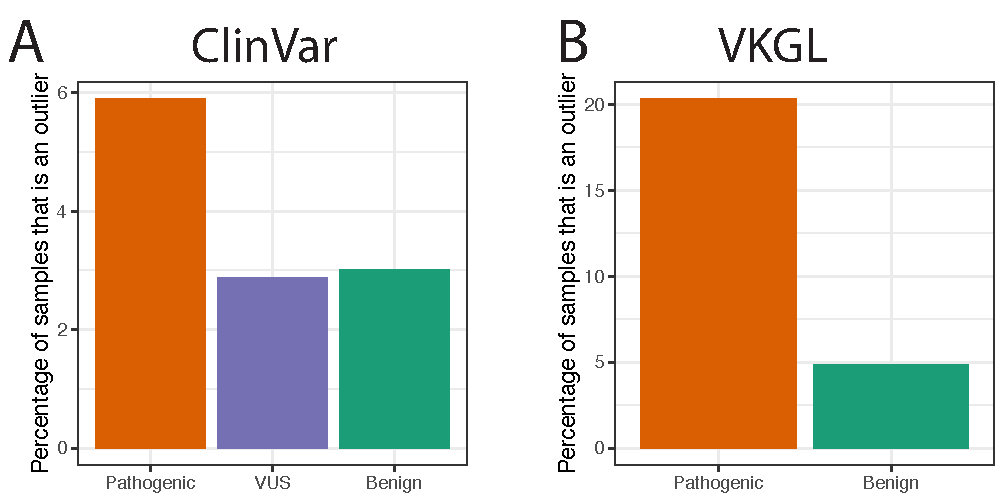
\includegraphics[width=\textwidth]{chapters/chapter3-allele-specific-expression/img/fig2.pdf}
	\caption{\textbf{Comparison of the percentage of variants that show allelic imbalance between ClinVar- and VKGL-annotated variants.} (A) Percentage of samples that show allelic imbalance if they carry a pathogenic, VUS, or benign variant per ClinVar-annotated pathogenicity group. (B) Percentage of samples that show allelic imbalance if they carry a pathogenic, or benign variant per VKGL-annotated pathogenicity group. VKGL is a Dutch variant classification database. }
	\label{ase_fig2}
\end{figure}


We then annotated the genes in which these SNPs are located into different disease categories using the Online Mendelian Inheritance in Men (OMIM) database\cite{hamoshOnlineMendelianInheritance2000} and SnpEff\cite{cingolaniProgramAnnotatingPredicting2012}. For some disease categories, where high-impact variants (as predicted by SnpEff\cite{cingolaniProgramAnnotatingPredicting2012}) are found within genes, the fraction of outlier genes is higher for the high-impact variants than for the benign variants. For example, high impact variants showed higher allelic imbalance than low and moderate impact variants for “allergy/immunology/infectious” diseases, “audiologic/otolaryngologic” diseases, “hematologic” diseases, and dental diseases, while no such difference was seen for other disease categories (\textbf{Figure \ref{ase_fig3}}). This suggests that ASE works better in prioritizing variants when RNA-Seq measurements are taken from disease-relevant tissue. 

\begin{figure}[h!]
	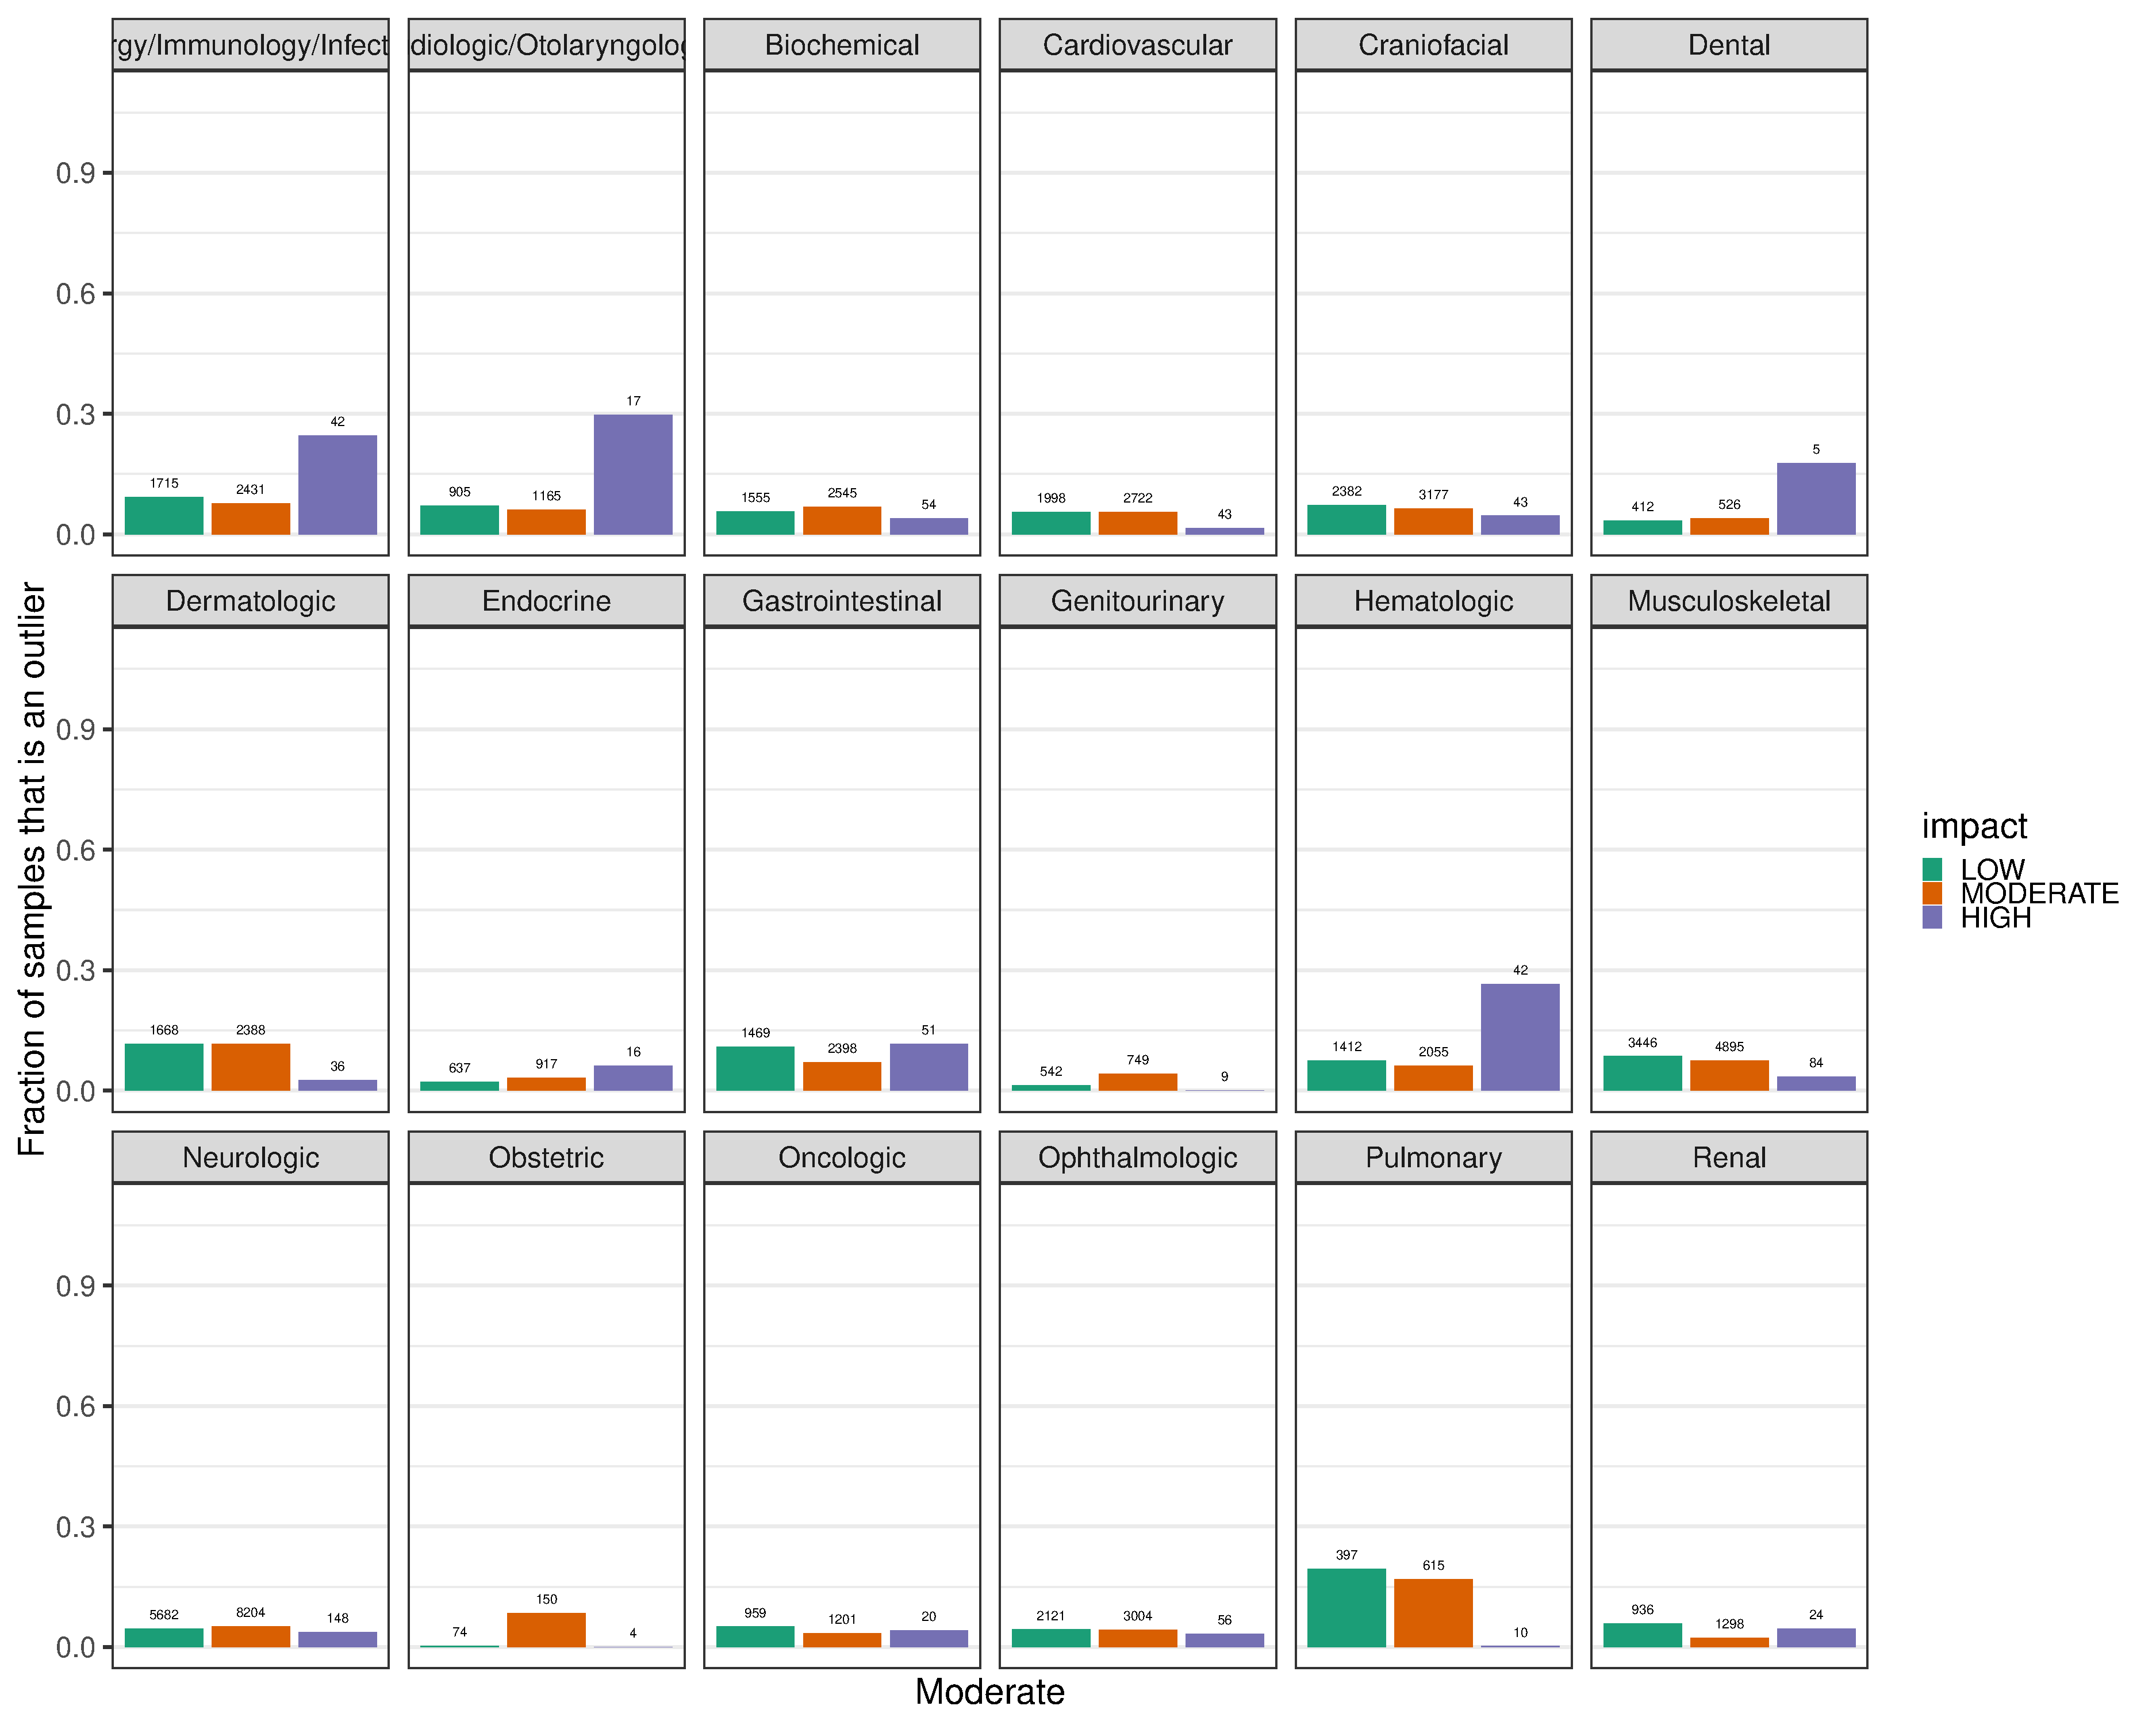
\includegraphics[width=\textwidth]{chapters/chapter3-allele-specific-expression/img/fig3.pdf}
	\caption{\textbf{Comparison of proportion of variants that show allelic imbalance between SnpEff annotated variants for different OMIM disease categories.} Each plot is a different OMIM disease category. The x-axis are SnpEff impact categories. The y-axis is the proportion of variants that belong to that category that show allelic imbalance (binomial FDR p-value $<$ 0.05), e.g. of the 17 high impact SNPs in Audiologic genes, 30\% shows allelic imbalance. The same variant can be counted multiple times if multiple samples carry the same variant. P-values above bars are from fisher exact test, corrected for the total number of tests in this plot using Bonferonni correction. }
	\label{ase_fig3}
\end{figure}


\Needspace{10\baselineskip}
\subsection{Splice donor and acceptor variants are often the cause of allelic imbalance}
We next investigated the functional effect of ASE variants by annotating variants using SnpEff \cite{cingolaniProgramAnnotatingPredicting2012}, a genetic variant annotation and functional effect prediction toolbox. We observed that for some disease categories, predicted high impact variants showed allelic imbalance more often than moderate and low impact variants (\textbf{Supplementary Figure 6}). When examining SnpEff predicted inheritance categories, the high impact variants always showed a higher proportion of allelic imbalance for all inheritance categories that contained high impact variants (Autosomal Dominant (AD), Autosomal Dominant or Autosomal Recessive (AD/AR), Autosomal Recessive (AR), and other, \textbf{Supplementary Figure 7}). The SnpEff categories are partly based on the type of mutation. Within the high impact category, splice donor and acceptor variants showed allelic imbalance more often (64\% and 71\%, respectively) than stop gained, stop loss and start loss variants (41\%, 49\% and 12\%, respectively). When variants were stratified by high impact category, the strongest enrichment (Test of Proportions $p = 4.72 \times 10^{-106}$, \textbf{Supplementary Figure 8}) was observed in the stop gain category. Other categories in which this enrichment is present are start loss ($p = 2.73 \times 10^{-25}$), stop loss ($p = 2.5 \times 10^{-50}$) and splice acceptor sites (p = $5.67 \times 10^{-05}$).


\Needspace{10\baselineskip}
\subsection{Predicted high impact variants under express the minor allele}
The effect of high impact variants might be mitigated if the expression of the haplotype with the disruptive allele is lower than that of the haplotype with the functional allele. To test this, we annotated the geneASE SNPs with SnpEff-predicted impact categories. Here we observed that the minor/major expression ratio of high impact variants showed significantly larger differences than that of moderate (Wilcoxon  test $p = 1.9 \times 10^{-15}$) and low impact variants (Wilcoxon test $p = 6.8 \times 10^{-26}$, \textbf{Figure \ref{ase_fig4}}). We speculate that this is because the high impact variant limits the amount of expression of the haplotype of that allele by having a start loss or stop gain function, possibly leading to nonsense-mediated decay. The major haplotype can compensate for the loss of function of the modified haplotype to keep the overall expression of the gene similar to the baseline expression. One way this can happen is due to a feedback loop from downstream proteins not getting enough correctly binding proteins, initiating the transcription of more RNA of the imbalanced gene. 

\begin{figure}[h!]
	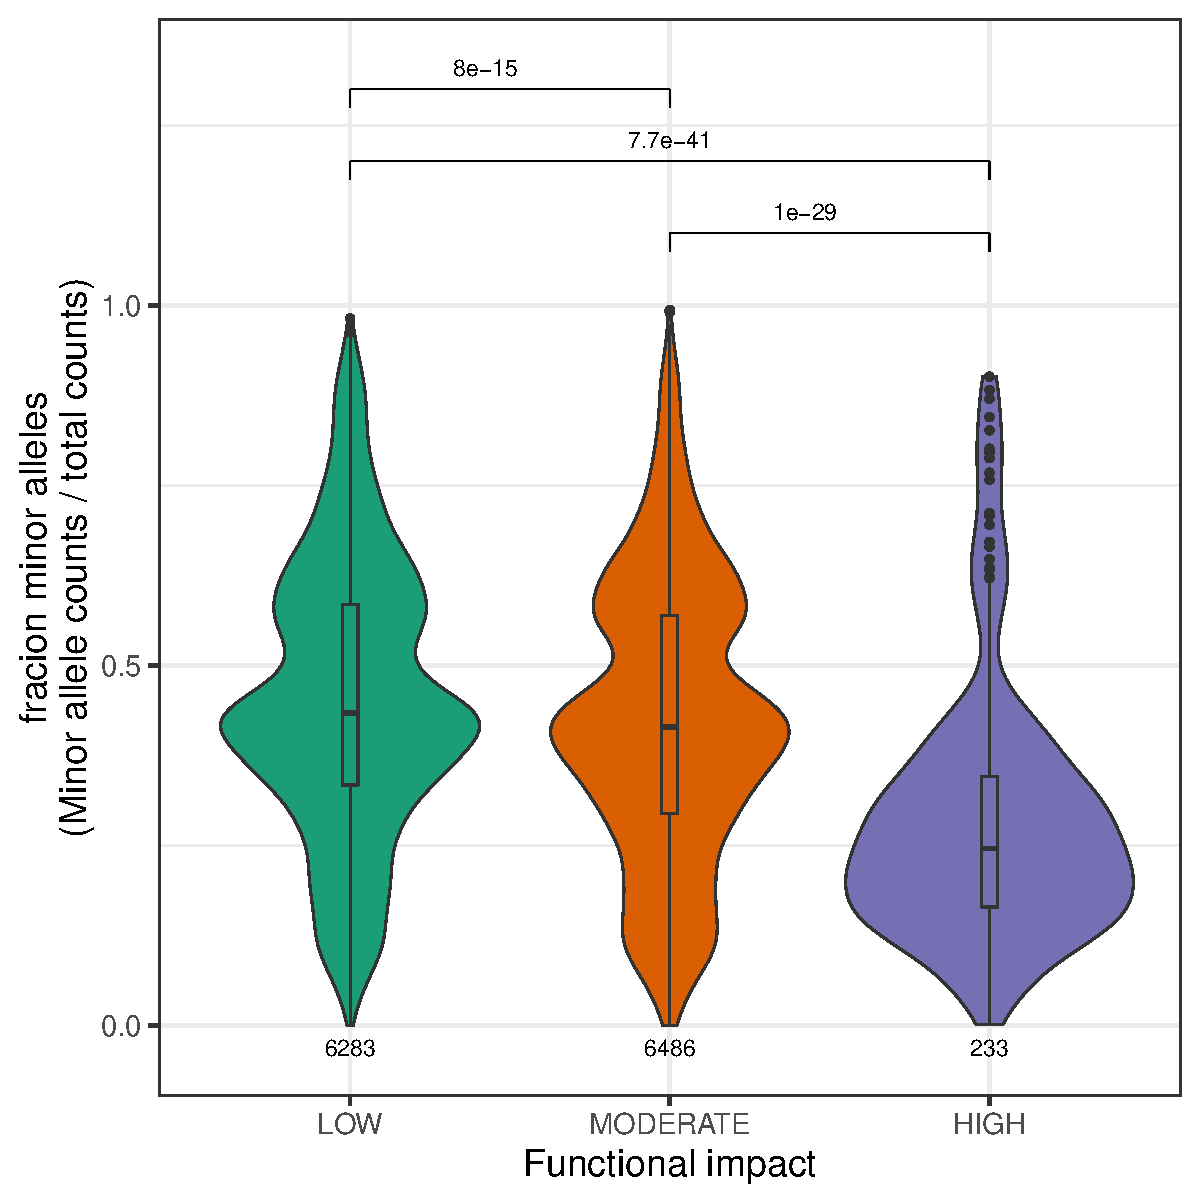
\includegraphics[width=\textwidth]{chapters/chapter3-allele-specific-expression/img/fig4.pdf}
	\caption{\textbf{Fraction of reads overlapping the minor allele compared to major allele for different SnpEFF predicted impact categories.}}
	\label{ase_fig4}
\end{figure}



\Needspace{10\baselineskip}
\subsection{Expression of some genes with autosomal dominant mutations is normal compared to the rest of the population}
Finally, we found that seven individuals carried a total of six high impact (SnpEff-predicted impact = high and CADD phred score $>$ 20) autosomal dominant variants within one of five different genes (\textit{ALOX5}, \textit{COMT}, \textit{PRPF8}, \textit{PSTPIP1} and \textit{SH3BP2}). The allelic depth of five of these seven observations was high ($\geq$ 36 reads on each allele), making it unlikely that they are false positive findings. For two genes, \textit{COMT} and \textit{PRPF8}, the allelic depth was lower (26/6 and 8/40 counts on the reference/alternative allele, respectively) but still deemed sufficient. Of the six variants, one was also observed in array data with a concordant genotype, while the others were not present in the array data because they were too rare to be reliably imputed. 

Since our BIOS participants are mostly healthy, it is unlikely that these autosomal dominant mutations cause severe disease, and thus their penetrance is likely to be low. In order to understand this, we compared the expression levels of all individuals in the BIOS cohort to the expression levels of the seven individuals discussed above and found that their expression was not outside of the norm of the rest of the cohort (\textbf{Figure \ref{ase_fig5}}). Interestingly, in some of these seven individuals, one of the alleles completely rescues the expression levels for that gene. For example, the carrier of a variant in \textit{PRPF8} had average expression for \textit{PRPF8}, but the major allele contributed 80\% of the expression. Interestingly, one sample with a low impact SNP in the same gene shows almost the same gene expression, even though the minor allele contributes 60\% of the total expression for that gene (\textbf{Figure \ref{ase_fig5}}). \textit{PRPF8} is also the only gene out of the 5 that is intolerant to mutations according to its pLI score. For \textit{SH3BP2}, the variant is located at the start of exon 9, which is a non-constitutive exon. 

\begin{figure}[h!]
	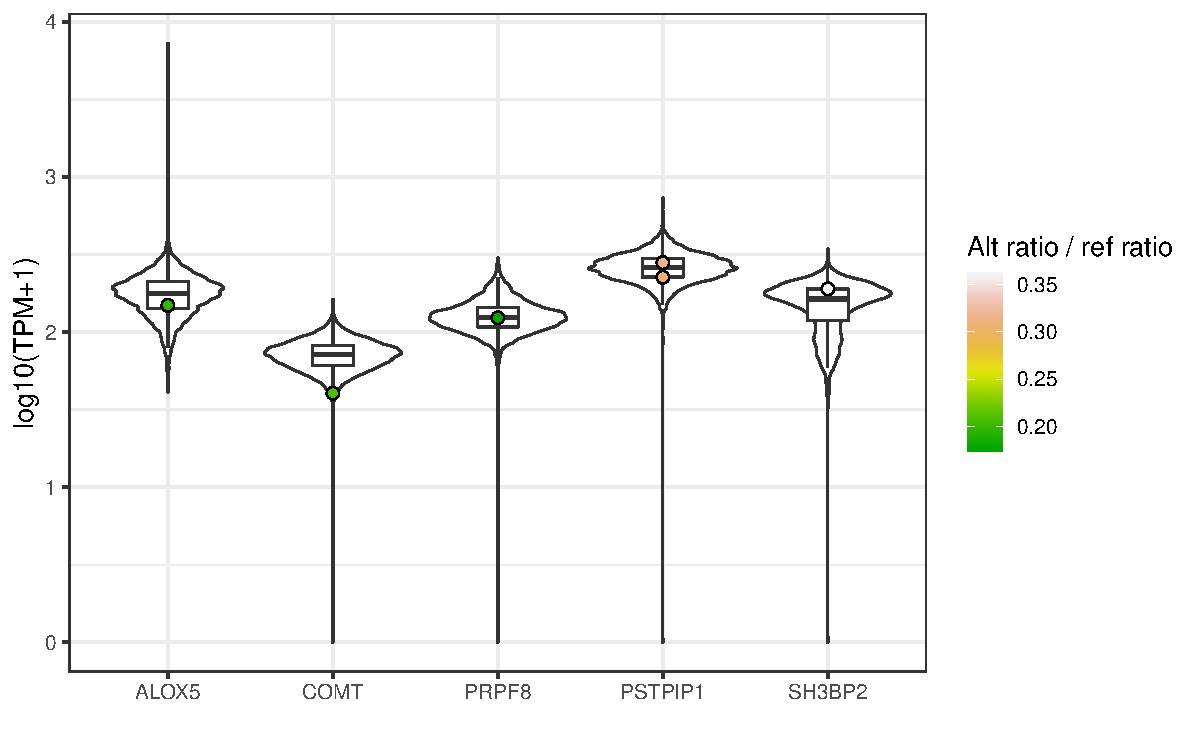
\includegraphics[width=\textwidth]{chapters/chapter3-allele-specific-expression/img/fig5.pdf}
	\caption{\textbf{Expression levels of autosomal dominant variants and variants with different SnpEff impact.} Distribution of expression levels for all samples for six autosomal dominant genes that contain high impact variants (CADD score > 15). The allelic ratio of the sample with the autosomal dominant variant is shown by the dot color.}
	\label{ase_fig5}
\end{figure}

\Needspace{10\baselineskip}
\section{Discussion}

In clinical genetics there are still many cases where a diagnosis cannot be made\cite{diemenRapidTargetedGenomics2017}. For some of these undiagnosed cases, RNA-Sequencing can help make a diagnosis\cite{marco-pucheRNASeqPerspectivesImprove2019}, and outlier ASE has recently been used as diagnostic tool for muscular disease patients\cite{mohammadiGeneticRegulatoryVariation2019}. However, to know what effect a very rare pathogenic variant might have, ASE must be analysed in a large dataset. In this study we explored the effects of rare variants on gene expression in blood in the samples of 3,810 individuals from BIOS, a Dutch population-based consortium. This allowed us to compare the effects of rare variants on gene expression for SNVs with different pathogenicity levels and impact factors for genes in various disease categories.

\Needspace{10\baselineskip}
\subsection{Effects of high impact and pathogenic variants}
We found that pathogenic variants annotated by ClinVar\cite{landrumClinVarImprovingAccess2018} and VKGL\cite{fokkemaDutchGenomeDiagnostic2019} showed allelic imbalance more often than VUS and benign variants. One possible explanation for this is that if the expression of the gene in which the variant is located is altered, this gene could more likely have a phenotypic effect. These variants are only possible to exist if there is compensation for via the other allele. Since the individuals in this study were not known to have a genetic disorder, there should be some compensation for this variant, either through other genes and mechanisms or by recovery of the gene expression through the other allele. This is indeed observed for the autosomal dominant high impact variant in \textit{PRPF8}, where the major allele compensates for the much lower expression of the minor allele. We further observed that predicted high impact variants also showed allelic imbalance more often than moderate and low impact variants, which holds for all disease categories in which there was a gene with high impact variants. Also, between low and moderate impact variants, we often observed much smaller difference between the numbers of variants with allelic imbalance. Genes with high impact variants also showed higher expression on the major allele, although, due to the fact that rare variants (MAF $<$ 0.01) were not masked during read alignment, a somewhat higher expression is expected due to possible reference bias.

\Needspace{10\baselineskip}
\subsection{Limitations of our approach}
There are several limitations to our approach. We examined a healthy population cohort to look at the effects of rare variants, but this obviously limited the number of pathogenic variants. Although we have a large sample size to look at allelic imbalance in blood samples, many effects are not shared between tissues\cite{castelModifiedPenetranceCoding2018}, which may explain why we only find allelic imbalance of pathogenic variants in certain disease categories. This suggests that RNA-Sequencing from blood, while the most readily available tissue in a clinical setting, may only be relevant for a limited number of disease phenotypes. For other diseases, the differences in allelic imbalance were not picked up in blood, most likely because the disease-relevant genes are not sufficiently expressed in this tissue. Finally, even with the relatively large number of individuals, there were only a limited number of known pathogenic variants present in the BIOS cohort. Improvements could be made by increasing the sample size of the study cohort by generating more gene expression profiles or by involving other existing datasets in the meta-analysis. 

\Needspace{10\baselineskip}
\section{Conclusion}
We examined allele specific expression (ASE) within RNA-Seq data for the BIOS cohort in order to see if we could identify differences in ASE effects between known pathogenic or high impact variants and benign or low impact variants. In the future we would like to apply this approach to samples from the clinic to determine if ASE can help in prioritizing disease-relevant variants by identifying VUS with a large allelic imbalance and comparing it to the allelic imbalance found in the same gene for healthy individuals. We have also shown that it is possible to accurately genotype exonic variants and to subsequently phase them using RNA-Seq data, improving on the work of Deelen \textit{et al}.\cite{deelenCallingGenotypesPublic2015}. This can be an added benefit for genome diagnostics. We have also shown that it is possible to identify rare variants that have a strong effect on gene expression data, solely by using RNA-Seq data. Variants known to be pathogenic and located in genes from relevant disease categories show imbalanced allelic expression more often than benign variants in the same gene. VUS show an imbalance in allelic expression at the same or lower rates as benign variants. We hypothesize that variants within the VUS category that show allelic imbalance are more likely to be pathogenic than those that do not. Follow-up studies examining patient data would be interesting to show whether measuring RNA-expression levels in patients would help improve diagnostics.

\Needspace{10\baselineskip}
\section{Material \& Methods}
\Needspace{10\baselineskip}
\subsection{RNA-Seq preparation and data processing in the BIOS cohort}
RNA sequencing methods are described in Zhernakova \textit{et al}.\cite{zhernakovaIdentificationContextdependentExpression2017} The RNA-Seq data was prepared in two different ways. For expression level quantification and mapping of reads for ASE analysis, we used the BAM files from (Zhernakova \textit{et al}. 2017). In short, the generated fastq files were first checked on read quality using FastQC\cite{andrewssimonandothersFastQCQualityControl2010} software. Second, adaptor sequences were trimmed using CutAdapt (v1.1)\cite{martinCutadaptRemovesAdapter2011} with default settings. Third, Sickle (v1.200)\cite{joshinaandfassjnandothersSickleSlidingwindowAdaptive2011} was used to remove low quality read ends. All reads were aligned using STAR v2.3.0e\cite{dobinSTARUltrafastUniversal2013}. To avoid reference mapping bias, all SNPs present in the Genome of the Netherlands (GoNL)\cite{francioliWholegenomeSequenceVariation2014} dataset with a MAF $\geq$ 0.01 were masked during alignment. Read pairs mapping to at most five positions and having at most eight mismatches were retained for downstream analyses. Subsequent gene quantification was done on Ensembl\cite{cunninghamEnsembl20192019} build v71 (which corresponds to GENCODE\cite{frankishGENCODEReferenceAnnotation2019} v16).
For genotype calling, the alignment of RNA-Seq data was done using the UCSC genome build 37, as defined in the 1000 Genomes project (bundle 2.8, downloaded: ftp://gsapubftp-anonymous@ftp.broadinstitute.org/bundle/), using Hisat\cite{kimHISATFastSpliced2015} version 0.1.6-beta and default settings. Unlike the mapping for the ASE analysis, the genome was not masked. Subsequently, the SAM alignment files generated were filtered using SAMtools\cite{liSequenceAlignmentMap2009} (v1.2) to only contain uniquely mapping reads and afterwards converted to BAM format, sorted on genomic position and indexed using Picard tools\cite{broadinstitutePicardTools2016} version 1.102.

\Needspace{10\baselineskip}
\subsection{Data processing and genotype calling}
Aligned reads were processed using several command line tools from the Picard tools v1.102 set. Aligned reads were assigned read groups using Picard tools’ AddOrReplaceReadGroups. All BAM files that passed QC were merged to a single BAM file per sample according to the QC outcome of the concordance checks from Picard’s MergeSamFiles. 
Picard tools MarkDuplicates marked all duplicate reads, which indicate PCR artefacts, and these duplicates were not used in subsequent analysis. 
Further read adjustment was done using GATK version 3.4.0. To prevent false discovery of incorrectly spliced reads, reads including N cigar elements were split using GATK SplitNCigarReads with parameter ReassignOneMappingQuality set to 255 and 60, assuring hard clipping of overhanging reads and assigning the correct quality value of 60 to high quality mapping sites. For realignment around indels, GATK IndelRealigner was run with the 1000 genomes phase 1\cite{n1000GenomesProject2008} and Mills \textit{et al}.\cite{millsInitialMapInsertion2006} data set as the gold standard data set. 
A phred-scaled quality score was associated with every base. After adjusting reads as described, GATK BaseRecalibrator was used to recalibrate the base quality scores using information from the base cycle, base context and original base quality score, taking into account known variant sites from dbSNP, the 1000 genomes project\cite{n1000GenomesProject2008} and the Mills \textit{et al}.\cite{millsInitialMapInsertion2006} gold standard set. 
Initial haplotypes were constructed using GATK HaplotypeCaller emitting sites in gVCF mode. The gVCF mode generates VCF files in which information of genomic regions is also captured. This information is used downstream to call variants on the complete cohort of samples.
To speed up genotype calling on cohort level, we used a custom-made Python script (\url{https://github.com/molgenis/ngs-utils/blob/master/generate\_merge\_vcf\_jobs.py}) to generate jobs that merge 200 gVCF files using GATK CombineGVCFs into a single vcf file to be used as input in the next analysis step.
The final call set was generated using GATK GenotypeGVCFs. We used all merged gVCFs containing 200 samples each as input and set a call confidence threshold of 10.0 and an emit confidence of 20.0. This approach ensured that all individual-level SNP information required for downstream analysis were present.

\Needspace{10\baselineskip}
\subsection{Concordance between RNA-Seq genotypes and WGS genotypes}
Phased WGS genotype VCF files were obtained from the GoNL project\cite{francioliWholegenomeSequenceVariation2014}. The 249 GoNL samples that were included for the ASE project were selected from the VCF file, and the allele frequency was recalculated. The same 249 samples were selected from the RNA-Seq-based genotype VCF files, and allele frequency was re-calculated. Plots were made using \url{https://github.com/npklein/BIOS\_ASE/blob/master/concordance\_GoNL\_DNA\_vs\_RNA.R}. 

\Needspace{10\baselineskip}
\subsection{Alignment quality control}
FastQC (\url{http://www.bioinformatics.babraham.ac.uk/projects/fastqc/}) was used to check quality metrics, and we removed individuals with $<$ 70\% of reads mapping to exons (exon mapped/genome). To assess the alignment quality per sample the Picard Tools CollectMultipleMetrics, CollectRNA-SeqMetrics and SAMtools flagstat were executed on all sample-level BAM files.

\Needspace{10\baselineskip}
\subsection{Filtering of the genotype call set}
We included only unrelated individuals and removed population outliers by filtering out samples $>$3 standard deviations from the average heterogeneity score. Low quality variants and sites where many samples do not have a genotype call can badly bias genotype calling and phasing. We therefore filtered all variants in the call set on two criteria: call rate of at least 50\% and per sample genotype quality of at least 20. Filtering was performed using a custom Perl script (\url{https://github.com/freerkvandijk/miscellaneous/blob/master/filterRNA-SeqCallsV2.pl}). Variants for which all genotypes were set to missing after applying the filter were completely removed from the call set. We filtered our call set to keep only biallelic sites using GATK SelectVariants with the parameters -selectType SNP and -restrictAllelesTo BIALLELIC.

\Needspace{10\baselineskip}
\subsection{eQTL and ASE replication}
To replicate the ASE effects in eQTLs and ASE, the major and minor counts per variant were summed over all samples for SNPs where at least 30 samples are heterozygous. The ratio of the ASE effect was calculated as: (minor allele counts) / (major allele counts). The P-value was calculated with a binomial test, with 0.5 as expected value for the minor over total counts, and adjusted for multiple testing with Benjamini-Hochberg method\cite{benjaminiControllingFalseDiscovery1995}. The ASE ratio is centred on 0 so that for values $<$ 0 the minor allele has lower expression than the major allele and for values $>$ 0 the minor allele has higher expression than the major allele.
To replicate the effect in eQTLs, cis-eQTLs were calculated in the BIOS dataset for only the SNP–gene pairs for which we obtained an ASE score for SNPs with MAF $>$ 0.01, call rate $>$ 0.95 and Hardy-Weinberg $>$ 0.0001. If the assessed allele of the eQTLs was not the same as the minor allele of the ASE SNP, the z-score was flipped. FDR for the eQTLs were calculated using a permutation strategy, as described previously in Westra \textit{et al}.\cite{westraSystematicIdentificationTrans2013} SNPs where both the ASE effect and the eQTL effect FDR were $<$ 0.05 were used in the comparison.
To replicate the effect in GTEx, GTEx ASE counts were downloaded from the GTEx portal (\url{https://www.gtexportal.org/home/datasets}) and harmonized to the BIOS minor allele. P-values for the GTEx effects were calculated using a binomial test and corrected for multiple testing using the Benjamini-Hochberg method. For both BIOS and GTEx, SNPs were only included if at least 30 samples were heterozygous.
To replicate ASE effects in LCL cells, an LCL ASE dataset\cite{deelenCallingGenotypesPublic2015} was downloaded from \url{https://molgenis56.target.rug.nl/menu/main/dataexplorer?entity=ASE}. LCL SNPs that overlapped with BIOS ASE SNPs and had an FDR corrected p-value $<$ 0.05 were used for comparison.

\Needspace{10\baselineskip}
\subsection{Phasing of low coverage genotype call set}
For parallelization, the genome was chunked by selecting all genes expressed in blood (expressed gene list can be downloaded from \url{https://github.com/molgenis/molgenis-pipelines/blob/master/compute5/BIOS\_phasing/scripts/expressedGenesBlood20170213.txt}), merging the overlapping chunks, and subsequently extending the chunk range to the neighbouring chunks. All subsequent phasing steps were done per chunk. Missing genotypes were filled in with Beagle\cite{browningGenotypeImputationMillions2016} v.4.1 version 27Jul16.86a (beagleVCF). A separate VCF was generated with the phred-scaled likelihoods converted to genotype likelihoods using a custom script (\url{https://github.com/molgenis/ngs-utils/blob/master/PL\_to\_GL\_reorder.py}, adjusted from \url{https://github.com/team149/tc9/blob/master/conversion/PL2GL.py}). beagleVCF and likelihoodVCF were converted to Shapeit2 format using prepareGenFromBeagle \url{(https://mathgen.stats.ox.ac.uk/genetics\_software/shapeit/files/prepareGenFromBeagle4.tgz}). Subsequently, the converted VCF files, together with the original input VCF files, were converted to Shapeit2 format using prepareGenFromBeagle (\url{https://mathgen.stats.ox.ac.uk/genetics\_software/shapeit/files/prepareGenFromBeagle4.tgz}).
	
\Needspace{10\baselineskip}
\subsection{Read-backed phasing and allelic count generation}
Read-backed phasing can be used to improve phasing of variants, especially rare variants, that influence splicing. We used phASER\cite{castelRareVariantPhasing2016} (version 1.0.0, git version cd7daba) to perform read-backed phasing for all samples in combination with the RNA-Seq BAM files. PhASER ran with the following options: -paired-end, -gw\_phase\_method, -gw\_phase\_vcf, -baseq 10 and -mapq 255, allowing only uniquely mapped reads to be used for counting of alleles. In addition to these options, we also enabled the -unphased\_vars, which is required to run phASER Gene AE afterwards.
phASER provides haplotypic counts for blocks of overlapping RNA reads. With GeneAE, the haplotypes that overlap a gene are summed to give a genetic feature count. For each sample and gene, the results are aggregated into a matrix with an allelic ratio for each gene and each sample. 

\Needspace{10\baselineskip}
\subsection{Job generation, execution and monitoring}
The genotype calling from the RNA-Seq data described above was conducted by implementing all commands in bash protocols. Each protocol contains the commands, settings and variables, which are filled in during generation time by the MOLGENIS Compute framework\cite{byelasMOLGENISBasedComputational2011}. This framework enables the generation of bash scripts for use on several cluster environments by combining information from a workflow file, parameter file and sample sheet containing detailed information about samples. All pipelines can be found here: \url{https://github.com/molgenis/molgenis-pipelines/}. We used Public\_RNA-Seq\_QC, Public\_RNA-Seq\_genotypeCalling and BIOS\_phasing with commit version d44386698818cf422715db56a9b8e3da1e06d586 for all analyses. 

\Needspace{10\baselineskip}
\subsection{Annotating variants with functional information}
Variants were annotated using SnpEff\cite{cingolaniProgramAnnotatingPredicting2012} (v4.3) with the parameters -lof, -canon, -ud 0. Subsequently, the SnpEff closest was used to annotate variants to their closest genomic region. Additional allele frequency information from ExAC and GoNL were added using a custom script (\url{https://github.com/npklein/BIOS\_ASE/blob/master/annotateVariantTablesWithExACandGoNLAlleleFrequency.pl}).

\Needspace{10\baselineskip}
\subsection{Processing allelic counts}
A walkthrough of all steps can be found at \url{https://github.com/npklein/BIOS\_ASE}. GeneAE counts from phASER\cite{castelRareVariantPhasing2016} were converted to a matrix with haplotype A and matrix with haplotype B counts (See \url{https://github.com/npklein/BIO\_ASE/blob/master/createCountTables.pl}). For each gene of each sample, a binomial p-value was calculated using a two-sided binomial test with expected proportion = 0.5 and confidence level = 0.95. P-values were corrected for multiple testing using Benjamini-Hochberg method\cite{benjaminiControllingFalseDiscovery1995} (\url{https://github.com/npklein/BIOS\_ASE/blob/master/ASE\_binomial\_test/binom\_test.R}). For each of our samples, the number of genes with a significant ASE effect were counted, and five samples with $>$ 500 genes with an ASE effect were filtered out based on visual identification of outlier samples (\url{https://github.com/npklein/BIOS\_ASE/blob/master/createGenesAndOutliersTable.pl} and \url{https://github.com/npklein/BIOS\_ASE/blob/master/removeOutliersAndCODAM.R}). In addition, one sample was removed because it had a very low genotype concordance with the WGS data. For all 3,810 samples, the haplotype A and B counts were harmonized against the reference genome after filtering (\url{https://github.com/npklein/BIOS\_ASE/blob/master/minor\_allele\_ratio/createTable.pl}). SNPs were annotated with ClinVar pathogenicity information (v2018-Nov-16), CADD scores\cite{kircherGeneralFrameworkEstimating2014} and SnpEff information (\url{https://github.com/npklein/BIOS\_ASE/blob/master/minor\_allele\_ratio/annotateCountsWithCADD.pl}), and genes in which SNPs are located were annotated with OMIM disease information (\url{https://github.com/npklein/BIOS\_ASE/blob/master/figure\_2\_and\_3/OMIM\_enrichment.py}). For the different impact categories of ClinVar, allele ratios were calculated per impact category (\url{https://github.com/npklein/BIOS\_ASE/blob/master/minor\_allele\_ratio/plot\_minor\_vs\_major\_20190129.R}). Per disease category, we calculated the enrichment of genes that show an ASE effect (\url{https://github.com/npklein/BIOS\_ASE/blob/master/figure\_2\_and\_3/enrichment\_disease\_genes\_in\_outliers\_per\_category.py}). 

\section*{Data availability}
The RNA-Seq, DNA methylation, sex, age and cell count data (but not genetic and more extended phenotype data) can be requested and downloaded from the European Genome-phenome Archive (EGA) using accession number EGAS00001001077. All gene and sample ASE data is available in an online browser that can be accessed via \url{https://molgenis15.gcc.rug.nl/}. All scripts to plot the main and supplemental figures are available in our github repository: \url{https://github.com/npklein/BIOS\_ASE}.

\section*{Acknowledgements}
We thank K. Mc Intyre for editing the final text. F.v D. is supported by the Netherlands CardioVascular Research Initiative: "the Dutch Heart Foundation, Dutch Federation of University Medical Centres, the Netherlands Organisation for Health Research and Development and the Royal Netherlands Academy of Sciences" (CVON2011-19). L.F. is supported by grants from the Dutch Research Council (ZonMW-VIDI 917.164.455 to M.S. and ZonMW-VIDI 917.14.374 to L.F.), by an ERC Starting Grant, grant agreement 637640 (ImmRisk) and by an Oncode Senior Investigator Grant. The Biobank-Based Integrative Omics Studies (BIOS) Consortium is funded by BBMRI-NL, a research infrastructure financed by the Dutch government (NWO 184.021.007). We thank the UMCG Genomics Coordination Center, the UG Center for Information Technology and their sponsors BBMRI-NL \& TarGet for storage and compute infrastructure.


\newpage
\bibliographystyle{naturemag}
{\footnotesize
	\bibliography{chapters/chapter3-allele-specific-expression/chapter3-ase}}
\leftwatermark{}
\rightwatermark{}
\chapterfont{\huge\color{DarkBlue}}  % sets colour of chapter
\sectionfont{\color{DarkBlue}}  % sets colour of sections
\subsectionfont{\color{DarkBlue}}  % sets colour of subsections

\renewcommand\pcolor{DarkBlue}
\renewcommand{\headrule}{\hbox to\headwidth{%
		\color{DarkBlue}\leaders\hrule height \headrulewidth\hfill}} % color of title
\fancyfoot[LE,RO]{\thepage}

{ \Large \leftwatermark{
		\put(-67,-66.5){ 1 }
		\put(-67,-91.5){ 2 }
		\put(-67,-116.5){ 3 }
		\put(-76.5,-151){
\includegraphics[scale=0.8]{img/thumbindex/thumbindex_DarkBlue.eps}}  
		\put(-67,-141.5){{\color{white} 4 }}
		\put(-67,-166.5){ 5 }
		\put(-67,-191.5){ 6 }
	} \rightwatermark{
		\put(350.5,-66.5){ 1 }
		\put(350.5,-91.5){ 2 }
		\put(350.5,-116.5){ 3 }
		\put(350.5,-151){
\includegraphics[scale=0.8]{img/thumbindex/thumbindex_DarkBlue.eps}}  
		\put(350.5,-141.5){ {\color{white} 4 } }
		\put(350.5,-166.5){ 5 }
		\put(350.5,-191.5){ 6 }
}}

\cleardoublepage
\makeatletter
\let\savedchap\@makechapterhead
\def\@makechapterhead{\vspace*{-3cm}\savedchap}
\chapter[Deconvolution of bulk blood eQTL effects into immune cell sub-populations]{Deconvolution of bulk blood eQTL effects into immune cell sub-populations}

\label{chap:chapter4-deconvolution}
\chaptermark{}
\let\@makechapterhead\savedchap
\makeatletter


\hfill \underline{BMC Bioinformatics} 2020 June 12; Volume 21: p1-23.

\hfill DOI: \href{https://doi.org/10.1186/s12859-020-03576-5}{s12859-020-03576-5}
\\
\\
Raul Aguirre-Gamboa1\textsuperscript{*}, Niek de Klein\textsuperscript{*}, Jennifer di Tommaso\textsuperscript{*}, Annique Claringbould,Monique van der Wijst, Dylan de Vries, Harm Brugge, Roy Oelen, Urmo Võsa, Maria Zorro, Xiaojin Chu, Olivier B. Bakker, Zuzanna Borek, Isis Ricaño-Ponce, Patrick Deelen, Cheng-Jiang Xu, Morris Swertz, Iris Jonkers, Sebo Withoff, Irma Joosten, Serena Sanna, Vinod Kumar, Hans J.P.M. Koenen, Leo A.B. Joosten, Mihai G. Netea, Cisca Wijmenga, BIOS Consortium, Lude Franke\textsuperscript{\#}, Yang Li\textsuperscript{\#}
\\
\\
* These authors contributed equally to this work. \\
\# These authors jointly directed this work

\newpage

\section*{Abstract}

Expression quantitative trait loci (eQTL) studies are used to interpret the function of disease-associated genetic risk factors. To date, most eQTL analyses have been conducted in bulk tissues, such as whole blood and tissue biopsies, which are likely to mask the cell type context of the eQTL regulatory effects. Although this context can be investigated by generating transcriptional profiles from purified cell sub-populations, the current methods are labor-intensive and expensive. Here we introduce a new method, \textit{Decon2}, a framework for estimating cell proportions using expression profiles from bulk blood samples (Decon-cell) followed by deconvolution of cell type eQTLs (Decon-eQTL). The estimated cell proportions from Decon-cell agree with experimental measurements across cohorts ($R \geq 0.77$). Using Decon-cell we can predict the proportions of 34 circulating cell types for 3,194 samples from a population-based cohort. Next we identified 16,362 whole blood eQTLs and deconvoluted cell type interaction (CTi) eQTLs using the predicted cell proportions from Decon-cell. CTi eQTLs show excellent allelic directional concordance with those of eQTL($\geq$ 96\%-100\%) and chromatin mark QTL ($\geq$ 87\%-92\%) studies that used either purified cell sub-populations or single-cell RNA-seq, outperforming the conventional interaction effect. Decon2 provides a method to detect cell type interaction effects from bulk blood eQTLs, which is useful in pinpointing the most relevant cell type for a certain complex disease. Decon2 is available as an R package and Java application (\url{https://github.com/molgenis/systemsgenetics/tree/master/Decon2}), and as a web tool (www.molgenis.org/deconvolution).


\Needspace{10\baselineskip}
\section{Introduction}

For many of the genetic risk factors that have been associated to immune diseases by genome-wide association studies (GWAS), the molecular mechanism leading to disease remains unknown\cite{hindorffPotentialEtiologicFunctional2009}. Most of these genetic risk variants are located in the non-coding regions of the genome, implying that they play a role in gene regulation\cite{ionita-lazaSpectralApproachIntegrating2016,javierreLineageSpecificGenomeArchitecture2016}. Expression quantitative trait locus (eQTL) analysis provides a way to characterize the regulatory effect of these risk factors in humans, and many eQTL studies have now been carried out using bulk tissues, for example, whole blood\cite{westraSystematicIdentificationTrans2013,joehanesIntegratedGenomewideAnalysis2017}. However, bulk tissues comprise many different cell types, and gene regulation is known to vary across cell types\cite{rajPolarizationEffectsAutoimmune2014,petersInsightGenotypePhenotypeAssociations2016,naranbhaiGenomicModulatorsGene2015}. In recent years, efforts to describe eQTL effects in purified cell sub-populations have been carried out in specific cell types\cite{chenGeneticDriversEpigenetic2016}. Unfortunately, the length and cost of the study protocols have limited these studies to small sample sizes and only a few cell types. Current developments on single cell (sc) RNASeq technologies have given rise to sc-eQTLs, such approach although promising is still bound to a limited number of individuals limiting the number of detectable cell type (CT) eQTLs. Nevertheless, being able to pinpoint the particular CT in which a risk factor exerts an eQTL effect could help us to understand its role in disease.

Statistical approaches to detect CT effects using tissue expression profiles have mainly been developed to evaluate gene by environment interaction (GxE) terms, for example, being able to detect CT eQTLs for myeloid and lymphoid lineages using only whole blood gene expression and by evaluating the interaction between genotype and cell proportions for neutrophils and lymphocytes in whole blood\cite{westraCellSpecificEQTL2015}. A second study linked eQTL genes to proxy genes through correlation; these proxy genes were then associated with intrinsic or extrinsic factors, such as cell proportions or inflammation markers\cite{zhernakovaIdentificationContextdependentExpression2017}. However, these efforts focused on exploiting only one GxE term, or on indirectly linking the CT proportions to given eQTL instead of directly ascertaining the interaction between all the main cell proportions comprising the bulk tissue and genotype. Unfortunately, quantifying cell proportions, in particular for rare sub-populations (total abundance of $\leq 3\%$ in circulating white blood cells), is expensive and time-consuming. Hence, quantifying immune cell proportions in large functional genomics cohorts is not common practice.

Here we present and validate \textbf{Decon2}, a computational and statistical framework that can: (1) predict the proportions of known circulating immune cell sub-populations (\textbf{Decon-cell}), and (2) use these predicted proportions along with whole blood gene expression and genotype information to assign bulk eQTL effects into CT eQTLs (\textbf{Decon-eQTL}). Our two-step framework provides an improvement over previously published methods. Unlike earlier methods\cite{aranXCellDigitallyPortraying2017}, Decon-cell does not rely on any prior information of transcriptome profiles from purified cell sub-populations, as it only requires the quantification of the cell proportions comprising the bulk tissue, in this case whole blood. Decon-cell identifies  signature genes that correlate with cell proportions in a bulk tissue. Secondly, Decon-eQTL is the first approach in which all major cell proportions (the major cell types for which the sum of proportions per sample to approximately 100\%) of bulk blood tissue are incorporated into an eQTL model simultaneously. Decon-eQTL can then be used to systematically test for any significant interaction between each CT and genotype, while at the same time controlling the effect on expression of the other cell types.

We generated the Decon-cell predictive models using data from the  500FG cohort\cite{neteaUnderstandingHumanImmune2016}, where quantification of immune cell types was carried out using FACS\cite{aguirre-gamboaDifferentialEffectsEnvironmental2016} and RNA-Seq based bulk whole blood transcriptome profiles were available for 89 samples\cite{bakkerIntegrationMultiomicsData2018}. By using a cross-validation approach we were able to accurately predict 34 out of 73 cell subtypes using solely whole blood gene expression. For validation, we applied Decon-cell to three independent cohorts (Lifelines Deep\cite{tigchelaarCohortProfileLifeLines2015}, n = 627, Leiden Longevity cohort\cite{deelenGenomewideAssociationMetaanalysis2014}, n = 660 and the Rotterdam Study\cite{hofmanRotterdamStudy20162015}, n = 773) with both blood RNA-seq and measured cell proportion data available (neutrophils, lymphocytes and CD14+ monocytes and granulocytes). Additionally, we benchmarked Decon-cell prediction performance against two other existing methods that quantify immune cell composition using gene expression profiles from whole blood on these three independent cohorts. After showing that we can accurately predict circulating immune cell proportions, we applied Decon-cell to estimate cell proportions in 3,194 individuals from the BIOS cohort\cite{tigchelaarCohortProfileLifeLines2015,greevenbroekCrosssectionalAssociationInsulin2011,schoenmakerEvidenceGeneticEnrichment2006,willemsenNetherlandsTwinRegister2010}, in which both whole blood RNA-seq and genotypes were available. The BIOS cohort is a valuable resource for functional genomics studies where extensive characterization of the genetic component on gene expression\cite{zhernakovaIdentificationContextdependentExpression2017} and epigenetics\cite{bonderDiseaseVariantsAlter2017} have been performed. We integrated whole blood expression, genotype information and predicted cell proportion with Decon-eQTL, to deconvolute 16,362 significant whole blood cis-eQTLs top effects into CT interacting eQTLs (CTi eQTLs). These deconvoluted CTi eQTL results were comprehensively validated using transcriptome profiles from purified cell sub-populations\cite{adamsBLUEPRINTDecodeEpigenetic2012}, eQTLs and chromatin mark QTLs from purified cell types\cite{chenGeneticDriversEpigenetic2016}, and eQTLs from single-cell experiments\cite{wijstSinglecellRNASequencing2018}. We also systematically compared the performance of Decon-eQTL against previously published methods\cite{westraCellSpecificEQTL2015,zhernakovaIdentificationContextdependentExpression2017} that detect cell type eQTL effects using whole blood expression profiles. 

\begin{figure}[H]
	\includegraphics[width=\textwidth]{chapters/chapter4-deconvolution/img/fig1.png}
	\caption{\textbf{Workflow of application of Decon2 to predict cell counts followed by deconvolution of whole blood eQTLs.} Using whole blood expression and FACS data of 500FG samples, Decon-cell predicts cell proportions with selected marker genes of circulating immune cell subpopulations. Validations of Decon-cell were carried out on three independent cohorts for which measurements of neutrophils/granulocytes, lymphocytes and monocytes CD14+ were available along with expression profiles of whole blood. Benchmarking of Decon-cell was performed against CIBERSORT\cite{newmanRobustEnumerationCell2015} and xCell\cite{aranXCellDigitallyPortraying2017}. Decon-cell was applied to an independent cohort (BIOS) to predict cell counts using whole blood RNA-seq. Decon-eQTL subsequently integrates genotype and tissue expression data together with predicted cell proportions for samples in BIOS to detect cell type eQTLs. We validated Decon-eQTL using multiple independent sources, including expression profiles of purified cell subpopulations, eQTLs and chromatin mark QTLs (cmQTLs) from purified neutrophils, monocytes CD14+ and CD4+ T cells\cite{chenGeneticDriversEpigenetic2016}, and single-cell eQTL results\cite{wijstSinglecellRNASequencing2018}. Benchmarking of Decon-eQTL was carried out for comparison with a previously reported methods that detected cell type–eQTL effects using whole blood expression data, i.e. the Westra \textit{et al.}\cite{westraCellSpecificEQTL2015}}
	\label{decon_fig1}
\end{figure}

\Needspace{10\baselineskip}
\section{Results}
\Needspace{10\baselineskip}
\subsection{Decon-cell accurately predicts the proportions of known immune cell types}
In order to assign the cell types from which an overall eQTL effect from a bulk tissue sample (e.g. whole blood) comes from, we need three types of information: genotype data, tissue expression data, and cell type proportions (\textbf{Figure \ref{decon_fig1}}). Here, we propose a computational method for predicting the cell proportions of known immune cell types using gene signatures in whole blood expression data by employing a machine-learning approach. Decon-cell employs the regularized regression method elastic net25 to define sets of signature genes for each cell type. In other words, these signatures were selected as having the best prediction power for individual cell proportions. 

There are 89 samples in the 500FG cohort with both whole blood RNA-seq and quantification of 73 immune cell sub-populations by FACS available. This data was used to build the prediction models for estimating cell sub-populations by Decon-cell. First we determined which of the 73 cell sub-populations could be reliably predicted by Decon-cell. A within-cohort cross-validation strategy was employed by randomly dividing 89 samples (\textbf{Figure \ref{decon_fig1}}) into training and test sets (70\% and 30\% of the samples, respectively). After generating a model using each training set, we applied the prediction models of each cell type to the samples in the test sets. We compared the predicted and measured cell proportion for each cell type using Spearman correlation coefficients to evaluate the  prediction performance. We repeated this process 100 times and then used the mean of the correlation coefficient in all 100 iterations to evaluate the prediction performance. We were able to predict 34 out of 73 cell sub-populations using whole blood gene expression data at a threshold of mean $R \geq 0.5$ across all 100 iterations (\textbf{Figure \ref{decon_fig2}A}, \textbf{Supplementary Figure 1}, \textbf{Supplementary Table 1}). The number of signature genes selected in the models for predicting cell proportions varied across the cell types, ranging from 2 to 217 signature genes (\textbf{Supplementary Figure 2A}, \textbf{Supplementary Table 1}); and it was independent of the average abundance of these cell types in whole blood ($R = 0.02$, Spearman correlation coefficient, \textbf{Supplementary Figure2A}). In particular, cell types that are abundant in whole blood (granulocytes-neutrophils, CD4+ T-cells, CD14+ monocytes) were predicted with high confidence (correlation between predicted and measured values, $R \geq 0.73$). Remarkably, we were also able to predict a number of less abundant cell sub-populations, including NK cells, CD8+ T-cells, non-NK T-cells (CD3- CD56-), CD4+ central memory, CD4+ effector memory T-cells, and regulatory T-cells (\textbf{Supplementary Figure 2A}) as determined by FACS. Cell types with a low prediction performance ($R < 0.5$) are those that have few signature genes whose expression levels correlate sufficiently (i.e. absolute $R < 0.3$) with the actual cell proportions in whole blood (\textbf{Supplementary Figure 2B-C}). For each of the 34 predictable cell types, we used Decon-cell to build models for predicting their cell counts using all 89 samples from the 500FG cohort. These models were applied to 3,194 samples in an independent cohort (BIOS cohort), to predict cell proportions of circulating immune cell types for the subsequent deconvolution of eQTL effect. 

In addition to within-cohort validation, we tested our cell proportion models using three independent cohorts (LLDeep, $n = 627$, LLS, $n = 660$, $RS, n = 773$), for which cell type abundances were quantified using a Coulter counter for neutrophils (granulocytes for RS), lymphocytes, and CD14+ monocytes (\textbf{Figure \ref{decon_fig2}B}, \textbf{Supplementary Figure 3A-B}). In LLDeep we were able to accurately predict these three cell types with Spearman correlation coefficients of $R = 0.73$, $R = 0.89$, and $R = 0.73$, respectively.  For LLS and RS the prediction performance was also accurate for neutrophils and lymphocytes, but less so for monocytes ($R= 0.76$ for neutrophils, $R = 0.84$ for lymphocyte and $R = 0.50$ for CD14+ monocytes and proportions in LLS, $R = 0.74$ for granulocytes, $R = 0.83$ for lymphocytes and $R = 0.28$ for CD14+ monocytes and in RS). 

Next, in order to benchmark Decon-cell we have compared its prediction performance against two other existing tools that quantify the abundance of known immune cell types using bulk whole blood expression profiles: CIBERSORT\cite{newmanRobustEnumerationCell2015} and xCell\cite{aranXCellDigitallyPortraying2017}. We obtained the predicted proportions by CIBERSORT and enrichment scores of circulating immune cells by xCell for the samples in three different cohorts: LLDeep, LLS and RS (\textbf{Supplementary Figure 4A-B}). For each cell type, Decon-cell outperforms CIBERSORT and xCell (\textbf{Supplementary Figure 3B}). The scatterplots of predicted vs measured values  (\textbf{Supplementary Figure 3A}, and \textbf{Supplementary Figure 4 A-B}) further demonstrate that the better performance of Decon-cell is not due to cell proportion outliers.

Finally, we evaluated whether the signature genes showed CT expression in their relevant purified cell types, using the BLUEPRINT\cite{adamsBLUEPRINTDecodeEpigenetic2012} RNA-seq data from the purified cell sub-populations. We focused on cell types with more than three samples measured, which include neutrophils, CD14+ monocytes, CD4+ T-cells and B-cells. The signature genes showed overall higher expression in their relevant cell sub-populations compared to other cell sub-populations. Interestingly, the signature genes were also able to cluster the samples of the relevant CT using unsupervised hierarchical clustering (\textbf{Supplementary Figure 5A-D}). Together, our results demonstrated that the gene signatures identified by Decon-cell were predictive for the proportions of circulating immune cell sub-populations using only whole blood gene expression data.

To facilitate the cell proportion prediction of new samples using whole blood RNA-seq, we have made the Decon-cell prediction models and gene signatures available in an R package (Decon-cell) and as a web tool (www.molgenis.org/deconvolution). These two implementations allow the user to pre-process their RNA-seq expression counts and estimate cell proportions using the pre-established models for 34 cell types in whole blood. Morseso, Decon-cell R package allows the user to generate Decon-cell-like gene signatures to predict their own cell proportions, which requires the input of bulk expression profiles and cell proportions to generate new Decon-cell predictive models.

\begin{figure}[H]
	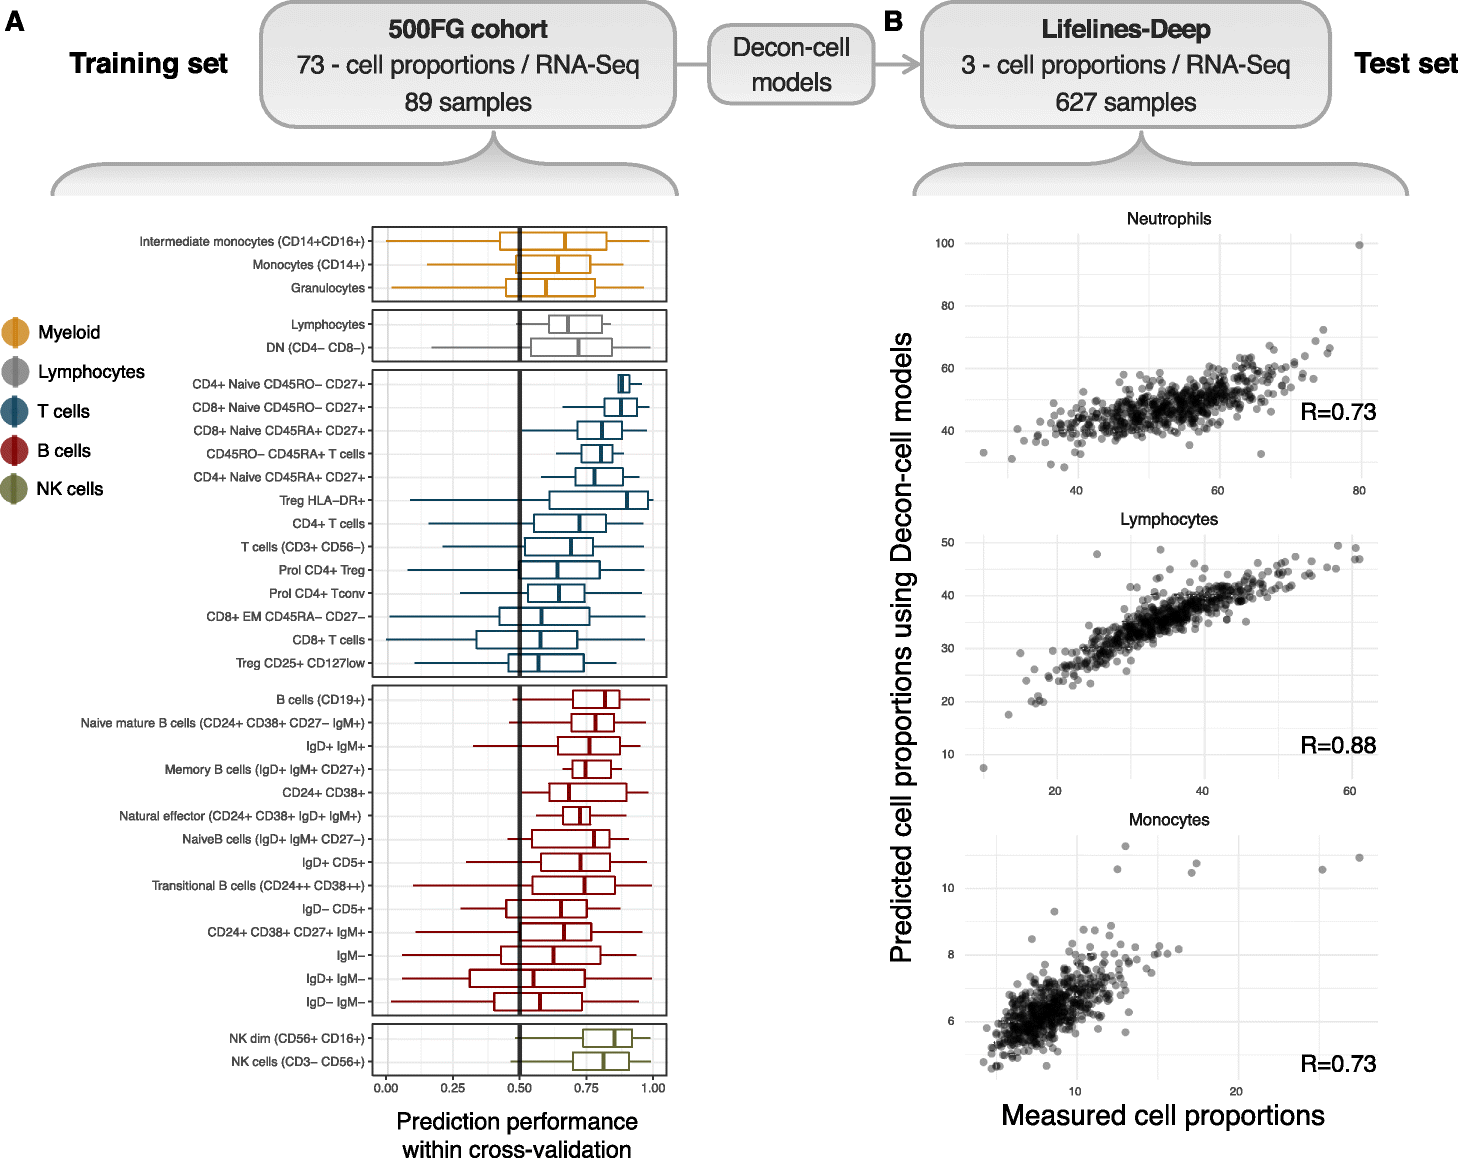
\includegraphics[width=\textwidth]{chapters/chapter4-deconvolution/img/fig2.png}
	\caption{\textbf{Prediction of cell proportions using whole blood transcriptome by Decon-cell.} (A) Distribution of prediction performance (Spearman correlation coefficient) of the 34 predictable cell types in 100 iterations of prediction within the 500FG cohort. (B) Cross-cohort validation in an independent Lifelines-Deep cohort (n = 627): the measured and predicted cell proportions for neutrophils (given by granulocytes in 500FG), lymphocytes and monocytes are compared}
	\label{decon_fig2}
\end{figure}


\Needspace{10\baselineskip}
\subsection{Decon-eQTL identifies which cell types contribute to the whole blood eQTL effect}
As we know, eQTL analysis using whole blood bulk expression data fails to distinguish between a general eQTL that is present in all cell types and an effect that is mainly found in a subset of the cell types. We therefore propose a new approach to assign the overall bulk eQTL into CT effects, called Decon-eQTL (see Online Methods). By using the cell proportions in whole blood, it is possible to formally test if the genetic effect is interacting with the cell proportions. More explicitly, we include both the genotype and all major CT proportions of interest in a linear model and systematically test if there is a significant interaction effect between genotype and each of the cell proportions in the variation of gene expression in whole blood. At the same time the model used by Decon-eQTL controls the effect of the remaining cell types on gene expression. In this way, whole blood expression data, alongside genotypes and (predicted) cell proportions can be integrated to assign a CTi effect from a bulk eQTL(\textbf{Figure \ref{decon_fig1}}).

We applied Decon-eQTL to 3,198 samples (BIOS cohort) with transcriptome levels (RNA-seq), genotype information and cell proportions predicted by Decon-cell. Whole blood cis-eQTL mapping yielded 16,362 whole blood eQTLs (false discovery rate (FDR) $\leq 0.05$). For each of these whole blood cis-eQTLs, we applied Decon-eQTL with a focus on 6 major cell sub-populations: granulocytes, CD14+ monocytes, CD4+ T-cells, CD8+ T-cells, B-cells and NK cells. These cell types were selected as the sum of their relative percentages was close to 100\% and none of these cell type pairs had an absolute correlation coefficient $R \geq 0.75$. Decon-eQTL computationally assigned 4,139 CTi eQTLs from these sub-populations, reflecting 3,812 genes and 3,650 SNPs. 25\% of the whole blood eQTLs have a significant ($FDR \leq 0.05$) CTi eQTL effect given Decon-eQTL. The majority (31\%) of the total CTi eQTL effects detected were found to be associated to granulocyte proportions, possibly because granulocytes comprise ~70\% of circulating white blood cells (\textbf{Figure \ref{decon_fig3}A}). The majority (74\%) of CTi eQTLs detected by our method were assigned to a single cell type (\textbf{Supplementary Figure 6A}), similarly we find almost no sharing between cell types in single cell eQTLs from 112 individuals. However, it should be noted that these eQTL are likely not exclusively present for this particular cell type in biology, but that the statistical power given our sample size was sufficient to detect these interaction effects which we describe as CTi eQTL, in this particular cell type . Decon-eQTL was only able to find sharing of CTi eQTLs between cell types in a few cases, likely due to a lack of power of the interaction model. An example of such shared CTi eQTLs is on NOD2 gene, where Decon-eQTL was able to detect a strong granulocyte-eQTL effect alongside a smaller, opposite effect in CD14+ monocytes. This opposite effect has also been previously described in eQTL studies on purified CD14+ monocytes and neutrophils8. These results demonstrate that the effects of cell proportions on gene expression should be taken into account when interpreting eQTLs derived from bulk tissues.

\begin{figure}[H]
	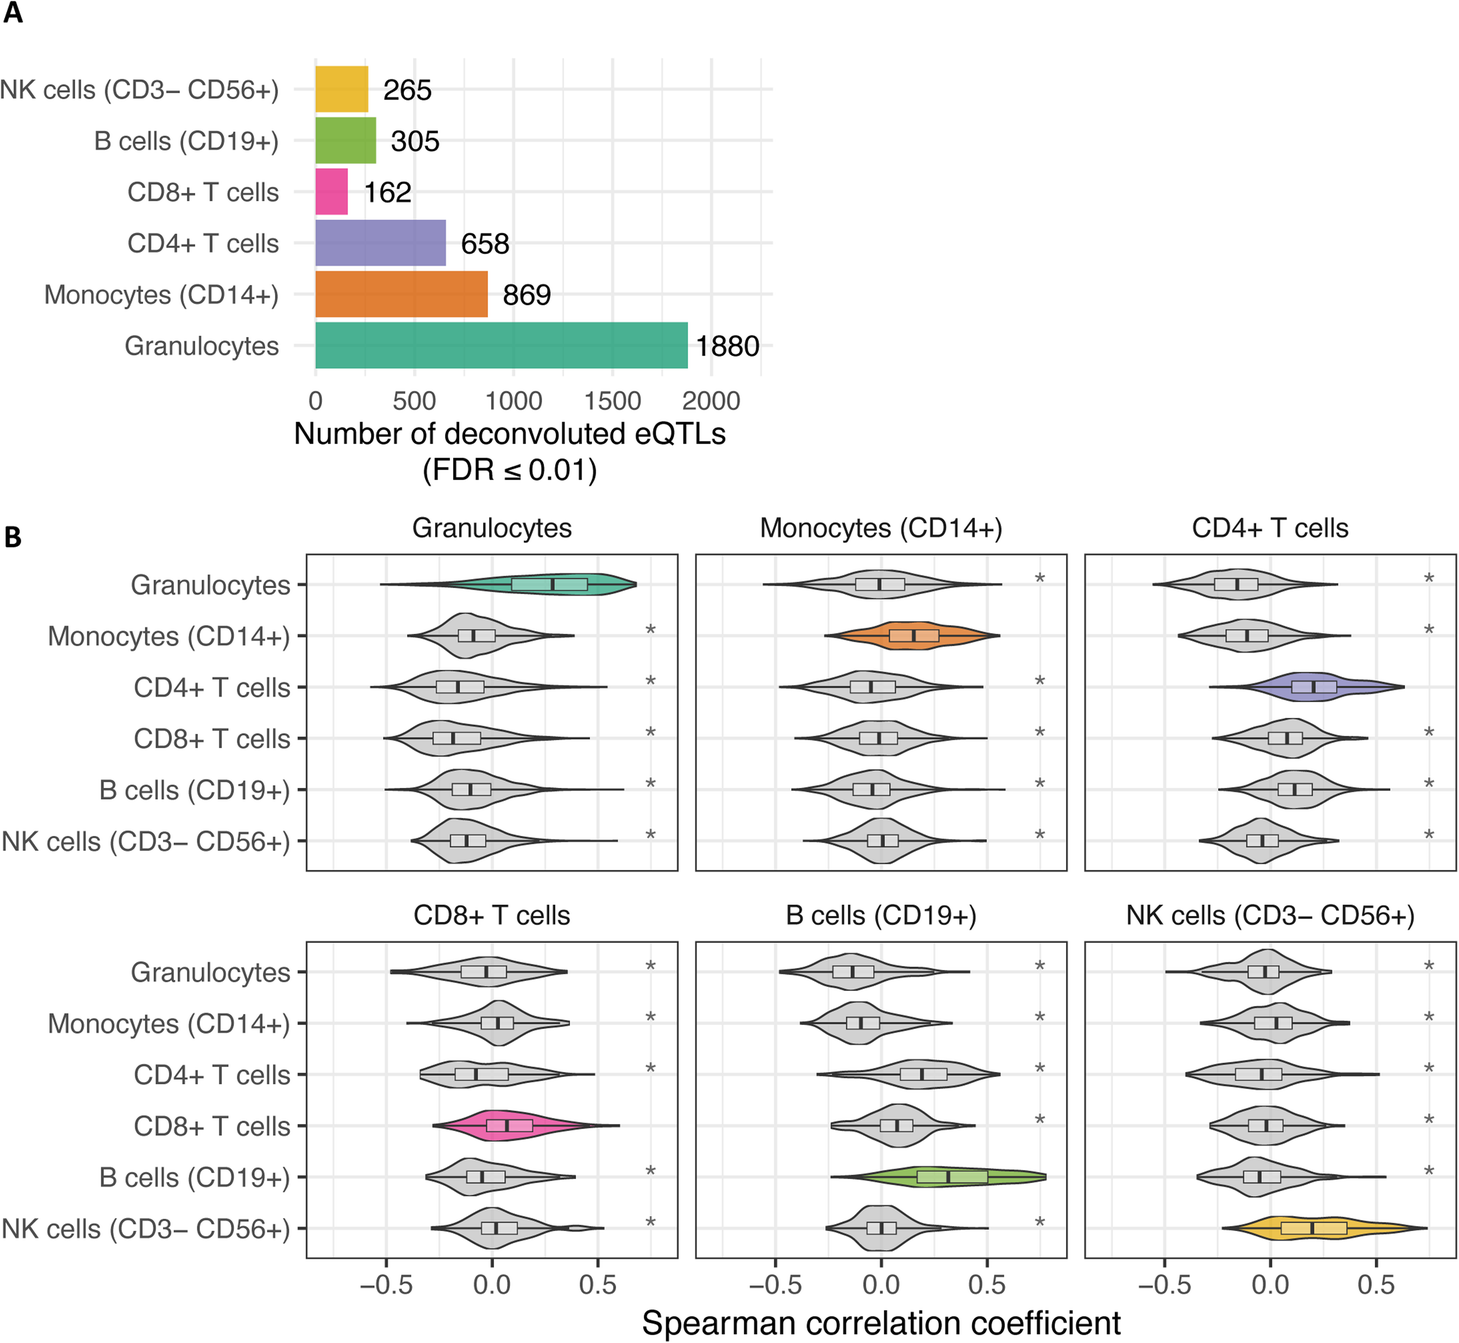
\includegraphics[width=\textwidth]{chapters/chapter4-deconvolution/img/fig3.png}
	\caption{\textbf{Deconvolution of whole blood eQTLs into CTi eQTLs}. Decon-eQTL detects CTi eQTLs by integrating proportions of cell subpopulations (predicted by Decon-cell), gene expression and genotype information. (A) Number of deconvoluted CTi eQTLs in each cell type using whole blood RNA-seq data of 3189 samples in BIOS cohort. (B) Distribution of Spearman correlation coefficients between expression levels of CTi eQTL genes and cell counts for each cell subpopulation. The CTi eQTL genes show positive and statistically higher correlation (Spearman) with the relevant cell type proportions as compared to the rest (T-test p-value $<$ 0.05) in an independent cohort (500FG)}
	\label{decon_fig3}
\end{figure}


\Needspace{10\baselineskip}
\subsection{Decon-eQTL prioritizes genes to relevant cell types}
CTi eQTL genes are expected to have higher expression levels in their relevant cell types and therefore, their expression in whole blood should be correlated with the proportions of its given cell type. To test this, we evaluated if the expression levels of the CTi eQTL genes detected in the BIOS cohort were correlated with their relevant cell proportions and compared this to the correlation with non-relevant cell types. We calculated the Spearman correlation coefficients between the expression of the identified CTi eQTL genes and the measured cell proportions using the 500FG cohort ($n = 89$). Next, we compared the correlation coefficients obtained with those between expression and the remaining cell proportions. For each of the six evaluated cell sub-populations in Decon-eQTL, CTi eQTL genes had a significantly higher correlation with their relevant cell subpopulation than the other cell types (T test, p-value $\leq 0.05$) (\textbf{Figure \ref{decon_fig3}B}). As such, this result shows a significant association CTi eQTL ytgenes and the proportions of their relevant CT in an independent cohort.

Next, we evaluated whether the significant CT eQTL genes were over-expressed in their relevant cell subpopulation compared to eQTL genes that were found to be non-significant CTi eQTLs for the same cell type. For this purpose, we made use of the purified neutrophil, CD14+ monocyte, CD4+ T-cell and B-cell RNA-seq data from the BLUEPRINT dataset. We only include these cell types as they were the only ones with more than 3 samples measured. For each of the four cell types, we observed that the expression of CT eQTL genes detected by Decon-eQTL was significantly higher (T-test, p-value $\leq 0.05$) compared to the expression of non-significant Decon-eQTL genes (\textbf{Figure \ref{decon_fig4}A}). We also observed that the deconvoluted eQTL genes from granulocytes showed a relatively wider range of variation than the CT-eQTL genes from the other three sub-populations. We hypothesized that this could be explained by the fact that granulocytes comprise ~70\% of the cell composition in whole blood, thus giving us the power to detect eQTL for lowly-expressed genes in granulocytes. This was partly supported by the observation that the variation of expression in whole blood for granulocyte CTi eQTL genes was significantly greater than those CTi eQTL genes deconvoluted to the other five cell sub-populations (F test, p-value $\leq 0.05$, \textbf{Supplementary Figure 7}). 

Furthermore, by using publicly available transcriptome profiles (GSE7884027) of purified NK cells and CD4+ T cells, we assessed if the differentially expressed genes across the two cell types were enriched for eGenes of deconvoluted CT eQTLs. We observed that the CD4+ differentially expressed genes (Adjusted p-value $\leq 0.05$) were significantly enriched for CD4+ T cell eQTLs (Fisher exact p = $1.8 \times 10^{-17}$), whereas NK cell differential genes (Adjusted p-value $\leq 0.05$) were significantly enriched for NK cell eQTLs (Fisher exact p = $2.3 \times 10^{-18})$ as shown in \textbf{Figure \ref{decon_fig4}B}.

In summary, we were able to show that the eQTL genes detected by Decon-eQTL are transcriptionally active in their relevant cell type as that is where they are more highly expressed.

\begin{figure}[H]
	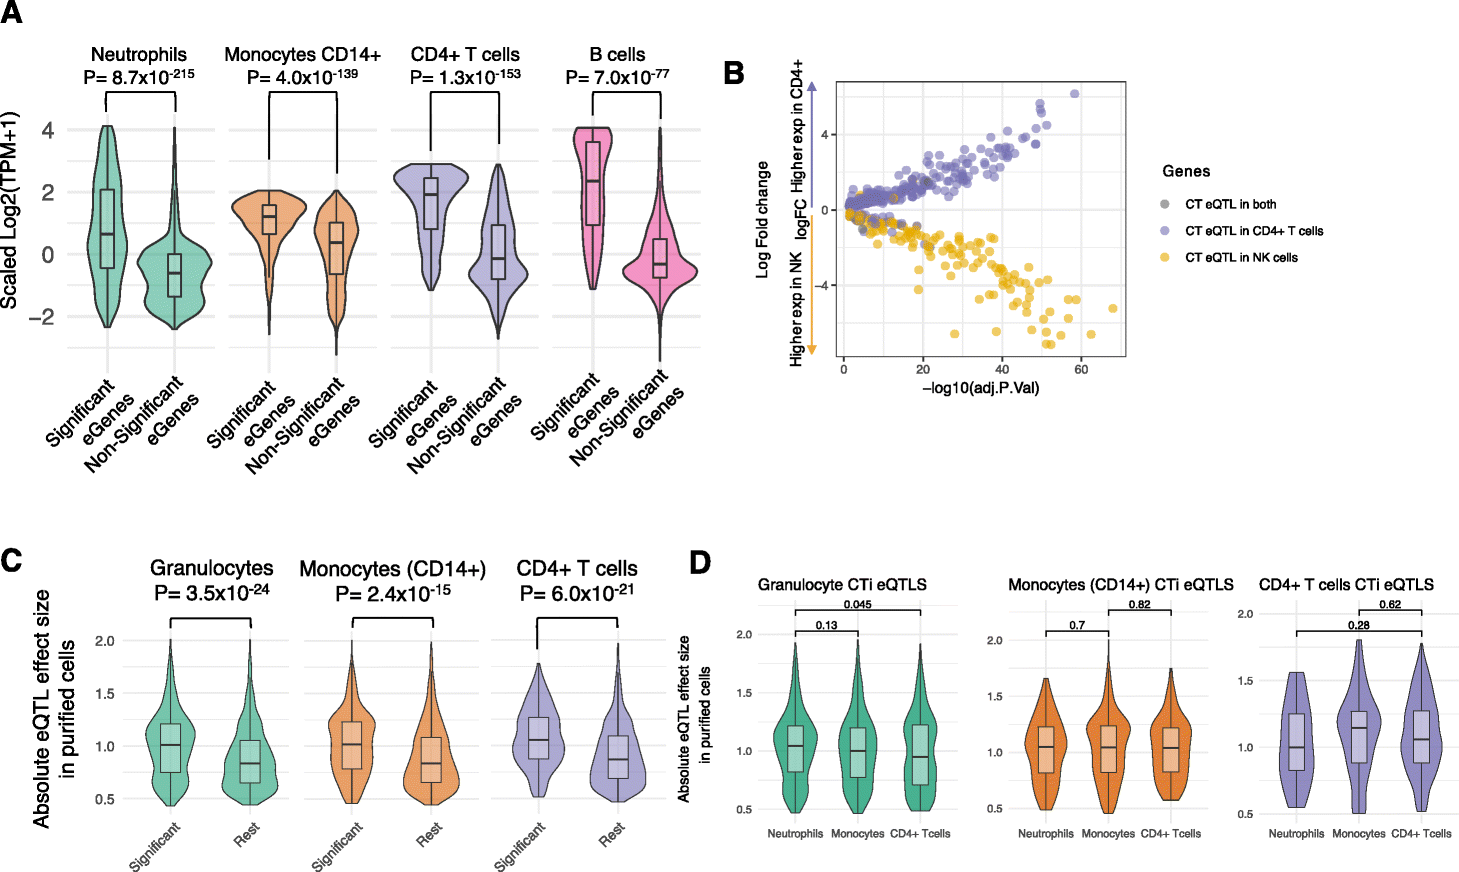
\includegraphics[width=\textwidth]{chapters/chapter4-deconvolution/img/fig4.png}
	\caption{\textbf{Validation of CTi eQTLs.} (A) The expression of CTi eQTL genes in purified cell subpopulations from BLUEPRINT\cite{adamsBLUEPRINTDecodeEpigenetic2012} are significantly higher in the relevant cell subpopulation when compared to other available cell subtypes (green for granulocyte eQTL genes showing expression for purified neutrophils; orange for monocytes; purple for CD4+ T cells; pink for B cells). (B) Genes differentially expressed (Adjusted p-value $\leq$ 0.5) between CD4+ T cells and NK cells are significantly enriched for CT eQTLs effects on CD4+ T cells (dots in purple, Fisher exact $-log_{10}(p) = 1.8 \times 10^{17}$) and NK cells (dots in yellow, Fisher exact $-log_{10}(p) = 2.3 \times 10^{18}$), respectively. (C) CTi-eQTLs (FDR $\leq$ 0.05) show significantly larger effect sizes in the purified cell eQTL data\cite{chenGeneticDriversEpigenetic2016} compared to the rest of the whole blood eQTLs for which we do not detect a cell type effect, as shown for deconvoluted granulocyte eQTLs in neutrophil-derived eQTLs (green),monocytes (orange) and CD4+ T cells (purple)}
	\label{decon_fig4}
\end{figure}


\Needspace{10\baselineskip}
\subsection{CT eQTLs identified by Decon-eQTL in whole blood are replicated in purified cell eQTL datasets}
In order to validate the CT eQTLs defined by decon-eQTL, we utilized the eQTLs identified from purified neutrophils, CD4+ T-cells and CD14+ monocytes\cite{chenGeneticDriversEpigenetic2016}. We first compared the absolute effect sizes of eQTLs from purified cells that are also significantly deconvoluted CTi eQTLs with the effect sizes of eQTLs from purified cells that are also non-significant deconvoluted CTi eQTLs for this cell type. For all three cell populations, effect sizes in our deconvoluted CTi eQTLs were significantly higher compared to the effect size of eQTLs without a significant CTi eQTL (Wilcoxon test, p-value $\leq 0.05$, \textbf{Figure \ref{decon_fig4}C}). Next, we assessed the specificity of our deconvoluted CTi eQTLs by evaluating CTi eQTL effect sizes in non-relevant cell sub-populations. For example, we compared the effect sizes of deconvoluted granulocyte CTi eQTLs against those with non-significant deconvoluted granulocyte CTi eQTLs using the effect sizes of purified CD4+ T-cell eQTLs. Notably, we observed no statistically significant differences using effect sizes from non-relevant cell sub-populations (see off-diagonal comparisons in \textbf{Supplementary Figure 8}), further supporting the biological relevance of our deconvoluted CTi eQTLs. However, when comparing the effect sizes in purified eQTLs of only significant CTi eQTLs across all three available cell sub-populations, we were not able to find significant differences (\textbf{Figure \ref{decon_fig4}D}). For example, the effect size of neutrophils CTi eQTLs is the same across neutrophils, monocytes CD14+ and CD4+ T cells.

To further demonstrate that the CTi eQTLs assigned by Decon-eQTL are biologically meaningful, we have made use of the K27AC and K4ME1 epigenetic QTLs characterized in purified neutrophils, CD4+ T-cells and monocytes CD14+\cite{chenGeneticDriversEpigenetic2016}. In a similar fashion as the above comparison of effect sizes with purified eQTLs, we compared the absolute effect sizes from both K27AC and K4ME1 QTLs from eQTLs for which Decon-eQTL detects a significant CTi effect against the rest of whole blood eQTLs. We observed that for corresponding cell types, e.g. evaluating granulocyte CT eQTLs in K27AC QTLs from purified Neutrophils, the distribution of the absolute effect sizes is significantly higher for the chromatin mark QTLs (cmQTLs) than those non-significant CT eQTLs, which provide an epigenetic evidence that  our method is able to assign correctly the cell type eQTL effects, as shown in the diagonal comparisons in both K27AC QTLS (\textbf{Supplementary Figure 9}) and for K4ME1 QTLs (\textbf{Supplementary Figure10}). Notably, we observed that for the non-relevant cell sub-populations only one comparison, i.e. granulocytes v.s. CD14+ monocytes, show statistically significant higher effect sizes for K27AC QTLs and K4ME1 QTLs. For the rest of the non-relevant comparisons in the off-diagonal of both \textbf{Supplementary Figure 9} and \textbf{Supplementary Figure 10}, there are no statistically significant differences. Comparing the eQTL effect sizes in purified KC27AC and K4ME1 QTLs of only significant CTi eQTLs across all three available cell sub-populations shows that the effect sizes from the relevant cell type are  significantly stronger for all pairings except between granulocytes and CD14+ monocytes (\textbf{Supplementary Figure 11}).

In addition to the comparison of effect sizes, we compared the allelic concordance between deconvoluted eQTLs and eQTLs from purified cell subtypes9. For each available cell type (neutrophils, CD14+ monocytes, and CD4+ T cells), we evaluated whether the direction of the eQTL effect on deconvoluted CT eQTLs was the same as the one observed from purified cell sub-populations. The allelic concordance between the deconvoluted eQTLs and purified eQTLs was high across cell types: 99\% for granulocyte eQTLs (compared to neutrophil eQTLs), 96\% for CD14+ monocytes eQTLs, and 99\% for CD4+ T cells (\textbf{Figure \ref{decon_fig5}A}). These rates of allelic concordance are significantly higher for granulocyte and CD4+ T-cell CTi eQTLs compared to those between whole blood eQTLs and eQTLs from purified cell sub-populations (\textbf{Figure \ref{decon_fig5}B}, Neutrophils, Fisher exact p-value = $3.91 \times 10^{-106}$, CD4+ T cells Fisher exact p-value = $0.005$),  whereas the allelic concordance for deconvoluted CD14+ monocyte eQTLs is the same as for whole blood eQTLs and purified CD14+ monocyte eQTLs (\textbf{Figure \ref{decon_fig5}B}). We also compared the allelic concordance of deconvoluted CTi eQTLs of a certain cell type against the eQTLs of non-relevant purified sub-populations. Interestingly, the allelic concordance across non-relevant cell subtypes is consistently lower (off-diagonal \textbf{Supplementary Figure 12}, bonferroni corrected fisher exact p-value $< 0.0001$ for all comparisons). The higher allelic concordance across cell types was seen between deconvoluted granulocyte eQTLs and CD14+ monocyte eQTLs with a 95\% allelic concordance, which shows that the direction of effect is often shared between related cell types.

\begin{figure}[H]
	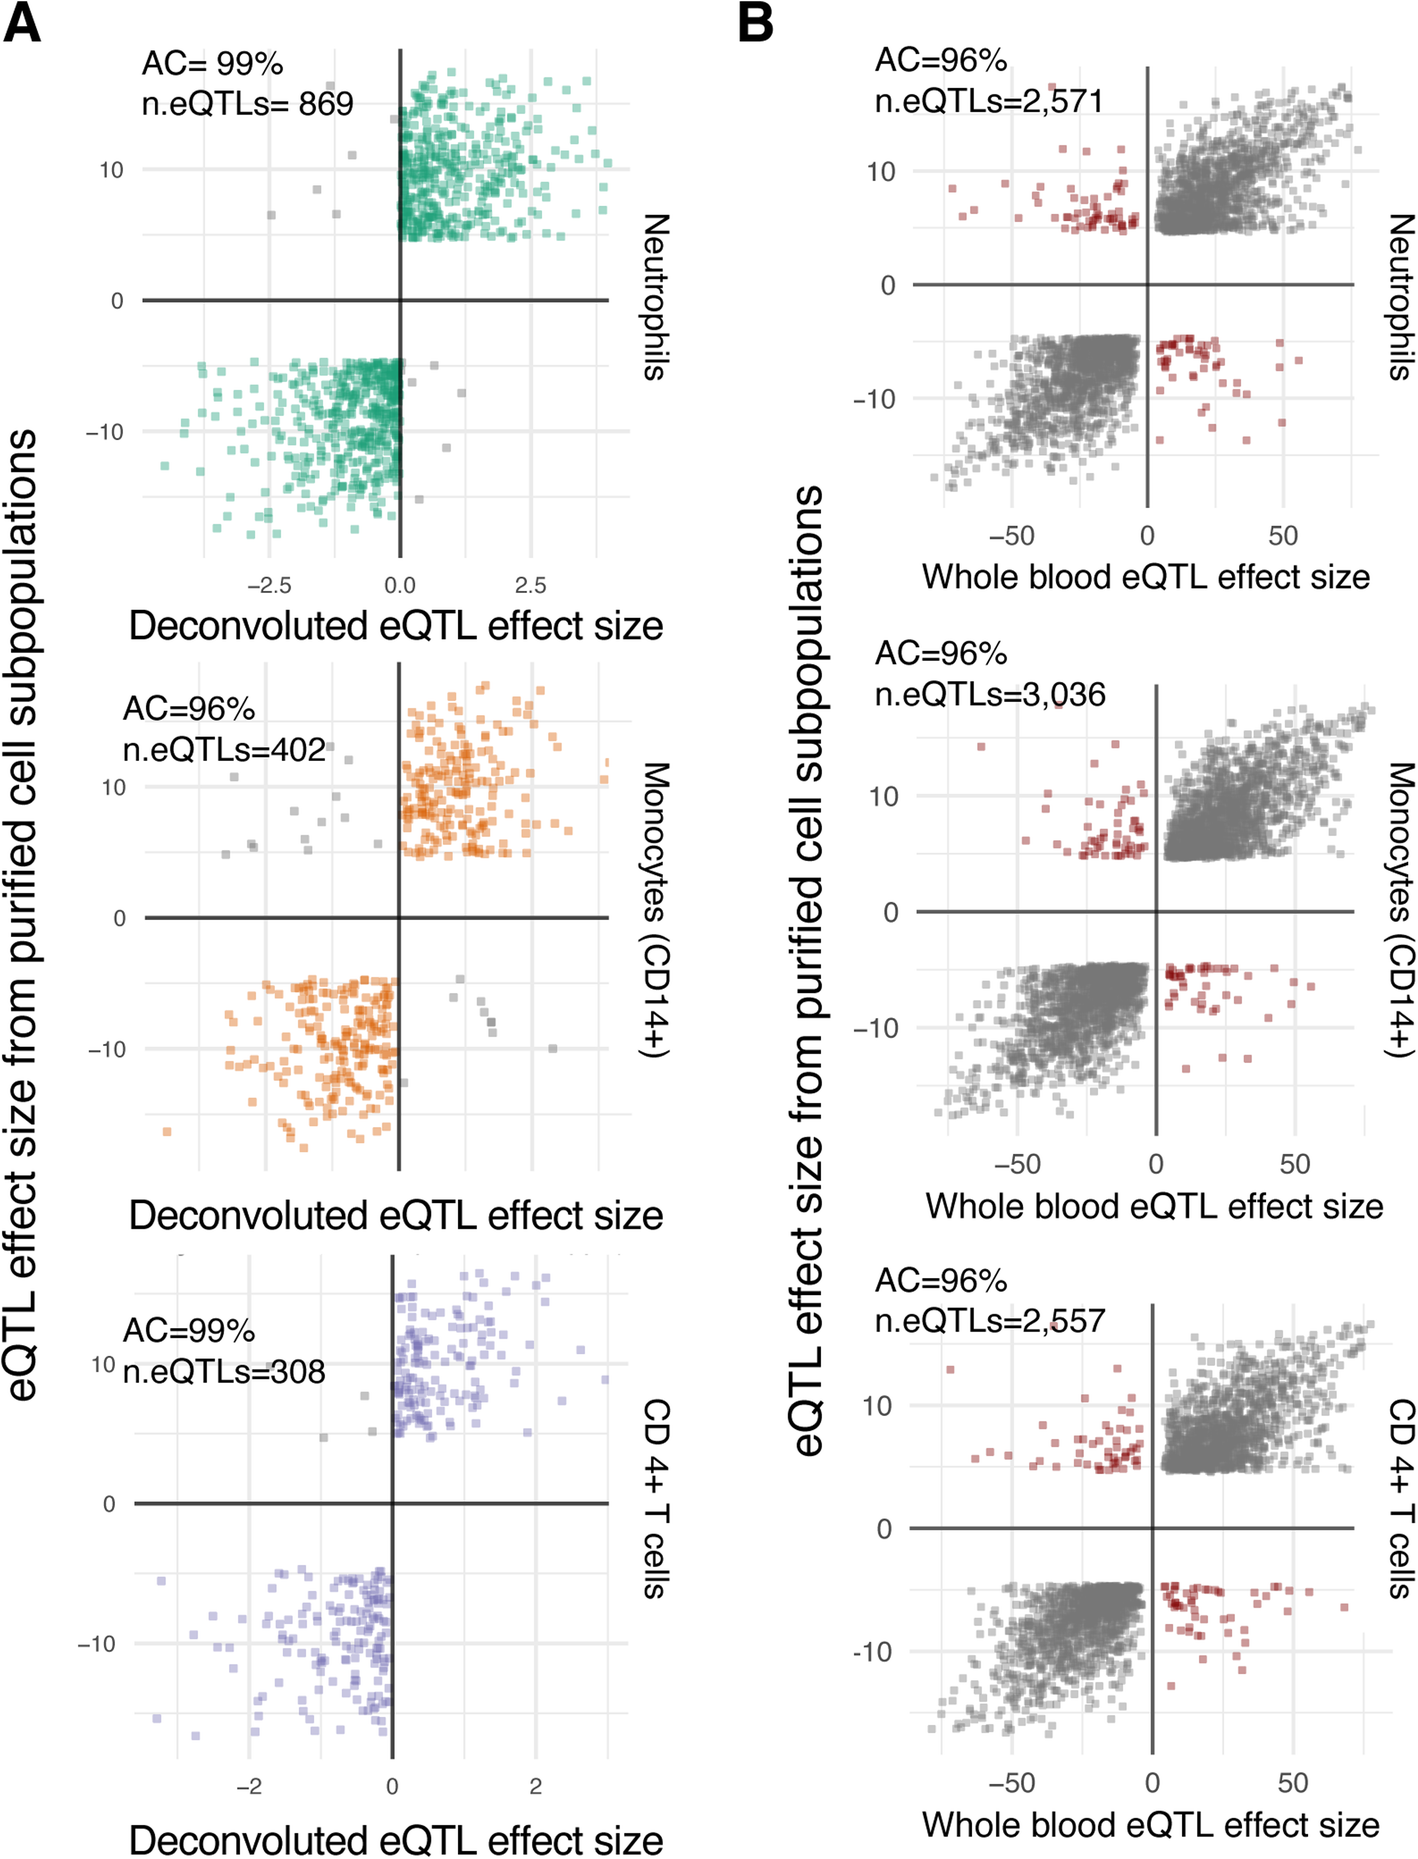
\includegraphics[width=\textwidth]{chapters/chapter4-deconvolution/img/fig5.png}
	\caption{\textbf{Allelic concordance of CTi eQTLs with eQTLs from purified cells.} CTi eQTLs show high allelic concordance compared to eQTLs from purified cell subpopulations9. (A) for granulocyte eQTLs (green), CTi eQTLs achieved an allelic concordance of 99\% compared to eQTLs from purified neutrophils. Similarly, the allelic concordances were 96 and 99\% for CD14+ monocytes and CD4+ T cells, respectively. Except for monocytes, these values are higher than those observed for whole blood eQTLs when comparing to eQTLs from purified subpopulations, as shown in panel (B)}
	\label{decon_fig5}
\end{figure}

Finally, we evaluated the allelic concordance rates for CTi eQTLs assigned by Decon-eQTL and K27AC QTLs from purified cell sub-populations, where we observed a consistently high allelic concordance rate: 92\% for granulocyte eQTLs (in purified Neutrophils), 87\% for CD14+ monocytes and 92\% for CD4+ T cells (boxed diagonal comparisons in \textbf{Supplementary Figure 13}). These concordance rates are significantly higher than the ones between the whole blood eQTLs and K27AC QTLs from purified cell sub-populations (\textbf{Supplementary Figure 14}) for neutrophils (Fisher exact test p-value $= 9.06 \times 10^{-14}$), CD14+ monocytes (Fisher exact test p-value $= 3.33 \times 10{-4}$), CD4+ T cells (Fisher exact test p-value $= 8.64 \times 10^{-9}$). Moreover we notice a consistent decrease in allelic concordance rates when assessing the concordance of CT eQTLs in K27AC QTLs of non-relevant cell sub-populations (off-diagonal compasons, \textbf{Supplementary Figure 13}). Together, the results from allelic concordance rates between deconvoluted CTi eQTLs and eQTLs/K27AC QTLs from purified cell sub-populations add a further layer of evidence supporting the biological relevance of deconvoluted CT eQTLs.

\Needspace{10\baselineskip}
\subsection{CTi eQTLs identified by Decon-eQTL in whole blood show high allelic concordance with single-cell RNA-seq eQTLs}
To replicate the deconvoluted CT eQTLs in the cell subtypes that were not available in Chen \textit{et al.}\cite{chenGeneticDriversEpigenetic2016}. purified cell eQTLs, we utilized the recent single-cell RNA-seq eQTLs (sc-eQTLs) identified in CD14+ monocytes, NK cells, CD4+ T-cells, CD8+ T-cells, and B-cells\cite{wijstSinglecellRNASequencing2018} as well as new single cell data eQTL data that was processed in the same way. Combined, we used single cell eQTLs from 112 individuals. We selected all significant eQTLs for each of the cell types (Non Classical and Classical Monocytes were combined) and compared it to the direction of the eQTL effect given by Decon-eQTL. Overall we observed an allelic concordance of 96.42\% (\textbf{Figure \ref{decon_fig6}A}).

\Needspace{10\baselineskip}
\subsection{Decon-QTL outperforms conventional interaction method}
To our knowledge, our approach is the first to model the effect of multiple components of bulk blood RNA-seq simultaneously in an attempt to fully deconvolute gene expression levels into more precise cell type x genotype effects. Previous studies used an interaction effect between genotype and cell proportions of one specific cell type to detect the cell type eQTL effects using whole blood gene expression\cite{westraCellSpecificEQTL2015}, or used the correlation of the eQTL effect with cell type proxy genes\cite{zhernakovaIdentificationContextdependentExpression2017}. 

The Westra et al method has often been used to detect cell type eQTL effects using bulk expression data and cell proportions\cite{davenportDiscoveringVivoCytokineeQTL2018,wilsonMappingTumorSpecificExpression2019,geeleherCancerExpressionQuantitative2018,glastonburyCellTypeHeterogeneityAdipose2019}. In brief, it focuses on the effect of the GxE interaction (where E represents cell proportions) for explaining the variation in gene expression, and it only incorporates one cell type at a time. To properly compare Decon-eQTL with the Westra \textit{et al.} method\cite{westraCellSpecificEQTL2015}, coined here ‘Westra method’, both methods were applied to the BIOS cohort, where we detected CT eQTLs for the six cell sub-populations. Replication of CT eQTLs from Westra method was done in the same way as described above for Decon-eQTL. We observed that the eGenes (i.e. genes with eQTLs) detected by the Westra method are significantly higher expressed for granulocytes ($p = 3.0 \times 10^{-12}$, observed in purified neutrophils), CD4+ T cells ($p = 5.0 \times 10^{-13}$) and B cells ($p = 5.1 \times 10^{-11}$), but not for CD14+ monocytes ($p = 1$, see \textbf{Supplementary Figure 15A}). Next, we found that the distribution of effect sizes in eQTLs from purified cells is significantly higher for the CT eQTLs detected using the Westra et al method when compared to the rest of the whole blood eQTLs ($p = 2.2 \times 10^{-47}$, $p = 9.6 \times 10^{-08}$, $p = 1 \times 10^{-47}$ for Neutrophils, Monocytes and CD4+ T cells respectively, boxed-diagonal comparisons in \textbf{Supplementary Figure 15B}) showing similar results as the ones from Decon-eQTL (\textbf{Supplementary Figure 8}).

When comparing the allelic concordance rates between the direction of effects given by the interaction term from the Westra method and those found in eQTLs from purified cell sub-populations, we observed that the allelic concordance for granulocytes eQTLs (99\%, evaluated in neutrophils, $p > 0.05$) and for CD4+ T cells 93\% (p $>$ 0.05), \textbf{Supplementary Figure 17}) is comparable to those observed for Decon-eQTL (\textbf{Figure \ref{decon_fig4}A}). Conversely, the allelic concordance rate for the CD14+ monocytes is only 62\%, significantly lower than the results from Decon-eQTL(96\%, $p = 0.001$). Finally, for granulocytes, CD4+ T cell eQTLs and monocytes, we have overlapped the the results from Westra method and Decon-eQTL with the eQTLs from purified cell types\cite{chenGeneticDriversEpigenetic2016} (\textbf{Supplementary Figure 17}). For all three cell types, we found that Decon-eQTL is able to detect a larger number of eQTLs. For Neutrophils the Westra method has a higher replication rate (fisher $p-value = 0.002$), for monocytes the methods had the same replication rate (fisher p-value $= 0.737$), and for CD4+ T-cells Decon-eQTL had a better replication rate (p-value $= 7.47 \times 10^{-12}$). 

Finally, we compare the difference in allelic concordance with single cell eQTLs. The overall allelic concordance of Decon-eQTL CTi QTLs with single cell eQTLs (96.42\%, Fig 6A) is higher than the one achieved by the Westra model ($p = 1.235 \times 10^{-08}$), where we observed an overall allelic concordance of 84.67\% (Fig 6B). For both non-classical Monocytes (fisher p-value $= 0.045$) and CD4+ T-cells (fisher p-value $= 7.896 \times 10^{-07}$) Decon-eQTL has a significantly better allelic concordance, for CD8+ T-cells (fisher p-value $= 0.230$), classical Monocytes (fisher p-value $= 0.0513$), B-cells (fisher p-value $= 0.055$) and NK cells (fisher p-value $= 0.242$) there is no significant difference, nevertheless for NK cells, classical Monocytes, and CD8+ T cells, Decon-eQTL show a higher allelic concordance (93.8\% vs 83.9\%, 96.2\% vs 89.2\%, and 100\% vs 93.5\% respectively), while for B-cells it has lower concordance (33\% vs 100\%, \textbf{Figure \ref{decon_fig6}B}).

Overall, these results demonstrate that Decon-eQTL is able to detect more CTi eQTLs that can be replicated in purified eQTL dataset that previously reported methods, especially in not so abundant cell types such as CD14+ monocytes. However, the detection of interaction effects between genotype and cell proportions to dissect bulk (in this case whole blood) expression data and detect CTi eQTLs, remains an area of great opportunity that could still be explored. Mainly to the constantly increasing  number of samples present in functional genomic cohorts and the greater number of purified and single cell eQTL dataset that can be used for validation. 

\begin{figure}[H]
	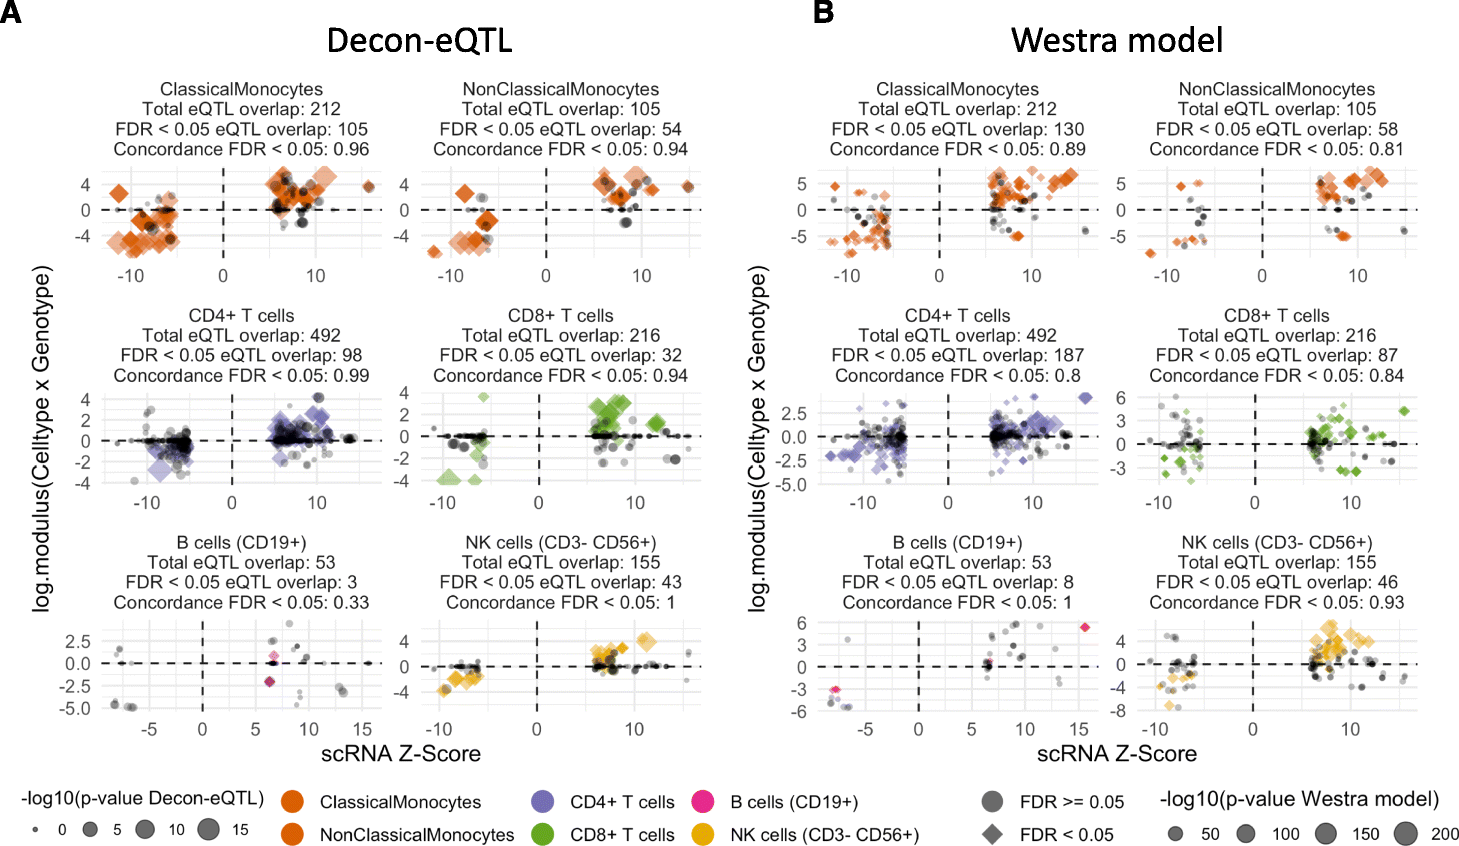
\includegraphics[width=\textwidth]{chapters/chapter4-deconvolution/img/fig6.png}
	\caption{\textbf{Allelic concordance of CTi eQTLs with eQTLs from single cell RNAseq.} (A) Comparison in allelic direction between CTi eQTLs and eQTLs from single cell RNAseq experiments in 6 cell types. (B) Comparison in allelic direction between Westra model eQTLs and single cell eQTLs. In both panels coloured diamonds are FDR $<$ 0.05, grey circles are FDR $geq$ 0.0 in the single cell data, and the size is the $-log_{10}(p-value)$ of the predicted cell type interacting eQTLs}
	\label{decon_fig6}
\end{figure}

\Needspace{10\baselineskip}
\section{Discussion}
We have developed a novel statistical framework, Decon2, which predicts the proportions of known immune cell subtypes using gene expression levels from whole blood (Decon-cell). Subsequently, these predicted cell proportions, together with genotype information and expression data, can be used to deconvolute a whole blood  eQTL effect into cell type interacting effects (Decon-eQTL). Using a set of samples with both whole blood RNA-seq data and cell frequencies of 73 cell sub-populations, we demonstrated that Decon-cell was able to predict 34 independent cell sub-populations. The performance of Decon-cell has been validated using multiple independent cohorts and benchmarked with existing methods. The obtained Decon-cell models were applied to a cohort of 3,189 samples with whole blood RNA-seq available, resulting in predicted cell counts for these samples. By integrating bulk expression data, genotype and predicted cell counts of BIOS cohort,  Decon-eQTL was able to dissect whole blood eQTL effect into CTi eQTLs without purifying immune cell sub-populations. Again the results of Decon-eQTL were validated by using several independent data types: 1) eQTLs from purified cell sub-populations, 2) chromatin QTLs purified cells 3) gene expression from purified cell types and 4) eQTLs derived from single cell protocols. Compared with existing methods, Decon-eQTL consistently show superior performance. To sum up, the proposed framework is useful for (re)-analyse both, existing and new bulk blood tissue datasets to detect CTi eQTL effects, and can be applied and tested on other tissues once cell count proportions become available. This cataloging and further interpreting the role of CTi eQTLs will improve our understanding of the functional role of SNPs associated with complex diseases, at the level of specific cell subtypes.

The main advantage of our method for predicting cell proportions by Decon-cell  is that it does not rely on the gene expression measured in purified cell subtypes when defining signature gene sets. Moreover, our method does not require the definition of marker genes based on their differential expression compared to other cell sub-populations unlike previously reported methods\cite{aranXCellDigitallyPortraying2017}. The signature genes defined by Decon-cell are determined by a completely unsupervised approach using a regularized regression to select an optimal combination of genes to accurately predict a certain circulating cell proportion. Although the majority of these marker genes are differentially expressed across purified cell sub-populations, not all of them are. Nevertheless, these signature gene sets are still correlated to the cell proportions in whole blood. In summary, we have shown that Decon-cell is able to accurately predict the proportions of circulating immune cell sub-populations in three independent cohorts and that within these cohorts it out-performs previously reported methods.

Our Decon-eQTL method for detecting a CTi eQTL effect with bulk blood tissue expression data is, to our knowledge, the first attempt to simultaneously model whole blood gene expression profiles into its major components. In contrast to a previous method, where single cell type  ($G \times E$) effects were evaluated one at a time\cite{westraCellSpecificEQTL2015,glastonburyCellTypeHeterogeneityAdipose2019}, Decon-eQTL incorporates all the major cell proportions simultaneously to better dissect the overall genetic effect of gene expression signal into cell subpopulation effects. We have shown that CTi eQTL genes found with Decon-eQTL have higher expression and higher effect sizes in purified neutrophils, CD14+ monocytes and CD4+ T-cells than non-CTi genes, and we find significantly higher allelic concordance for 2 out of 4 tested cell types with single cell eQTLs than with a conventional interaction model (Fig 6A and 6B). Moreover, we have also shown the biological relevance of the deconvoluted CTi eQTLs by validating our results on cmQTLs where CTi eQTLs have significantly higher effect sizes and its allelic concordance rates are significantly higher than those of whole blood eQTLs.  Finally, we have also demonstrated that Decon-eQTL can replicate sc eQTLs derived from single-cell RNA-seq data, showing a higher allelic concordance with sc-eQTLs compared to using only whole blood eQTL effects.

There are limitations in our method: the CTi eQTLs detected by Decon-eQTL tend to be exclusive eQTL for the specific CT suggesting that the CT with the strongest eQTL effect was selected by Decon-eQTL. This is  likely due to the partial collinearity present between CT proportions included in the model (as shown by their correlation structure in \textbf{Supplementary Figure 18A-B}). Thus, the genetic effect of one cell type might be masked by another CT with correlated cell proportion. The highest correlation coefficient among cell types included in the model was 0.75 (between granulocytes and B cells). Therefore, a caveat to this is that by deconvoluting CTi eQTLs for partially correlated cell proportions could lead to false negative results for the cell types with relatively weaker eQTL effects. 
In our model we included the six major blood cell types. There are many more cell types available, for which our method is not able to detect a CTi eQTL estimate. Furthermore, we only tested Decon-eQTL using genome-wide whole blood cis-eQTLs main effects. Such eQTLs effects are very likely shared across multiple cell types, however due to statistical power and co-linearity we are only able to detect its interaction with only one cell type (\textbf{Supplementary Figure 6A}), which is also seen in single cell eQTLs with limited (112) samples (\textbf{Supplementary Figure 6B}). Nevertheless, this does not imply that the CTi eQTL are exclusive for or only present in such cell type, as we observe in \textbf{Figure \ref{decon_fig4}D}, where the effect sizes of the significant CTi eQTLs in purified sub-populations are not significantly different across all three purified cell sub-populations. Yet this difference in effect size of CTi eQTLs between relevant and non-relevant cell types can be seen in histone modification QTLs as shown in \textbf{Supplementary Figure 11}, likely due to the cell type specificity of epigenetic marks. Lastly, Decon2 has only been tested in whole blood where large numbers of samples are available, and therefore it is not known how it will perform in other tissues such as solid like bulk tissues.

The proposed framework of Decon2 is generic for predicting cell sub-populations in bulk tissues (Decon-cell) and re-distribute the overall eQTL effect into cell types (Decon-eQTL). Both methods have been implemented in freely available software. In both an R package and a user interface-based webtool, the models for predicting cell subpopulation in whole blood constructed and validated in this work are provided for people interested in estimating immune cell sub-populations in whole blood in healthy people with western european ethnicity, as our models were built using a Dutch cohort (500FG). 

In summary, Decon2 is a computational method that can accurately assign CT effects in whole blood functional genomic cohorts, which can be applied to any dataset for which genotypes and expression data is available and could potentially aid the understanding of the molecular effects of genetic risk factors associated with complex diseases at the cell subpopulation level. Our method makes it possible to create CT gene regulatory networks that could explain the different effects that each CT has on a complex disease in a cost-efficient way. Since Decon2 only requires  gene expression and genotype information to deconvolute bulk blood eQTLs into CTi eQTLs, it is possible to re-analyze the existing bulk blood RNA-seq data for which genotypes are also available; in this scenario we would use Decon-cell to predict cell proportions in whole blood and obtain CT information on many more eQTLs from an increase in sample size. The methods behind Decon2 can potentially be generalized to use transcriptional profiles derived from any other type of bulk tissue in addition to whole blood, such as biopsies from tumors or other solid tissues implicated in complex disease etiology. However, it has not been tested in other tissues. Our methods can hence aid in the detection of genetic effects on gene expression in rare cell sub-populations in bulk tissues. 

\Needspace{10\baselineskip}
\section{Methods}
\Needspace{10\baselineskip}
\subsection{RNA-seq data collection in 500FG cohort}
We selected a representative subset of 89 samples from the 500 participants of the 500FG cohort, which is part of the Human Functional Genomics Project (HFGP). Our subset was balanced for age and sex given the original distribution in the cohort. RNA was isolated from whole blood and subsequently globin transcripts were filtered by applying the Ambion GLOBINclear kit. The samples were then processed for sequencing using the library preparation kit Illumina TruSeq 2.0. Paired-end sequencing of $2 \times 50-bp$ reads was performed on the Illumina HiSeq 2000 platform. The quality of the raw reads was checked using FastQC (http://www.bioinformatics.babraham.ac.uk/projects/fastqc/). Read alignment was performed with STAR 2.3.032,33, using the human Ensembl GRCh37.75 as reference, whilst the aligned reads were sorted using SAMTools\cite{liSequenceAlignmentMap2009}. Lastly, gene level quantification of the reads was done using HTSeq35.

\Needspace{10\baselineskip}
\subsection{RNA-seq preparation and data processing in the BIOS cohort}
RNA was isolated from whole blood and subsequently globin transcripts were filtered by applying the Ambion GLOBINclear kit. Library preparation was performed using the Illumina TruSeq v2 library preparation kit. Next, Illumina HiSeq 2000 was used for paired-end sequencing of $2 \times 50 bp$ reads while pooling 10 samples per lane and expecting $>$ 15 million read pairs per sample. By using CASAVA read sets were generated, retaining only reads that passed Illumina Chastity Filter for further processing.
Quality control of the reads was evaluated using FastQC (http://www.bioinformatics.babraham.ac.uk/projects/fastqc/). Adaptor sequences were trimmed out using cutadapt (v1.1) using default settings. Low quality ends of reads were removed using Sickle (v1.200) (https://github.com/najoshi/sickle). 
Reads were then aligned using STAR 2.3.0e\cite{dobinSTARUltrafastUniversal2013}. All SNPs present in the Genome of the Netherlands (GoNL) with MAF $\geq 0.01$ were masked from the reads to avoid reference mapping bias. Read pairs with at most eight mismatches and mapping to at most five positions, were used. Quantification of counts per genes was done using Ensembl v.71 annotation (which corresponds to GENCODE v.16).

\Needspace{10\baselineskip}
\subsection{Genotype data of the BIOS cohort}
Genotype information was independently generated by each of the cohorts, further details on data collection and methods used for genotyping can be found in their papers (CODAM\cite{damParentalHistoryDiabetes2001}, LLDeep\cite{tigchelaarCohortProfileLifeLines2015}, LLS\cite{deelenGenomewideAssociationMetaanalysis2014}, RS\cite{hofmanRotterdamStudy20162015} and NTR\cite{willemsenNetherlandsTwinRegister2010})

Genotypes were harmonized to GoNL with Genotype Harmonizer\cite{deelenGenotypeHarmonizerAutomatic2014}  and imputed using IMPUTE2\cite{howieFlexibleAccurateGenotype2009} using GoNL as reference panel. SNPs with an imputation score below 0.5, Hardy-Weinberg equilibrium P value smaller than $1 \times 10^{-4}$, a call rate below 95\% or a MAF smaller than 0.05 were filtered out. For further analysis only eSNPs from whole blood cis-eQTL top effects were subsequently used in Decon-eQTL. 

\Needspace{10\baselineskip}
\subsection{Quantification of cell proportions in 500FG cohort}
The inclusion criteria and further description of the participants of the 500FG cohort can be found at http://www.humanfunctionalgenomics.org. A total of 73 manually annotated immune cell sub-populations were quantified using 10-color flow cytometry. To minimize biological variability, cells were processed immediately after blood sampling and typically analyzed within 2–3 hr. Cell populations were gated manually as previously described\cite{aguirre-gamboaDifferentialEffectsEnvironmental2016}.

\Needspace{10\baselineskip}
\subsection{cis-eQTLs in the BIOS cohort}
For cis-QTL mapping, we tested association between genes and SNPs located within 250 kb of a gene center. SNPs with MAF $\geq 0.01$, call rate = 1 and Hardy–Weinberg equilibrium p-value $\geq 0.0001$ were included. eQTLs were declared to be significant at FDR $< 0.05$. Pre-processing of RNA-seq and QTL mapping was performed using a custom eQTL pipeline which has been previously described\cite{zhernakovaIdentificationContextdependentExpression2017}.

\Needspace{10\baselineskip}
\subsection{Prediction of cell proportions using gene expression levels from bulk tissue (Decon-cell)}
For cell count prediction expression data is TMM normalized, log2(expression+1) transformed, and z-transformed (scaled). We proposed that the abundance of molecular markers such as gene expression could be used as proxies to predict cell proportions. This can be represented as:

\begin{equation}
C_{kj} = \beta_{ki} \cdot Y_{ij} + \epsilon_{kj}
\end{equation}

where expression data is $Y_{ij}$ for genes $i = 1, 2,..., G$, samples $j = 1, 2, ..., N$, cell count data is $C_{kj}$ for sample $j$ in cell type $k (k = 1, 2, ..., K)$, $\beta_{ki}$ represents the coefficients of gene $i$ in determining cell counts of cell type $k$ of a complex tissue, and $\epsilon_{kj}$ is the error term.
In order to select only the most informative genes for predicting cell counts, we implemented a feature selection scheme by applying an elastic net (EN) regularized regression25. In the EN algorithm, the $\beta_{ki} \cdot Y$ are estimated by minimizing:

\begin{equation}
\Vert C_{k}-\beta_{k} Y\Vert^2\ subject\ to\ (1 - \alpha) \Vert \beta_{k} \Vert^2 + \alpha \Vert \beta_{k} \Vert_{1} \leq  s
\end{equation}

$s$ is a tuning parameter that limits the number of features that will be included in the final predictor model. We estimate the best s per cell type by applying a 10-fold cross-validation approach, where the most optimal penalty parameter ($\alpha$) was obtained.

\Needspace{10\baselineskip}
\subsection{Normalization and correction of gene expression data for deconvolution of eQTL effects}
Total read counts from HTSeq were first normalized using the trimmed means of M (TMM) values32. TMM expression values were log2 transformed. For predicting cell proportions, we used scaled expression data in both the 500FG and BIOS cohorts.
For the deconvolution of eQTLs, the expression was log2 transformed and corrected using a linear model for the effect of cohort, age, sex, GC content, RNA degradation rates, library size, and number of detected genes per sample. The corrected expression data is then exponentiated in order to maintain the original linear relationship across read counts (gene expression) and cell proportions.

\Needspace{10\baselineskip}
\subsection{Deconvolution of eQTL effects (Decon-eQTL)}
Decon-eQTL models  the expression level in the bulk tissue by considering the genetic contribution of multiple  cell types present in the system. For identifying the CT eQTL effect, the interaction term between a particular cell type and genotype was tested for statistically significance contribution to the explained variance on the expression levels of particular gene, while accounting for the remaining cell proportions. 

If we consider a generic eQTL linear model for whole blood it can be described as:

\begin{equation}
y = \alpha + \beta\cdot g+\epsilon
\end{equation}

where $y$ is the measured gene expression, $\alpha$ the modeled non-genetic dependent expression, $g$ the genotype coded as 0, 1 or 2, $\beta\cdot g$ the genotype-dependent expression, and $\epsilon$ the error, e.g. unknown environmental effects. Here all three terms are modeling the effect of the mixture of different cell types present in blood. 

In an RNA-seq based gene expression quantification of a bulk tissue, one could express gene expression levels ($y$) as the sum of counts ($\Psi$) per K cell types:

\begin{equation}
y = \sum_{k=1}^{K} \Psi_{k}
\end{equation}

For every cell type the expression level has can be written as a generic eQTL model (equation 3) weighted by the cell proportions. $\Psi_{k}$ is a combination of the genetic and non genetic contribution of the cell type to $y$. The non-genetic contribution per cell type is $\beta \cdot c$ where $c$ is the cell count proportions. The genetic contribution is $\beta_{k} \cdot g \times c_{k}$. For $k$ cell types the expression then is 

\begin{equation}
y = \sum_{k=1}^K \Psi_{k} = \sum_{k}\cdot ( \beta_{k}\cdot c_{k} ) + \sum_{k} \cdot (\gamma_{k} \cdot g \times c_{k}) + \epsilon
\end{equation}

Where $y$ is the measured expression levels, $k$ is the total number of cell types, $c_{k}$ is the cell count proportions of cell type $k$, $g$ is the genotype, and $\epsilon$ is the error term. Since we are assuming a linear relationship between total gene expression and the levels of expression generated by each of the cell types composing a bulk tissue, the cell proportions are scaled to sum to 100\%, such that the sum of the effect of the cell types equals the effect in whole blood. Here we assume that the true sum of the cell counts should be very close to 100\% of the total PBMCs count, which is why we include the 6 cell types that together form the top hierarchy given the gating strategy used to quantify the cell sub-populations\cite{aguirre-gamboaDifferentialEffectsEnvironmental2016}. The genotype main effect is not included in the model as the sum of the genotype effect per cell type should approximate the main effect.

Because the contribution of each of the cell types to expression level $y$ can not be negative, we constrain the terms of the model to be positive by using Non-Negative Least Squares\cite{zhouPreconditionedGAORMethods2009,lawsonSolvingLeastSquares1995} to fit the parameters to the measured expression levels. However, if the allele that has a negative effect on gene expression is coded as 2, the best fit would have a negative interaction term, which would be set to 0. To address this we want the allele that causes a positive effect on gene expression to always be coded as 2. However, the effect of an allele can be different per cell type, therefore the coding of the SNP should also be different per cell type. Therefore, we run the model multiple times, each time swapping the genotype encoding for one of the interaction terms. The encoding that gives the lowest R-squared is then chosen as the optimal genotype encoding. For the encoding we limit the amount of genotypes that have an opposite genotypic encoding to maximum of one interaction term, as we have observed that there no significant difference compared to using all possible configurations and this limits the amount of models that have to be run from $k^2$  to $(2*k)+2$.

To test if there is a CT interaction effect we run the linear model of equation 5. and, for each CT, run the same model with the cell proportion x genotype interaction term removed. E.g. when testing two cell types the full model is

\begin{equation}
y = \beta_{1} \cdot c_{1}+\beta_{2} \cdot c_{2} + \gamma_{1} \cdot g \times c_{1} + \gamma_{2} \cdot g \times c_{2} + \epsilon
\end{equation}

and the two models with the interaction terms removed are 

\begin{equation}
\begin{aligned}
y = \beta_{1} \cdot c_{1} + \beta_{2} \cdot c_{2} + \gamma_{1} \cdot g \times c_{1}\ \ \ \ \ \ \ \ \ \ \ \ \ \ \ \ \  + \epsilon \\
y = \beta_{1} \cdot c_{1} + \beta_{2} \cdot c_{2}\ \ \ \ \ \ \ \ \ \ \ \ \ \ \ \ \ +\gamma_{2} \cdot g \times c_{1} + \epsilon
\end{aligned}
\end{equation}

For both the full model and the CT models we calculated the sum of squares using the different genotype configurations detailed above. For both the full and the CT models we then selected the genotype configuration with lowest sum of squares. Then, for each CT, we test if full model can significantly explain more variance than the CT model using an ANOVA.

We have then applied our strategy to 16,362 significant whole blood cis-eQTLs top effects that were detected using the BIOS cohort. We then correct the p-values for multiple testing using FDR by each of the cell types, e.i. Granulocyte eQTL p-values were corrected for 16,362 tests, in the same way CD4+ T cells eQTL p-values were corrected for the exact same number of tests.

\Needspace{10\baselineskip}
\subsection{Westra et al. interaction model}
For the Westra et al. model the expression data was normalized in the same way as for Decon-eQTL. The effect of the cell type is predicted using a $cell count \times genotype$ interaction term:

\begin{equation}
y = I + \beta_{1} \cdot G + \beta_{2} \cdot c + \beta_{3} \cdot c \times G + \epsilon 
\end{equation}

where $y$ is expression, $I$ the intercept, $G$ the genotype,  $c$ the cell count and $c \times G$ the $cell count \times genotype$ interaction term. Additional restrictions are set on the p-values. For Neutrophils, if (the $\beta$ of the $neutrophil \times G$ interaction term) $\times$ (the $\beta$ of the $G$ term) $< 0$, the p-value is set to 1. For CD4+ and Monocytes if (the $\beta$ of the $neutrophil \times G$ interaction term) $\times$ (the $\beta$ of the $G$ term) $> 0$, the p-value is set to 1.

\Needspace{10\baselineskip}
\subsection{Comparison between allelic concordance}
For the comparison between allelic concordances we counted the concordant and discordant eQTLs for each of the cell type comparisons, and did a fisher exact test between each of the groups. The p-values are bonferroni corrected.

\Needspace{10\baselineskip}
\subsection{Single cell eQTLs}
The single cell eQTLs were obtained for 112 individuals in the same way as described in Van der Wijst \textit{et al.}\cite{wijstSinglecellRNASequencing2018} For the allelic direction comparison we used all significant eQTLs. ClassicalMonocytes and NonClassicalMonocytes eQTLs were combined and jointly compare to Decon-eQTL Monocytes. 

\Needspace{10\baselineskip}
\section{Contributions}
C.W., L.F. and YL initialized the study. Y.L. and L.F. directed and supervised the project. Y.L. developed the statistical framework, together with L.F.. R.A-G,, N.K., L.F., and Y.L., performed data analysis and interpretation. J.D.T. was involved in the initial analysis. N.K. and R.A-G. made the software and webtool. A.C, M.W., D.V., H.B., R.O, U.V., M. Z, X.C., O.B.B., Z.B., I.R.P., P.D., C.J.X., M.S., I.J., S.W., I.J., S.S., V.K., H.J.P.M.K., L.A.B.J., M.G.N., M.W., D.V., H.B., R.O. and C.W. contributed to data collection, data analysis and interpretation. R.A-G, N.K., L.F., and Y.L. draft and revised the manuscript. All authors have read and approved the manuscript.

\section*{Acknowledgements}
We thank K Mc Intyre and J Senior for editing the final text. We thank T. Spenkelink for the DeconCell web tool design. L.F. is supported by grants from the Dutch Research Council (ZonMW-VIDI 917.164.455 to M.S. and ZonMW-VIDI 917.14.374 to L.F.), and by an ERC Starting Grant, grant agreement 637640 (ImmRisk). Y.L. was supported by an ZonMW-OffRoad grant (91215206). The HFGP is supported by a European Research Council (ERC) Consolidator grant (ERC 310372). This study was further supported by an IN-CONTROL CVON grant (CVON2012-03) and a Netherlands Organization for Scientific Research (NWO) Spinoza prize (NWO SPI 94-212) to M.G.N.; an ERC advanced grant (FP/2007-2013/ERC grant 2012-322698) and an NWO Spinoza prize (NWO SPI 92-266) to C.W.; a European Union Seventh Framework Programme grant (EU FP7) TANDEM project (HEALTH-F3-2012-305279) to C.W. and V.K.; . RJX was supported by National Institutes of Health (NIH) grants - DK43351, AT009708, AI137325. A CONACYT-I2T2 scholarship (382117) to R.A-G. The Biobank-Based Integrative Omics Studies (BIOS) Consortium is funded by BBMRI-NL, a research infrastructure financed by the Dutch government (NWO 184.021.007). We thank the UMCG Genomics Coordination center, the UG Center for Information Technology and their sponsors BBMRI-NL \& TarGet for storage and compute infrastructure, and the Center for Information Technology of the University of Groningen for their support and for providing access to the Peregrine high performance computing cluster.

\Needspace{10\baselineskip}
\section{Declarations}
\Needspace{10\baselineskip}
\subsection{Competing interests}
None of the authors have competing interests.
\Needspace{10\baselineskip}
\subsection{Data availability}
The deconvolution summary statistics are made available as supplementary table. Information on how to request the genotype and RNAseq data used for the eQTL calculation can be found here: \url{https://www.bbmri.nl/acquisition-use-analyze/bios.} A subset of the single cell eQTLs is preliminary data for which a manuscript is in preparation.


\bibliographystyle{naturemag}
\bibliography{chapters/chapter4-deconvolution/chapter4-deconvolution.bib}
%\chapter[Cis- and trans-eQTL analysis in brain cortex reveals distinct regulatory effects of disease-associated genetic variants]{Cis- and trans-eQTL analysis in brain cortex reveals distinct regulatory effects of disease-associated genetic variants}
\chaptermark[Brain]{Cis- and trans-eQTL analysis in brain cortex reveals distinct regulatory effects of disease-associated genetic variants}

\label{chap:chapter5-brain}


\noindent
\\
\\

Niek de Klein\textsuperscript{1,4,5,6}, Ellen A. Tsai\textsuperscript{2,6}, Martijn Vochteloo\textsuperscript{1,3,7}, Denis Baird\textsuperscript{2,7}, Yunfeng Huang\textsuperscript{2}, Chia-Yen Chen\textsuperscript{2}, Sipko van Dam\textsuperscript{1}, Omar El Garwany\textsuperscript{1,5}, Maria Zavodszky\textsuperscript{2}, Heiko Runz\textsuperscript{2,8}, Lude Franke\textsuperscript{1,4,8}, Harm-Jan Westra\textsuperscript{1,4,8}






\noindent
1. Department of Genetics, University Medical Center Groningen, University of Groningen, Hanzeplein 1, Groningen, The Netherlands \\
2. Translational Biology, Research \& Development, Biogen Inc., 225 Broadway, Cambridge, MA, USA \\
3. Institute for Life Science \& Technology, Hanze University of Applied Sciences, Zernikeplein 11, 9747 AS Groningen, The Netherlands \\
4. Oncode Investigator \\
5. Wellcome Sanger Institute, Wellcome Genome Campus, Hinxton, UK \\
6. These authors contributed equally \\
7. These authors contributed equally \\
8. These authors jointly supervised the work 
\\
\\

\newpage

\section*{Abstract}
Transcriptomic studies using RNA-sequencing (RNA-seq) provide disease insights by studying differential expression, co-expression or by ascertaining how genetic variation affects gene expression (expression quantitative trait loci; eQTL). Like genome-wide association studies (GWASs), the effect sizes of eQTLs and co-expression associations are generally subtle and larger sample sizes are required to improve the resolution of associations. We harmonized several large, published brain transcriptomic studies to maximize statistical power to identify eQTLs. We created MetaBrain, a resource encompassing 8,727 RNA-seq samples from multiple brain regions, obtained from public resources and all major available brain eQTL datasets.  

We created a gene co-regulation network to predict gene function in the context of its pathway neighbors and for clustering genes that map within loci that have been identified through GWAS. We studied cis- and trans-eQTLs in up to 3,336 unique individuals of European descent and performed replication in 367 individuals of African descent. Out of 19,373 tested protein-coding genes, 12,307 were cis-eQTL genes and 1,263 were trans-eQTLs genes (FDR$<$0.05). Finally, using a single-cell reference panel we predicted cell type proportions and deconvoluted cell count interaction eQTLs. For cortex-EUR, we identified 1,380 significant interaction effects for five cell types, mainly in neurons, while for cerebellum we found 127 interaction effects. 

We investigated the utility of MetaBrain to help identify underlying genetic targets driving the genetic risk of neurological diseases by using the eQTLs as instrument variables for Mendelian randomization of 23 neurological traits. We there were XX MR findings where the eQTL also colocalizes with GWAS locus. 

\section{Introduction}
The world health organization estimates that 329 million individuals were affected by psychiatric diseases depression, bipolar disorder, and schizophrenia in 2017\cite{jamesGlobalRegionalNational2018}. Additionally, with increasing life expectancy, the number of patients with neurodegenerative diseases, such as Alzheimer’s disease or Parkinson’s disease is steadily increasing: currently there are 50 million people living with dementia worldwide, which is expected to rise to 152 million by 2050\cite{WorldAlzheimerReport}. While the genetic aspects for these psychiatric and neurodegenerative diseases are currently being uncovered by genome-wide association studies (GWAS), much of how the identified genetic variants affect the brain is still unknown. 

To identify potential mechanisms, associations with gene expression levels, or expression quantitative trait loci (eQTL) have shown great potential. eQTLs can be divided in direct effects of local genetic variants (\emph{cis}-eQTLs) and indirect effects of distal variants (\emph{trans}-eQTLs). Considering that the results of recent GWAS suggest that complex diseases and traits may be more polygenic than initially thought, \emph{cis}-eQTLs, and \emph{trans}-eQTLs can aid interpretation in several ways: \emph{cis}-eQTLs by identifying direct links between genes and phenotypes through approaches such as colocalization analysis and Mendelian Randomization (MR), and \emph{trans}-eQTLs by exposing sets of core genes and pathways on which the effects of disease variants converge.  

eQTLs are complex associations that can be dependent on tissue, cell-type, stimulation, and other phenotypes (gender, age, interferon-status, etc). For proper interpretation of GWAS associations, it is therefore essential to perform eQTL analyses in disease relevant tissues. To interpret neurodegenerative and psychiatric disorders, several large brain-derived eQTL studies have been published recently, including meta-analyses by the PsychENCODE\cite{wangComprehensiveFunctionalGenomic2018a}, and AMP-AD\cite{rajIntegrativeTranscriptomeAnalyses2018} consortia, covering 1,866 and 1,433 individuals, respectively. However, interpretative approaches such as colocalization and MR need errors of effect size estimates to be small, requiring even larger eQTL sample sizes. 

To maximize the potential of such interpretative analyses in brain, we therefore combined and rigorously harmonized existing brain RNA-seq and genotype data from 15 different cohorts: we included publicly available samples from the European Nucleotide Archive (ENA) and all major brain eQTL studies. Using this resource, we created a gene coregulation network consisting of 8,614 RNA-seq samples covering different brain regions and performed cis- and trans-eQTL analysis in up to 2,970 individuals from European descent, with replication in up to 420 individuals of African descent. For cortex, we identified 11,803 significant primary cis-eQTL genes, 41\% of which had a significant secondary association in a conditional analysis. Furthermore, we identified 1,263 trans-eQTL genes in cortex. We then applied genome-by-environment (GxE) interaction analysis, and prioritized oligodendrocytes and neurons as the main driver cell types for cis-eQTL effects (Figure 1): we identified 1,515 and 126 cell count interaction eQTLs in cortex and cerebellum, respectively. Finally, we used our results to prioritize disease associated genes by applying Mendelian Randomization and colocalization using GWAS results for what sort of and how many? various neurological phenotypes what came out?.  

By rigorous harmonization and by combining the statistical power across these datasets, our resource provides the next step in the application of gene expression levels to understand neurodegenerative and psychiatric disease. To facilitate future studies, we have made all summary statistics and the generated co-expression network available through https://www.metabrain.nl/. 

\section{Results}
\subsection{Leveraging public RNA-seq and genotype data to create large, harmonized brain eQTL and gene co-regulation datasets}
In recent years, many brain-derived eQTL datasets have been published. Here, we opted to combine these datasets in order to provide an increase in statistical power to detect eQTLs, and to create a brain specific gene coregulation network. We coin our resource ‘MetaBrain'. To create this resource, we first retrieved brain-derived RNA-seq and genotype datasets from multiple previously published and private datasets (Supplementary Table 1; Figure 2A-C), including 7,604 samples from the AMP-AD consortium\cite{hodesAcceleratingMedicinesPartnership2016a} (AMP-AD MAYO\cite{hodesAcceleratingMedicinesPartnership2016a}, ROSMAP\cite{hodesAcceleratingMedicinesPartnership2016a} and MSBB\cite{hodesAcceleratingMedicinesPartnership2016a}), Braineac\cite{ramasamyGeneticVariabilityRegulation2014}, the PsychENCODE consortium\cite{consortium*RevealingBrainMolecular2018} (Bipseq\cite{wangComprehensiveFunctionalGenomic2018a}, BrainGVEX\cite{wangComprehensiveFunctionalGenomic2018a}, CMC\cite{fromerGeneExpressionElucidates2016}, GVEX, and UCLA\_ASD\cite{wangComprehensiveFunctionalGenomic2018a}), BrainSeq\cite{brainseq2015}, NABEC\cite{gibbsAbundantQuantitativeTrait2010}, TargetALS\cite{prudencioDistinctBrainTranscriptome2015}, and GTEx\cite{donovanCellularDeconvolutionGTEx2020} To further expand this dataset, we carefully selected 1,759 brain RNA-seq samples from the European Nucleotide Archive (ENA)\cite{leinonenEuropeanNucleotideArchive2011}. For this purpose, we used the SkyMap\cite{tsuiExtractingAllelicRead2018} database for initial tissue annotation and PCA to identify additional, previously unannotated, brain samples (\textbf{Supplementary Note}). This resulted in a combined dataset consisting of 9,363 RNA-seq samples. Next, we uniformly realigned the samples and performed rigorous quality control using PCA and technical covariates, resulting in a final dataset consisting of up to 8,727 samples.  

We grouped the RNA-seq samples into 7 major tissue groups (amygdala, basal ganglia, cerebellum, cortex, hippocampus, hypothalamus and spinal cord; \textbf{Supplementary Table 1}). PCA on the final dataset showed clear clustering of major brain tissue groups, which loosely resembled the relative spatial distances of each tissue type based on brain physiology (\textbf{Figure 2E}) rather than differences between datasets (\textbf{Figure 2D}), indicating we properly corrected for dataset-specific technical variation, which we then used to define a set of 86 amygdala, 574 basal ganglia, 723 cerebellum, 6,601 cortex, 206 hippocampus, 252 hypothalamus and 285 spinal cord samples (\textbf{Supplementary Table 1}, \textbf{Figure 2A}). 

Next, we evaluated the available genotype datasets. The collected datasets contained genotypes generated using different platforms, including genotypes called from whole genome sequencing (WGS; AMP-AD\cite{hodesAcceleratingMedicinesPartnership2016a}, TargetALS\cite{prudencioDistinctBrainTranscriptome2015}, GTEx\cite{donovanCellularDeconvolutionGTEx2020}), genotyping arrays (NABEC\cite{DbGaPStudya}, Braineac\cite{ramasamyGeneticVariabilityRegulation2014}), and haplotype reference consortium (HRC)\cite{mccarthyReferencePanel642016} imputed genotypes (PsychENCODE datasets). Sample genotype was not available for samples retrieved from ENA, so we performed genotype calling using the RNA-seq reads using the GATK\cite{mckennaGenomeAnalysisToolkit2010} pipeline (Supplementary Note). We identified individuals from many different ethnicities using the genotype data (\textbf{Supplementary Figure 1}): 5,138 samples had European (EUR) ancestry, 805 samples had African (AFR) ancestry, and 573 samples were assigned to other ethnicities (\textbf{Supplementary Table 1}, \textbf{Figure 2B}). 

We were able to determine 7,644 links between RNA-seq samples and genotyped individuals, reflecting 3,525 unique EUR individuals, 624 unique AFR individuals, and 510 unique individuals assigned to other ethnicities. For the purpose of eQTL analysis, we focused on datasets having at least 30 uniquely linked individuals for a tissue and ethnicity group. We were able to create 7 eQTL discovery datasets: Basal ganglia-EUR (n=208), Cerebellum-EUR (n=492), Cortex-EUR (n=2,970), Cortex-AFR (n=420), Hippocampus-EUR (n=168) and Spinal cord-EUR (n=108; \textbf{Supplementary Table 1}, \textbf{Figure 2C}). 

\subsection{Co-regulation network }
For many genes that are identified to be involved with neurological or psychiatric disorders through eQTL or other studies there is no known function available yet. The function of these genes of interests can be inferred through functional enrichment tools such as Enrichr\cite{chenEnrichrInteractiveCollaborative2013,EnrichrComprehensiveGene}, ToppGene\cite{chenToppGeneSuiteGene2009}, or GeneNetwork\cite{deelenImprovingDiagnosticYield2019}. However, these functional enrichment tools usually include samples from multiple tissues, of which only a small part is from samples in the brain. To improve the specificity of genes related to disorders of the brain, we created a co-regulation network with 8,544 samples that passed the quality control for the eQTL analysis. For 6 types of gene set databases (KEGG\cite{kanehisaKEGGKyotoEncyclopedia2000}, REACTOME\cite{jassalReactomePathwayKnowledgebase2020}, HPO\cite{kohlerExpansionHumanPhenotype2019}, GO Molecular Function\cite{kohlerExpansionHumanPhenotype2019}, GO Biological ProcesskohlerExpansionHumanPhenotype2019, and GO Cellular ComponentkohlerExpansionHumanPhenotype2019) coregulation and gene set predictions were performed using the GeneNetwork method\cite{deelenImprovingDiagnosticYield2019}. It is possible to search for a gene, or a set of genes on http://www.metabrain.nl/. 

\subsection{cis-eQTL discovery and replication }
Within each discovery dataset, we performed a sample-size weighted \emph{cis}-eQTL meta-analysis, assessing variants with minor allele frequency (MAF) $>$ 0.01 and Hardy-Weinberg $p > 1 \times 10^{4})$ within 1 megabase (Mb) of the transcription start site (TSS) of a protein-coding gene. We considered eQTLs with an FDR $<$ 0.05, determined using permutations, as significant. We identified 1,317 (Basal ganglia-EUR), 6,865 (Cerebellum-EUR), 5,440 (Cortex-AFR), 11,803 (Cortex-EUR), 990 (Hippocampus-EUR), and 811 (Spinal cord-EUR) cis-eQTLs genes (Figure 3A; Table 1). When comparing eQTL effect directions between Cortex datasets, we observed high rates of concordance and correlation of association Z-scores (Spearman r $>$ 0.59; allelic concordance $>$ 72\%; Supplementary Figure 2), indicating robustness of the identified effects across datasets.  

\subsection{41\% of the cortex eQTL genes are regulated by multiple independent variants}
\emph{Cis}-eQTL loci are known to often harbor multiple independent associations\cite{GeneticEffectsGene2017,zhernakovaIdentificationContextdependentExpression2017,vosaUnravelingPolygenicArchitecture2018}. To identify additional independent \emph{cis}-eQTLs signals, we performed an iterative conditional analysis (See Methods). Using this approach, we identified 4,791 significant secondary (41\% of \emph{cis}-eQTL genes identified in this dataset), 1,658 tertiary and 598 quaternary \emph{cis}-eQTLs in the Cortex-EUR dataset. Similarly, we identified secondary associations for the other discovery datasets albeit to a lesser extent due to the limited sample sizes of these datasets (\textbf{Figure 3A}, \textbf{Table 1}).  

In blood, it has been shown that over 90\% of highly expressed genes are \emph{cis}-eQTL genes, and genes without a \emph{cis}-eQTL have low tolerance for loss of function mutations\cite{vosaUnravelingPolygenicArchitecture2018a}. In contrast, in our cortex data, we observed that many highly expressed genes are not eQTL genes: the median expression level of primary eQTL genes (median $log_2$(TMM) expression=2.511) was slightly, but significantly, higher than that of genes without a \emph{cis}-eQTL (median expression=2.505, Wilcoxon p-value: 9.96x10-12). Comparing genes having only a primary eQTL association (median expression=2.596) with those having a secondary eQTL, we observed that genes with a secondary eQTL generally had a lower median expression level (median log2(TMM) expression=2.388; Wilcoxon p-value = $1.3 \times 10^{-25}$). Genes with additional independent eQTL associations showed a further decrease in median expression level (Figure 3B, left). Furthermore, we observed that even though primary eQTL genes had higher mean expression than non-primary genes, their standard deviation was lower(Supplementary Figure 3A). 

The distance between the eQTL variant and the transcription start site (TSS) shifts further away with additional independent eQTL associations: primary eQTLs had a median distance of 31kb, secondary eQTLs a median distance of 42kb, tertiary eQTLs a median distance of 53kb, and quaternary eQTLs a median distance of 76kb (Figure 3B, middle). Although we did observe a shift in distance between eQTL variant and TSS, the shift is smaller than that of previously published results in cortex\cite{dobbynLandscapeConditionalEQTL2018}.  

In blood, genes with low tolerance for loss of function mutations, as indicated by the pLI score, are less likely to be eQTL genes\cite{vosaUnravelingPolygenicArchitecture2018a}. In cortex, we observed a similar pattern, with genes having a primary eQTL having lower pLI scores than those without ($\chi}^2$ p=6.35x10-147). This effect was smaller but still significant for secondary ($\chi}^2$ p= 4.4x10-43) and tertiary eQTLs ($\chi^2$ $p = 3.7 \times 10^{-06}$), but not for quaternary eQTLs ($\chi}^2$ p$>$0.05, Figure 3B, right). 

Functional enrichment showed little difference between the types of eQTLs, with both primary and non-primary genes being enriched for autosomal recessive disorders (HPO). However, primary genes did have strong enrichments for protein binding (GO molecular function), intracellular and cytoplasm (GO cellular component) (\textbf{Supplementary Figure 3C}), while non-primary genes were enriched for catalytic activity (GO molecular function). Finally, primary eQTL genes had many more TRANSFAC\cite{wingenderTRANSFACDatabaseTranscription1996} transcription factor motifs enriched. See Supplementary Table 6 for a full list of significant enrichments.    

\subsection{Cis-eQTLs have high allelic concordance between ethnicities and brain regions }
Tissue specific\cite{aguetGeneticEffectsGene2017}, brain region specific\cite{siebertsLargeEQTLMetaanalysis2020}, and to a lesser extent, population specific\cite{shangGeneticArchitectureGene2020} eQTLs have been observed in previous reports. Our dataset allowed us to evaluate the influence of these factors on eQTL concordance, by comparing the discovered eQTLs between different brain tissues and ethnicities. For cortex, we performed discovery in EUR and AFR datasets, and had access to a smaller East-Asian (EAS) dataset (208 samples) that was excluded from discovery since these individuals were limited to the ENA dataset. Discovery in the EUR population and replication in AFR and EAS populations showed high concordance in the AFR population (5,193 eQTLs significant in both datasets, 98.4\% with same allelic direction), and the EAS population (391 eQTLs significant in both datasets, 95.67\% with same allelic direction). Discovery in the AFR population and replication in the EAS population showed a high concordance in direction of effect as well (391 eQTLs significant in both datasets, 97.7\% with same allelic direction), although the difference was not significant (Fisher exact p = 0.34). Discovery in the EAS population and replication in EUR and AFR populations showed that concordance in direction of effect was high for cis-eQTLs that were significant in both replication datasets (>95\%; \textbf{Figure 3C}). These results indicate that the sample size per cohort strongly determines how many \emph{cis}-eQTLs can be found and determines what fraction replicates significantly in another population. Additionally, these results indicate that eQTLs from the same tissue that are significant across populations generally share the same allelic direction. 

Similarly, within the EUR population cohorts we studied how well cis-eQTLs identified in one brain region can replicate in other brain regions. We observed high concordance of allelic directionality across brain tissue types. Despite having the second largest sample size, cerebellum had the lowest concordance with other brain regions (94.58\%, 96.96\%, 96.95\%, 96.33\% for Cortex-EUR, Basal ganglia, Hippocampus, and Spinal cord, respectively, Figure 3C). This might suggest a difference in genetic regulation between cerebellum and other tissues of the brain.  

Although the concordance of the shared eQTL effects was high between brain regions, a substantial number of eQTL genes were only found in one region. For example, in Cortex-EUR, we identified 5,514 unique eQTL genes (Supplementary Figure 4A). This large number of unique Cortex-EUR eQTLs is likely due to the difference in sample size between brain regions, and we expect to find more shared effects when sample sizes would increase for the other tissues. We also found 846 unique Cerebellum eQTL genes (Supplementary Figure 4A), which we reasoned were less likely due to sample size differences, as Cortex-EUR has a 7-fold higher sample size. For most of these genes (690/846), the expression in Cortex-EUR was lower than in Cerebellum (Supplementary Figure 4B). Although lower expression of a gene in cortex can explain why no eQTL is found, many genes were still highly expressed in cortex and would therefore be expected to show an eQTL effect.  

Another possible reason for missing eQTLs is that these genes are regulated by transcription factors only found in cerebellum. To test this, identified transcription factors enriched for regulating the genes highly expressed in cortex but not showing a cortex eQTL. We divided the eQTLs in low and high expressed genes. Since the cortex expression of these 846 genes follows a bimodal distribution, we selected high expressed genes as those on the right of the minimum ($log_2$(TMM+1) $<$ 4) of this bimodal distribution (\textbf{Supplementary Figure 4C}). These 681 highly expressed genes were enriched for many transcription factor binding sites. Nine of these transcription factors (EOMES, TFAP2B, IRX1, IRX5, HES7, ETV2, ELF3, and RUNX3) are highly expressed in cerebellum ($log_2$(TMM+1) $>$ 4) and lower ($log_2$(TMM+1) $<$ 4) in cortex. This difference in transcription factor expression might explain why these eQTLs are found in the Cerebellum dataset but not in the larger sample size Cortex dataset. 

Finally, we tested if the functions of these genes were enriched for <FILL IN> (\textbf{Supplementary Figure X}, \textbf{Supplementary Table X}), which is expected for a set of genes that is expressed in the brain. We also observed many enrichments for transcription factor binding sites. Four of these transcription factors (EOMES, TFAP2B, IRX1 and IRX5) are highly expressed in Cerebellum ($log_2$(TMM+1) $>$ 5) and much lower ($log_2$(TMM+1) $<$ 2) in Cortex. This difference in transcription factor expression might explain why these eQTLs are found in the Cerebellum dataset but not in the larger sample size Cortex dataset. 

To evaluate whether the high rate of sharing between tissues was a persistent observation, we repeated the Cortex-EUR discovery, while omitting GTEx samples, and subsequently attempted replication of the discovered cis-eQTLs in the different GTEx tissues\cite{consortiumGTExConsortiumAtlas2020}. Cerebral and cortex regions of the brain had highest directional concordance with Cortex-EUR eQTLs (>99\%), while concordance in cerebellum was more comparable to other, non-brain, tissues (Figure 3D, Supplementary Figure 5; Supplementary Table 3). As expected, the overall allelic concordance was highest in GTEx brain samples (>90\%), and the lowest concordances observed was in testis (84\%) and whole blood (85\%). We also quantified the number of concordant eQTLs with eQTLgen, a large blood-based dataset (n=31,684). Replicating eQTLs identified in our study in eQTLgen resulted in an allelic concordance of only 76\% for Cortex-EUR: thus 24\% of the shared eQTLs between blood and brain show opposite allelic effects. Since the procedures for eQTL mapping were identical, we conclude that when eQTL cohort sample-sizes become large it becomes apparent that there is strong tissue-specific regulation, which can explain these opposite allelic effects33 (\tectbf{Supplementary Figure 6}). 

Together with the replication results in GTEx, this suggests that many Cortex-EUR eQTLs may be shared with other tissues, but also that there is a considerable fraction of eQTLs that may be under different genetic control. We therefore next attempted to identify Cortex-EUR specific eQTLs by conditioning on previously identified eQTLs, including all independent associations per gene, where available. When we regressed out 45,748 blood-based eQTLs from BIOS34 (for which additional independent eQTLs signals were available) and eQTLgen, we observed that xyz genes remained with a significant (FDR<0.05) cis-eQTL in cortex. To further account for eQTLs shared by multiple tissues, we next conditioned on an additional 400,633 eQTLs from all GTEx tissues except brain, after which 1,594 genes remained significant in Cortex-EUR.

\subsection{8\% of Cortex cis-eQTLs are mediated by cell type proportion differences}
	
Apart from population and tissue dependence, eQTLs are also known to be cell type dependent. We25, and others12,26, have shown previously that cell type dependent eQTLs can be detected in bulk RNA-seq datasets by first performing cell type deconvolution to estimate cell type proportions, and calculating eQTL-cell type proportion interaction effects.  

We predicted the five major cell types of the brain (neurons, oligodendrocytes, macrophages, endothelial cells, and astrocytes) using single cell RNA-seq profiles from each respective cell type. In cortex, we predicted neurons to be the most abundant (median cell count proportion of 32.8\%), followed by endothelial cells (24.9\%), macrophages (17.8\%), oligodendrocytes (12.4\%), astrocytes (12.1\%; Supplementary Figure 7). Predicted cell proportions were negatively correlated between neurons and the other cell types (Spearman r < -0.14), and between endothelial cells and macrophages (Spearman r < -0.32) in both Cortex and Cerebellum (Figure 4A). As a validation, we compared cell type proportions predicted in ROSMAP with immunohistochemistry (IHC) counts available for 42 samples of this dataset1 (Figure 4B). We observed positive correlations for all cell types (Spearman r > 0.1), and the scale of predicted proportions was comparable with those observed in IHC data. One exception was neurons, for which the IHC data showed higher average counts than our predictions, perhaps caused by the fragile nature of these cell types in post-mortem samples. In cerebellum, we also predicted neurons to be the most common cell type (median cell count proportion of 32.8\%), followed by endothelial cells (27.5\%), macrophages (14.7\%), oligodendrocytes (13.3\%), astrocytes (11.5\%; Supplementary Figure 7). We do note however, that there is no clear consensus on the expected percentage for each cell type, which makes it difficult to validate the predictions27,28. 

After predicting cell type proportions, we applied them to identify cell type interaction eQTLs (ieQTLs) in Cortex-EUR and Cerebellum-EUR using DeconQTL25. We tested a total of 18,850 and 8,347 cis-eQTLs in Cortex-EUR and Cerebellum samples, respectively, including primary, secondary, tertiary and quaternary independent associations. For Cortex-EUR, we identified 1,515 significant ieQTLs (8\%) in at least one cell type (Benjamini Hochberg; BH FDR $<$ 0.05). We observed the largest number of ieQTLs for neurons (632), likely because this is the most prevalent cell type. The majority (90.2\%) of the ieQTLs were uniquely mapped to one cell type (Figure 4C).  For Cerebellum, we identified 126 significant ieQTLs (1.5\%) in at least 1 cell type (BH FDR$<$0.05, Supplementary Figure 8). The lower proportion of ieQTLs found in Cerebellum compared to Cortex-EUR is most likely due to the smaller sample size. In Cerebellum, the largest number of ieQTLs were found in astrocytes (565). All interaction results for Cortex and Cerebellum are available in Supplementary Table 2. 

The cell type deconvolution and ieQTL approach identified genes and cell types that are relevant for disease. For example, we observed an interaction with oligodendrocyte proportion for the cis-eQTL gene ADAMTS18 and SNP rs891134 in cortex (interaction FDR <= 1x10-308; Figure 4D). ADAMTS18 is a gene that has previously been associated with Alzheimer’s disease and Bipolar Disorder, as well as with white matter integrity in the brain29 and has previously been reported to be specific to oligodendrocytes30.  

Another example is the interaction with neuron proportions we identified for the cis-eQTL gene CYP24A1 and SNP rs2248137 (interaction FDR $<$ 1x10-308 ; Figure 4E). Rs2248137 has previously been associated with Multiple Sclerosis (MS)31 and the risk allele C has been strongly associated with increased expression of CYP24A1 in frontal cortex32. The ieQTL we identified indicates that the effect of this risk allele increases with increasing neuronal proportion (Figure 4E). CYP24A1 encodes the enzyme responsible for initiating degradation of calcitriol (1,25-dihydroxyvitamin D3) and is involved in neuronal cell differentiation [Mounier et al., 2015]. This suggests that vitamin D deficiency in neuron cells in the cortex might play an important role in MS.  

Finally, we identified a macrophage proportion mediated eQTL for CLECL1 and SNP rs7306304 (interaction  FDR <1x10-308, Figure 4F). rs7306304 is in strong LD with the MS associated SNP rs7977720 (r-squared: 0.84)31. CLECL1 encodes a type II transmembrane protein, which is a C-type lectin-like protein that is highly expressed in dendritic and B cells and may be involved in the regulation of immune responses33. A more recent study identified the CLECL1 gene to be highly specific to microglia, a type of macrophage, using expression profiles from purified cells31. CLECL1 was expressed at low levels in bulk cortex RNA-seq because microglia represent a small fraction of cells but showed 20-fold greater expression in purified cortical microglia cells31. The exact processes in which CLECL1 increases MS susceptibility is currently unknown. MS is presumed to be a T-cell- mediated disease; it may be possible that CLECL1 influences how dendritic cells activate these CD4+ T cells. 

In order to further validate our findings, we aimed to replicate the reported cell type mediated eQTL results in the single-nucleus data from ROSMAP [ref]. We normalized the expression data using sctransform (ref) in Seurat and created cell type specific expression matrices for all broad cell types (excitatory / inhibitory neurons, oligodendrocytes, astrocytes, oligo precursor cell (OPC), microglia, pericytes, and endothelial cells) in which we tested all primairy cis- and trans-eQTLs identified in the cortex (n=39). We found a total of 106 cis-eQTLs (63 in excitatory neurons and 43 in oligodendrocytes) and 13 trans-eQTLs in excitatory neurons using a permutated based FDR cut-off of 0.05. We then compared the direction of effect between cell type mediated eQTLs indeitifed through GxE interaction in bulk with the single-nucleus eQTL analysis (Supplementary Figure X and Supplementary Figure X). Since no distinction is made between exhibitory and inhibitory neurons in bulk, both subtypes of neurons are compared to neurons in general in the bulk data. Moreover, macrophage interacting eQTLs are compared to the microglia single-nucleus data, although these cell types might not be perfectly comparable. We report a perfect concordance between cell type mediated eQTL and the single-nuceleus z-scores for both cis- and trans-eQTLs. Moreover, we identified 34 (13 for exhibitory neurons, and 21 for oligodendrocytes) cis-eQTLs and 21 trans-eQTLs (exhibitory neurons) that are significant in both analyses. We tested possible relation between eQTL effects and cell counts and found limited correlation (spearman r ≈ 0.15 on average) suggesting these eQTLs are not driven by the number of cells. Firstly, the earlier mentioned oligodendrocyte mediated cis-eQTL on ADAMTS18 is also found to be a significant in oligodendrocyte analysis. Furthermore, we also report the cis-eQTLs on STMN4, NKAIN1, and FAM221A as being an oligodendrocyte specific effect in both datasets. The oligodendrocyte specificity of these genes has been previously reported by Bernard et al. 2019 [ref]. Lastly, we report rs11042811 - AMPD3 and rs2303865 - CD82 to be oligodendrocyte specific. These SNP-gene relations are reported to play a role in white matter microstructure, suggesting an important role for oligodendrocytes. Trans-eQTL examples 

\subsection{Cis-eQTLs and neurological disease}

We evaluated whether the detected cis-eQTLs could be linked to neurological traits and diseases, using three different approaches: we determined linkage disequilibrium (LD) overlap, we performed a Mendelian Randomization (MR) approach and we performed statistical colocalization. 

First, we investigated LD overlap between cis-eQTL SNPs showing the strongest association per gene (i.e. the index eSNP) and 3,279 variants previously identified in 989 GWAS for neurological traits. Focusing on the Cortex-EUR primary cis-eQTLs, 313 (10\%) of the trait SNPs were in LD (r2>0.8, distance between SNPs < 1Mb, LD calculations performed in EUR subset of CMC) with at least one eSNP, linking a total of 242 eQTL genes. Six traits had 10 or more variants in high LD, including years of schooling (21 variants, 8\%), multiple sclerosis (MS; 19 variants, 13\%), cognitive performance (17 variants; 13\%), intelligence (16 variants; 11\%), schizophrenia (11 variants; 16\%), and neuroticism (10 variants, 11\%). Investigating LD overlap in Cerebellum-EUR, we observed smaller numbers: 185 trait variants were in LD with an index eSNP, linking a total of 131 genes. The only trait having 10 or more variants linked in Cerebellum-EUR was cognitive performance (10 variants; 8\%). In Hippocampus-EUR, Spinalcord-EUR and Basalganglia-EUR, no traits had 10 or more variants in LD with an index eSNP (Supplementary Table X). Including secondary, tertiary, and quaternary ranked eQTLs marginally improved LD overlap in Cortex-EUR: 393 (12\%) unique trait SNPs were in LD with at least 1 index eSNP. Correcting Cortex-EUR for eQTLs observed in other tissues greatly reduced the number of linked variants: after correcting for BIOS blood eQTLs, 128 linked SNPs remained, 119 SNPs remained linked while also correcting for eQTLs identified in eQTLgen, and 21 SNPs remained linked when also correcting for GTEx. [compare ld overlap between sets] 

\subsection{Mendelian randomization with neurological traits}
Because LD overlap does not consider the directions of effect and the likelihood of overlap given local association statistics, we implemented an MR analysis to test for a causal effect of gene expression changes estimated by cis-eQTLs on 23 neurological outcomes. We report computed single SNP MR Wald ratios that pass a suggestive p-value threshold (p $<$ 5 x 10-5) in Supplementary Table 7 along with the exposure and outcome summary statistics. We further narrowed down this list of MR associations by performing determining colocalization between GWAS and cis-eQTL signals using COLOC34. We identified XX MR significant findings where the GWAS signal also colocalized with the eQTL association signal (PP4$>$0.7) in Table 2. Three examples of the significant findings are reported below, while the remaining findings are described in detail in the Supplementary Note. 

\subsection{MS example}
Of note, two of the MR significant findings for multiple sclerosis for which we also identified colocalizing signals, CYP24A1 and CLECL1, are cell-type mediated eQTLs as described above. CYP24A1 is a mitochondrial cytochrome P450, encoding one of the vitamin-D hydroxylases and it, primarily catalyzes the inactivation of biologically active 1,25-dihydroxyvitamin D3 vitamin D(calcitriol), an active form of vitamin D, to limit calcitriol biological activity35.a andThus, it has also been observed that loss of function mutations in CYP24A1 leads to an increase in serum 1,25(OH)2Dcalcitriol concentration, which can cause hereditary vitamin D-mediated PTH-independent hypercalcemia36,37. Vitamin D deficiency has been suggested as a risk factor for MS by multiple epidemiological studies38,39 and have been recently validated using MR methods38. Rs2248137 has previously been associated with MS31 and the risk allele C has been strongly associated with increased expression of CYP24A1 in frontal cortex32. Using rs2259735 as the Cortex-EUR eQTL instrument variable, Oour results suggested higher expression of CYP24A1 associated with increased MS risk (Wald ratio= 0.13, p=1.7 x 10-9). We also observed colocalization of the eQTL and the MS GWAS signal at this region (PP4=0.99), suggesting the same underlying genetic signal for both traits. This is congruent with the vitamin D deficiency observations in MS patients[Mounier et al., 2015], since increased CYP24A1 would decrease active vitamin D3 levels. The ieQTL we identified indicates that the effect of this risk allele, rs2248137-C, increases with increasing neuronal proportion (interaction p-value=3x10-310 FDR <1x10-308; Figure 4E). In the brain, Vitamin D plays a vital function in regulating calcium-mediated neuronal excitotoxicity, reducing oxidative stress, and inducing synaptic structural proteins, neurotrophic factors and deficient neurotransmitters [PMID: 26867662]. These results suggest an unelucidated role of this gene in brain function that could be important role in MS.   

that is potentially mediated by the macrophage cell type, which provided additional evidence on the potential involvement of vitamin-D in MS etiology. Additionally, wWe also found, with rsXXX as the instrument variable,find that decreased CLECL1 expression is associated with increased MS risk (Wald ratio=-0.16, p=1.58 x 10-9). Colocalization of these two traits passed our threshold for significance (PP4 = ??). We identified a macrophage proportion mediated eQTL for CLECL1 and SNP rs7306304 (interaction p-value=1.1x10-16 FDR <1x10-308, Figure 4F). rs7306304 is in strong LD with the MS associated SNP rs7977720 (r2=0.84)31. CLECL1 encodes a type II transmembrane protein, which is a C-type lectin-like protein that is highly expressed in dendritic and B cells and may be involved in the regulation of immune responses33. A recent study identified the CLECL1 gene to be highly specific to microglia, a type of macrophage, using expression profiles from purified cells. CLECL1 was expressed at low levels in bulk cortex RNA-seq but purified cortical microglia cells showed 20-fold greater expression31. The exact processes in which CLECL1 increases MS susceptibility is currently unknown. Because MS is presumed to be a T-cell mediated disease, it may be possible that CLECL1 influences how dendritic cells activate these CD4+ T cells. CLECL1 is a gene highly expressed in blood, and interestingly, the interaction eQTL analysis also points to increased cell type proportions of macrophage/microglia, suggesting an immunological component in the brain.

\subsection{Alzheimer example}
TSPAN14 has been identified as a novel AD risk gene in the latest AD-GWAS (AD medRxiv) and our MR analysis using rs10749609 as an eQTL instrument variable found higher expression of TSPAN14 putatively causal for AD (Wald ratio = 0.17, p = 6.7 x 10-9). Colocalization between the two traits was also very high (PP4 > 0.95). TSPAN14 belongs to the TspanC8 family of tetraspanins which interacts with ADAM10​, another AD risk gene mediating proteolytic cleavage of more than 40 substrates including APP and TREM240. Missense ADAM10 mutations attenuated α-secretase activity of ADAM10 and shifted APP processing toward β-secretase-mediated cleavage, while enhancing Aβ plaque load and reactive gliosis41. However, while ADAM10 was borderline significant in our MR analysis (p=2.67e-7), its MetaBrain cortex eQTL did not colocalize with the AD GWAS locus (PP4=0.08). It is not well understood how cleavage activity of APP by ADAM10 is impacted by expression of TSPAN14, though some in vitro evidence showed decreased APP-ADAM10 cleavage by stably expressing TSPAN14 in U2OS-N1 cells42. ADAM10 also mediates cleavage of TREM2, another microglial gene long-established in AD pathology43. Both human and preclinical data supported the association between TREM2 deficiency and risk of AD43, and sc-RNA sequencing data also revealed more pronounced expression of TSPAN14 and ADAM10 in microglia than neurons [PMID: 30606613]. Our results suggested lower expression of TREM2 associated with increased AD risk (Wald ratio = -0.28, p = 3.2e-8), however, the MetaBrain eQTL only colocalized with a secondary GWAS signal after conditioning on the primary signal which was driven by rare variants (MAF<0.01) (Supplementary Table 9). Enhanced shedding of TREM2 has been discovered for a Han Chinese late onset AD-associated TREM2 coding variant, while reduced TREM2 shedding has been found when ADAM10 was inhibited [PMID: 28855300, PMID: 28855301]. Though the mechanism of TSPAN14 regulated TREM2-ADAM10 shedding remains unclear, higher expression of TSPAN14 could potentially lead to strengthened cleavage activity of ADAM10 on TREM2, and TREM2 deficiency and decreased TREM2‐dependent phagocytosis and microglial dysfunction. 

\subsection{trans-eQTL discovery and replication}
We have shown previously that disease associated variants can affect genes that are located distal to the variant or on genes located on other chromosomes by mapping trans-eQTLs. To maximize sample size, we performed trans-eQTL analysis meta-analyzing Cortex-EUR and Cortex-AFR together (n=3,111), while leaving out ENA to prevent bias by genotypes called from RNA-seq samples. Additionally, many trans-eQTLs are likely driven by cell proportion differences. Since the first 10 PCs calculated over the Cortex sample correlation matrix showed correlation to various estimated cell type proportions (Supplementary Figure X), we opted to not correct the expression data for these PCs before trans-eQTL analysis. Additionally, we reduced the number of tests performed by limiting this analysis to 19,373 protein coding genes and 145,413 variants that are likely to affect gene expression in trans: variants that have been associated with diseases and traits through GWAS and variants that were primary and non-primary cis-eQTLs from any of the discovery datasets. Overall, we identified 3,940 trans-eQTLs (FDR<0.05), of which 2,589 (66\%) were significant after correcting for genes that likely cross map within 5Mb of the trans-eQTL SNP. These eQTLs reflected 373 unique SNPs, and 1,263 unique genes.  

Most of the trans-eQTL genes (<add eqtl number>) were found at the 7p21.3 locus, a shared GWAS locus for frontotemporal dementia (FTD) and major depressive disorder. Correlation and clustering of the <add eqtl number> trans-eQTL genes identified three broad co-expressed clusters (Figure 5A). Separate functional enrichment for each of the clusters identifies enrichments for HPO terms related to FTD in one of those clusters, such as seizure, myoclonus, and dyskinesia.  



\section{Discussion}

We have described an integrated analysis of the effects of genetic variation on gene expression levels in brain in over 3,000 unique individuals. This sample size yielded sufficient statistical power to identify weak cis-eQTL and to our knowledge for the first-time brain trans-eQTLs that emanate from SNPs that have been previously linked to neurodegenerative or psychiatric phenotypes. 



We compared the cis-eQTLs in MetaBrain to cis-eQTLs in eQTLgen, a set of 31,684 blood samples. We observe a large proportion of shared cis-eQTLs between brain and blood, most of which have the same allelic direction of effect. Our analysis also permitted us to identify cis-eQTL effects that are independent of the primary cis-eQTLs. These secondary, tertiary and quaternary eQTLs are rarely shared with blood eQTLs. Some of these independent effects reflect SNPs that are also the index variants for several neurological and psychiatric disorders, making them particularly interesting for subsequent follow-up. Recent observations have revealed that strong cis-eQTL effects are often observed for SNPs that are depleted for GWAS associations44. Since primary cis-eQTLs often have such large-effect sizes, the secondary, tertiary and quaternary cis-eQTL SNPs are therefore potentially more interesting to follow-up, as compared to some primary cis-eQTL SNPs. 



Colocalization, Mendelian randomization and LD overlap analysis are sensitive to many factors, including eQTL and GWAS study sample size, effect size, variant density, LD structure, and imputation quality. Differences between study designs may consequently influence the results of such analyses. For example, our colocalization and LD overlap analysis did not identify overlap between Alzheimer’s disease and the MAPT gene, because the effect sizes of the cis-eQTLs for this gene were limited in our study, with the lead SNP having an FDR corrected p-value of 0.02. Previous studies have been contentious, with some finding strong effects3,45 while others find weak or no effects within this locus16,46. The MAPT locus is characterized by the presence of different long-range haplotypes, represented as three alternate sequences in the human genome reference (GRCh38) for this region, each containing a copy of the MAPT gene with a different Ensembl gene identifier. When investigating the alignment of RNA-seq reads in this region, we observed that reads aligned to these alternate copies of MAPT introduced an eQTL on the reference copy of the gene, suggesting that the MAPT eQTL was possibly caused by alignment bias rather than true biological effect (Supplementary Nnote). We note that this might be an issue for other genes as well. Future studies using graph-based alignment tools or long read sequencing methods would be required to ultimately determine the true effects on such genes. 



We studied different regions in the brain, permitting us to identify brain-region specific eQTLs as well. It is possible that some of these differences can be attributed to differences in cell-type proportions across different brain regions. We therefore first inferred cell-type percentages for the major cell-types that exist within brain. We then applied an eQTL interaction model (i.e. using the cell-type percentage x genotype as interaction term), permitting us to identify over 1,700 cis-eQTL genes that show cell-type specificity, and could help better inform in what specific cell-type disease-associated variants show regulatory effects. Most of these cell-type dependent effects were observed for oligodendrocytes and neurons, the two most common cell types in the brain, and for which statistical power is therefore strongest to observe such effects. Still, we could identify cell-type dependent eQTLs for approximately 800 to macrophages, endothelial cells or astrocytes. Since these analyses were based on a deconvolution approach, these results remain to be validated in purified cell-types, e.g. from population-based single-cell RNA-seq datasets that are now becoming more commonplace47,48. Such single-cell eQTL studies can gain substantial statistical power by limiting analyses to the large set of primary, secondary, tertiary and quaternary cis-eQTLs from our strongly powered study in bulk brain samples. 



This is the first report of Mendelian randomization using brain eQTLs as instruments for bipolar disease, epilepsy, frontotemporal dementia, multiple sclerosis, fluid intelligence and years of schooling GWAS outcomes. Interestingly, we also find three significant MR findings that passed colocalization for schizophrenia that were not reported in the latest publication from the PGC consortium for CILP2, MAU2 and TM6SF249, further noting the value of having a well-harmonized, large eQTL data set in the tissue type of interest.  



The identified 2,589 trans-eQTLs allow us to gain insight into the more downstream molecular consequences of several disease-associated genetic variant as well. We observed that variants that are brain cis-eSNP more often give trans-eQTL effects than expected by chance, indicating that cis-eQTL effects often manifest themselves downstream as well. We identified for several SNPs, associated to neurological and psychiatric diseases such trans-eQTLs that are helpful for better understanding the effect of such risk alleles. 



With more results coming out of GWAS, revealing ever more associated loci, interpretation of the downstream consequences of these variants is the next challenge. In this post-GWAS era our resource is particularly useful for researchers in the field of neurology and psychiatry. To our knowledge, this is the largest non-blood eQTL analysis ever conducted, providing insight into the functional consequences of many disease associated variants. We expect that through future integration with single-cell eQTL studies that have higher resolution but lower power, our results will help to pinpoint transcriptional effects in specific brain cell-types for many disease-associated genetic variants.

\section{Material \& Methods}
\subsection{Dataset collection and description }
We collected human brain bulk RNA-seq datasets from different resources. Briefly, we collected previously published samples from the AMP-AD consortium (AMP-AD MAYO5, ROSMAP5 and MSBB5) and the PsychENCODE consortium (Bipseq2, BrainGVEX2, CMC78, GVEX, LIBD, and UCLA_ASD2) from Synapse.org using the Python package synapseclient50. For scripts including the synapse IDs downloaded see https://github.com/npklein/brain_eQTL/tree/master/synapse_download_scripts. The NABEC and GTEx datasets were retrieved from NCBI dbGaP (phs001301.v1.p1, phs000424.vN.pN), and TargetALS was retrieved through personal communication. For an overview of the number of samples per dataset, see Supplementary Table 1. 

Additionally, we collected public brain bulk RNA-seq samples from the European Nucleotide Archive (ENA). To select only the brain samples, we first downloaded the SkyMap database14, which provides readily mapped read counts and sample annotations. We performed rigorous quality control on this dataset, and selected ENA, excluding for example brain cell lines, brain cancer samples, and samples with RNA spike ins (See Supplementary Note for more details on this method, Supplementary Figure 9), resulting in xyz samples, and xyz samples when combined with the previously published datasets. 

\subsection{RNA-seq data}
RNAseq data was processed using a pipeline built with molgenis-compute11. FastQ files were aligned against the GENCODE51 v32 primary assembly with STAR52 (version 2.6.1c), while excluding patch sequences (see Supplementary Note) with parameter settings: outFilterMultimapNmax = 1, twopassMode Basic, and outFilterMismatchNmax = 8 for paired-end sequences, outFilterMismatchNmax = 4 for single-end sequences. Gene quantification was performed by STAR, similar to gene quantification using HTSeq53 with default settings. The gene counts were then TMM54 normalized per cohort using edgeR55 (version 3.20.9) with R56 (version 3.5.1). 



To measure FastQ and alignment quality we used FastQC57 version 0.11.3), STAR metrics, and Picard Tools58 (version 2.18.26) metrics (MultipleMetrics, and RNAseqMetrics). Samples were filtered out if aligned reads had < 10% coding bases (Supplemental Figure 10A), < 60% reads aligned (Supplemental Figure 10B), or < 60% unique mapping. 117 of the RNA-seq samples did not pass this filter, mostly from GTEx16. The other quality measurements were visually inspected but contained no outliers. 



RNA-sequencing library preparation, and other technical factors can greatly influence the ability to quantify of gene expression. Therefore, for a given sample such factors often influence the total variation. For example, such issues can be caused by problems during RNA-seq library preparation that lead to an increased number of available transcripts to quantify, or conversely, a lack of variation in quantified transcripts (compared to other samples in the dataset). We therefore opted to identify RNA-seq outliers that were not explained by poor RNA-seq alignment metrics. For this purpose, we performed PCA on the RNA data prior to normalization: we reasoned that the first two components capture excess or depletion of variation caused by technical problems. We identified 20 RNA-seq outliers with PC1 score > 4 standard deviation away from the mean (Supplementary Figure 11A). After removal of these 20 outlier samples the PCs were recalculated (Supplementary figure 11B). We then again removed 45 samples where the PC1 score was 4 standard deviations away from the mean and recalculated the PCs confirming no additional samples had outlier PC1 scores (Supplementary Figure 11C) leaving 3,677 samples for further analysis. 



We next removed genes with no variation and then log2-transformated, quantile normalized, and Z-score transformed the RNA-seq counts per sample. PCA on the normalized expression data showed that datasets strongly cluster together (Supplementary Figure 12A), likely due to dataset specific technical differences (e.g. single-end versus paired-end sequencing). To correct for this the normalized expression data was correlated against 77 covariates from different QC tools, such as percent protein coding, GC content, and 5’ prime/3’ prime bias. The top 20 correlated technical covariates (\% coding bases, \% mRNA bases, \% intronic bases, median 3’ prime bias, \% usable bases, \% intergenic bases, \% UTR bases, \% reads aligned in pairs, average mapped read length, average input read length, number of uniquely mapped reads, \% reads with improper pairs, number of reads improper pairs, total sequences, total reads, \% chimeras, number of HQ aligned reads, number of reads aligned, HQ aligned Q20 bases, HQ aliged bases) were regressed out of the expression data using a linear model. After covariate correction, clustering of datasets in PC 1 and PC 2 was no longer present (Supplementary Figure 12B).  

Our collection of RNA-seq samples consisted of 36 different tissue labels, many of which were represented by only a few samples. Therefore, we next defined major brain regions present in our dataset, including samples from amygdala, basal ganglia, cerebellum, cortex, hippocampus and spinal cord. We noted that some samples (especially from ENA) were not annotated with a specific major brain region. To resolve this, we performed PCA over the sample correlation matrix and then performed k-nearest neighbors on the first two PCs (k=7) to classify samples to the major brain regions. Using this approach, we defined a set of 86 amygdala, 574 basal ganglia, 723 cerebellum, 6,601 cortex, 206 hippocampus, 252 hypothalamus and 285 spinal cord samples (Supplementary Table 1, Figure 2A). 



\subsection{Genotype data and definition of eQTL datasets }
The genotype data for the included datasets was generated using different platforms, including genotypes called from whole genome sequencing (WGS; AMP-AD, TargetALS, GTEx10), genotyping arrays (NABEC, Braineac6), and haplotype reference consortium (HRC)28 imputed genotypes (PsychENCODE datasets), or were called from RNA-seq directly (ENA dataset; see Supplementary Note). In total, 22 different genotyping datasets were available, reflecting 6,658 genotype samples (Supplementary Table 1).  

We performed quality control on each dataset separately, using slightly different approaches per platform. For the array-based datasets, we first matched genotypes using GenotypeHarmonizer59 using 1000 genomes phase 3 v5a (1kgp) as a reference, limited to variants having MAF $>$ 1\%, $<$ 95\% missingness and Hardy-Weinberg equilibrium p-value $<$ 0.0001. Genotypes were then imputed using HRC v1.1 as a reference on the Michigan imputation server 30. In all HRC imputed datasets, variants with imputation info score $<$ 0.3 were removed. For the WGS datasets, we removed indels and poorly genotyped SNPs having VQSR tranche $<$ 99.0, genotype quality $<$ 20, inbreeding coefficient $<$ -0.3 and $>$ 5\% missingness, setting genotype calls with allelic depth < 10 and allelic balance $<$ 0.2 or $>$ 0.8 as missing. WGS datasets were not imputed with HRC. Considering the small size of some of the datasets, we decided to focus further analysis on variants with MAF > 1\% and Hardy-Weinberg p-value $>$ 0.0001. 

In each dataset, we removed genetically similar individuals by removing individuals with pihat $>$ 0.125, as calculated with Plink. Additionally, we merged genotypes with those from 1kgp, pruned genotypes with --indep-pairwise 50 5 0.2 in plink, and performed PCA on the sample correlation matrix. We performed k-nearest neighbors (k=7) on the first two PCs, using the known ancestry labels in 1kgp, to assign an ancestry to each genotyped sample. The majority of included samples was of EUR descent: 5,138 samples had an EUR assignment, 805 samples had an AFR assignment, and 573 samples were assigned to the other ethnicities (Supplementary Table 1, Figure 2B). 

For the purpose of eQTL analysis, we next assessed links between RNA-seq and genotype samples and noted that some individuals had multiple RNA-seq samples (e.g. from multiple brain regions) or multiple genotype samples (e.g. from different genotyping platforms). In total, we were able to determine 7,644 links between RNA-seq samples and genotype samples (Supplementary Table 1), reflecting 3,525 unique EUR individuals, 624 unique AFR individuals, and 510 unique individuals assigned to other ethnicities. We then grouped linked RNA-seq samples based on ethnicity and tissue group to prevent possible biases on eQTL results. For those individuals with multiple linked RNA-seq samples, we selected a sample at random within these groups. Within each tissue and ethnicity group, we then selected unique genotype samples across datasets in such a way to maximize sample size per genotype dataset. For the eQTL analysis per tissue, we only considered those datasets having more than 30 unique linked samples available, and for which at least two independent datasets were available. Using these criteria for sample and dataset selection, we were able to create 7 eQTL discovery datasets: Basal ganglia-EUR (n=208), Cerebellum-EUR (n=492), Cortex-EUR (n=2,970), Cortex-AFR (n=420), Hippocampus-EUR (n=168) and Spinal cord-EUR (n=108; Supplementary Table 1, Figure 2C). 

\subsection{Gene co-regulation network}
For the gene co-regulation network, gene expression was quantified using Kallisto60 (version 0.43.1) to be in line with the gene expression quantification for the gene co-regulation network as described by Deelen et al.61  CRAM files created during RNA-seq processing for the eQTL analysis were converted to FastQ files using SAMtools62 (version 1.9). Quantification was done against the Ensembl63 v98 transcriptome with the patch chromosomes removed. The index was built using default options, with k-mer size = 31. For both paired-end and single-end samples the –bias option was used. For the paired-end samples all other options used default values. For single-end samples –fragment-length=200, and –sd=20 were used, for all other options the default values were used. 

After transcript quantification, transcript counts were summed to gene counts using Gencode51 v32 primary assembly GTF for transcript to gene mapping.  Genes that showed zero variance over all samples were removed for further analysis. Raw counts were quantile normalized before running PCA analysis to identify and remove possible outliers, but no outliers were detected, likely because only samples that passed the quality control for the eQTL analysis were included. Subsequently, raw counts were normalized by DESeq’s64 median of ratios method before technical covariates identified for the eQTL analysis were removed. From the DESeq64 normalized and covariate removed expression data a gene-gene Pearson correlation matrix was calculated and eigenvector and eigenvalues were calculated on this matrix using eigenvalue decomposition. The eigenvectors were centered and scaled and a gene-gene Pearson correlation matrix was calculated on the eigenvector matrix. 

For 6 types of gene set databases (KEGG, REACTOME, HPO, GO Molecular Function, GO Biological Process, and GO Cellular Component) coregulation and gene set predictions were calculated with GeneNetwork. The gene set predictions use the number of eigenvectors to include as a parameter. To determine the optimal number of eigenvectors to use we repeated the gene set predictions for n eigenvectors between 25-1000 with steps of 25, and 1000-2000 with steps of 200, and for each gene set database selected the number of eigenvectors with the highest mean AUC (Supplementary Figure 13). Heatmaps of the Pearson correlation of the AUC values between different steps shows that there is not much difference in AUC’s once a certain number of eigenvectors has been reached (generally around 100-225 eigenvectors, Supplemental Figure 14). The AUC was calculated using a leave-one-out procedure described previously61. Given the optimal number of eigenvectors, we created for all genes (coding and non-coding) enrichment scores for each of the 6 databases. 

\subscection{EQTL analysis}
Our dataset consists of different tissues and ethnicities, and samples have been collected in different institutes using different protocols. Consequently, combining these datasets to perform eQTL analysis is complicated, due to possible biases each of these factors may introduce. To resolve this issue, we opted to perform an eQTL meta-analysis within each of the defined eQTL discovery datasets. To reduce the effect of possible gene expression outliers, we calculated Spearman’s rank correlation coefficients for each eQTL in each dataset separately, and then meta-analyzed the resulting coefficients using a sample size weighted Z-score method, as described previously18. While we acknowledge that this method may provide less statistical power than the commonly used linear regression, we chose this method to provide conservative effect estimates. To identify cis-eQTLs, we tested SNPs located within 1 megabases (Mb) of the transcription start site, while for the identification of trans-eQTLs, we required this distance to be at least 5mb. For both analyses, we selected variants having a MAF$>$1\%, and a Hardy-Weinberg p-value $>$ 0.0001. Using the GENCODE v32 annotation, we were able to quantify 58,243 genes, of which 19,373 are protein coding. While non-coding genes have been implicated to be important for brain function65, these genes generally have poor genomic and functional annotations, meaning that it is often unknown in which pathway they function, and that there is uncertainty about their genomic sequence. We therefore focused our eQTL analyses on protein coding genes. 

To correct for multiple testing, we reperformed the cis- and trans-eQTL analyses, while permuting the sample labels 10 times. Using the permuted p-values, we created empirical null distributions and determined a false discovery rate (FDR) as the proportion of unpermuted observations over the permuted observations and considered associations with FDR<0.05 as significant. To provide a more stringent FDR estimate for our cis-eQTL results, we limited FDR estimation to the top associations per gene, as described previously18. We note that our FDR estimate is evaluated on a genome-wide level, rather than per gene, and consequently FDR estimates stabilize after a few permutations66. 

Since cis-eQTL loci are known to often harbor multiple independent associations, we performed an iterative conditional analysis, where for each iteration, we regressed the top association per gene from the previous associations, and reperformed the cis-eQTL analysis until no additional associations at FDR<0.05 could be identified. 

Since a genome-wide trans-eQTL analysis would result in a large multiple testing burden considering the billions of potential tests, we limited this analysis to a set of 140,000 variants we considered to have a high probability of being trans-eQTLs. This set constituted of variants that were either previously associated with traits, having a GWAS p-value < 5x10-8 in available the IEU GWAS database67 and EBI GWAS catalog68 on May 3rd, 2020), and additional neurological traits (see Supplemental Table 8) or were showing an association with FDR<0.05 in any of our discovery cis-eQTL analyses (including secondary, tertiary, etc associations identified in the iterative conditional analysis). 

\subsection{Estimation of cell count proportions using non-negative least squares}
By leveraging the cell type specific gene expression collected through scRNA-seq, a bulk tissue sample can be modelled as a parts-based representation of the distinct cell types it consists of. The non-negative least squares (NNLS) method was first introduced by Lawson and Hanson in 199569 and its concepts still form the core for numerous deconvolution methods to date. The method is characterized as a constrained least-squares problem that imposes a constraint on the coefficients to be non-negative. Intuitively, this strategy is in line with the biological properties of bulk tissue samples; a combination of distinct cell types, each with a unique fraction of cells. Thus, the absolute scores generated by this method can be interpreted as cell fractions and compared both inter- and intra-sample70. However, the accuracy of the signature profile directly influences the predictive performance of the NNLS deconvolution. Moreover, the absence of core cell types in combinations with the sum-to-one step can heavily bias the predictions in the absent cell type is abundant in a given sample, since the remainder of the cell type fractions will be inflated as a result of this. 

We performed differential expression analysis on the scRNA-seq data from neurons, oligodendrocytes, macrophages, endothelial cells, and astrocytes, identifying 1,166 differentially expressed genes. Of these genes, 1,145 had available gene expression in our dataset. Subsequently we filtered out non-informative genes having no variation in the expression . This resulted in 1132 genes used for deconvolution. We then applied log2 transformation on both the TMM bulk expression data and CPM signature matrix before applying NNLS. Lastly, we transformed the resulting coefficients into cell type fractions by dividing them over the sum of coefficients for each sample71. 

Decon-eQTL25 was run with version 1.3 and default parameters. 

\subsection{Mendelian randomization}
Mendelian Randomization (MR) was conducted between the Cortex-EUR MetaBrain eQTLs and 23 neurological/psychiatric traits and 8 brain volume traits from ENIGMA (Supplementary Table 8). Cortex-EUR eQTLs at genome-wide significant (P<5x10-8) were selected and then LD clumped to obtain independent SNPs to form our set of instruments. LD clumping was carried out using the ld_clump() function in the ieugwasr package (https://mrcieu.github.io/ieugwasr/) on the default settings (10,000 kb clumping window with r2 cut-off of 0.001 using the 1000 Genomes EUR reference panel). SNP associations for each of the eQTL instruments were then looked up in the outcome GWASs of interest. If the SNP could not be found in the outcome GWAS using a direct lookup of the dbSNP rsid, then a proxy search was performed to extract the next closest SNP available in terms of pairwise LD, providing minimum r2 threshold of 0.8 with the instrument. Outcome GWAS lookup and proxy search was performed using the associations() function in the ieugwasr package. To ensure correct orientation of effect alleles between the eQTL instrument and outcome GWAS associations, the SNP effects were harmonized using the harmonise_data() in TwoSampleMR (https://mrcieu.github.io/TwoSampleMR/). Action 2 was selected which assumes that the alleles are forwarded stranded in the GWASs (i.e. no filtering or re-orientation of alleles according to frequency was conducted on the palindromic SNPs). Single SNP MR was then performed on the harmonized SNP summary statistics using the mr_singlesnp() function in TwoSampleMR. Single SNP MR step computes a Wald ratio, which estimates the per unit change in gene expression per change in risk for the outcome, explained through the effect allele of the instrumenting SNP. We reported all the MR findings that passed the suggestive threshold of 5 x 10-5. 

\subsection{Colocalization}
Following the MR analysis, cand colocalization analysis was performed on the MR findings that passed the suggestive threshold to determine if the eQTL and trait shared the same underlying signal. We run colocalization using both the default parameters (p1=p2=10-4 and p12=10-5) and parameters based on the number of SNPs in the region (p1=p2=1/(number of SNPs in the region) and p12 = p1 /10).[ref]. We consider the two traits, eQTL and GWAS outcome, passes colocalization if either of the two parameters yields PP4 >0.7. Additionally, colocalization was systematically analyzed against one trait to compare to robustness of the Cortex-EUR eQTLs with existing cortex eQTL data sets (see Supplementary Note). 

\section*{Data availability}
The RNA-Seq, DNA methylation, sex, age and cell count data (but not genetic and more extended phenotype data) can be requested and downloaded from the European Genome-phenome Archive (EGA) using accession number EGAS00001001077. All gene and sample ASE data is available in an online browser that can be accessed via \url{https://molgenis15.gcc.rug.nl/}. All scripts to plot the main and supplemental figures are available in our github repository: \url{https://github.com/npklein/BIOS\_ASE}.

\section*{Acknowledgements}
We would like to thank the Center for Information Technology of the University of Groningen for their support and for providing access to the Peregrine high-performance computing cluster, as well as the UMCG Genomics Coordination center, the UG Center for Information Technology and their sponsors BBMRI-NL \& TarGet for storage and compute infrastructure. We would like to greatly thank all researchers involved with the following projects for making their data available for use. 

\subsection{ROSMAP}

The results published here are in whole or in part based on data obtained from the AMP-AD Knowledge Portal (doi:10.7303/syn2580853). Study data were provided by the Rush Alzheimer’s Disease Center, Rush University Medical Center, Chicago. Data collection was supported through funding by NIA grants P30AG10161, R01AG15819, R01AG17917, R01AG30146, R01AG36836, U01AG32984, U01AG46152, the Illinois Department of Public Health, and the Translational Genomics Research Institute. 
Genotype data: doi:10.1038/mp.2017.20. RNAseq: doi:10.1038/s41593-018-0154-9.  

\subsection{Mayo}

The results published here are in whole or in part based on data obtained from the AMP-AD Knowledge Portal (doi:10.7303/syn2580853). Study data were provided by the following sources: The Mayo Clinic Alzheimer’s Disease Genetic Studies, led by Dr. Nilufer Taner and Dr. Steven G. Younkin, Mayo Clinic, Jacksonville, FL using samples from the Mayo Clinic Study of Aging, the Mayo Clinic Alzheimer’s Disease Research Center, and the Mayo Clinic Brain Bank. Data collection was supported through funding by NIA grants P50 AG016574, R01 AG032990, U01 AG046139, R01 AG018023, U01 AG006576, U01 AG006786, R01 AG025711, R01 AG017216, R01 AG003949, NINDS grant R01 NS080820, CurePSP Foundation, and support from Mayo Foundation. Study data includes samples collected through the Sun Health Research Institute Brain and Body Donation Program of Sun City, Arizona. The Brain and Body Donation Program is supported by the National Institute of Neurological Disorders and Stroke (U24 NS072026 National Brain and Tissue Resource for Parkinsons Disease and Related Disorders), the National Institute on Aging (P30 AG19610 Arizona Alzheimer’s Disease Core Center), the Arizona Department of Health Services (contract 211002, Arizona Alzheimer’s Research Center), the Arizona Biomedical Research Commission (contracts 4001, 0011, 05-901 and 1001 to the Arizona Parkinson's Disease Consortium) and the Michael J. Fox Foundation for Parkinson’s Research.  doi:10.1038/sdata.2016.89 


\subsection{MSBB}
The results published here are in whole or in part based on data obtained from the AMP-AD Knowledge Portal (doi:10.7303/syn2580853). These data were generated from postmortem brain tissue collected through the Mount Sinai VA Medical Center Brain Bank and were provided by Dr. Eric Schadt from Mount Sinai School of Medicine. 

\subsection{CMC}

Data were generated as part of the CommonMind Consortium supported by funding from Takeda Pharmaceuticals Company Limited, F. Hoffman-La Roche Ltd and NIH grants R01MH085542, R01MH093725, P50MH066392, P50MH080405, R01MH097276, RO1-MH-075916, P50M096891, P50MH084053S1, R37MH057881, AG02219, AG05138, MH06692, R01MH110921, R01MH109677, R01MH109897, U01MH103392, and contract HHSN271201300031C through IRP NIMH. Brain tissue for the study was obtained from the following brain bank collections: the Mount Sinai NIH Brain and Tissue Repository, the University of Pennsylvania Alzheimer’s Disease Core Center, the University of Pittsburgh NeuroBioBank and Brain and Tissue Repositories, and the NIMH Human Brain Collection Core. CMC Leadership: Panos Roussos, Joseph Buxbaum, Andrew Chess, Schahram Akbarian, Vahram Haroutunian (Icahn School of Medicine at Mount Sinai), Bernie Devlin, David Lewis (University of Pittsburgh), Raquel Gur, Chang-Gyu Hahn (University of Pennsylvania), Enrico Domenici (University of Trento), Mette A. Peters, Solveig Sieberts (Sage Bionetworks), Thomas Lehner, Stefano Marenco, Barbara K. Lipska (NIMH). 

\subsection{GTEx}

The Genotype-Tissue Expression (GTEx) Project was supported by the Common Fund of the Office of the Director of the National Institutes of Health, and by NCI, NHGRI, NHLBI, NIDA, NIMH, and NINDS. The data used for the analyses described in this manuscript were obtained from:  dbGaP accession number phs000424.vN.pN on MM/DD/YYYY. 

\subsection{NABEC}
phs001301.v1.p115 

\subsection{TargetALS}

This data set was generated and supported by the following: Target ALS Human Postmortem Tissue Core, New York Genome Center for Genomics of Neurodegenerative Disease, Amyotrophic Lateral Sclerosis Association and TOW Foundation. 

\subsection{Braineac}

doi.org/10.1101/591156 

\subsection{LIBD}

doi: 10.1016/j.neuron.2015.10.047 


\subsection{European Nucleotide Archive }

http://www.ebi.ac.uk/ena 

\subsection{UCLA ASD, Bipseq, BrainGVEx}

Data were generated as part of the PsychENCODE Consortium supported by: U01MH103339, U01MH103365, U01MH103392, U01MH103340, U01MH103346, R01MH105472, R01MH094714, R01MH105898, R21MH102791, R21MH105881, R21MH103877, and P50MH106934 awarded to: Schahram Akbarian (Icahn School of Medicine at Mount Sinai), Gregory Crawford (Duke), Stella Dracheva (Icahn School of Medicine at Mount Sinai), Peggy Farnham (USC), Mark Gerstein (Yale), Daniel Geschwind (UCLA), Thomas M. Hyde (LIBD), Andrew Jaffe (LIBD), James A. Knowles (USC), Chunyu Liu (UIC), Dalila Pinto (Icahn School of Medicine at Mount Sinai), Nenad Sestan (Yale), Pamela Sklar (Icahn School of Medicine at Mount Sinai), Matthew State (UCSF), Patrick Sullivan (UNC), Flora Vaccarino (Yale), Sherman Weissman (Yale), Kevin White (UChicago) and Peter Zandi (JHU). 




\bibliographystyle{naturemag}
\bibliography{chapters/chapter3-allele-specific-expression/chapter3-ase}
%\chapterfont{\color{Grey}}  % sets colour of chapter
\sectionfont{\color{Grey}}  % sets colour of sections
\subsectionfont{\color{Grey}}  % sets colour of subsections
\renewcommand\pcolor{Grey}

\renewcommand{\headrule}{\hbox to\headwidth{%
		\color{Grey}\leaders\hrule height \headrulewidth\hfill}} % color of title
\fancyfoot[LE,RO]{\thepage}


{ \Large \leftwatermark{
		\put(-67,-66.5){ 1 }
		\put(-67,-91.5){ 2 }
		\put(-67,-116.5){ 3 }
		\put(-67,-141.5){ 4 }
		\put(-67,-166.5){ 5 }
		\put(-76.5,-201){
\includegraphics[scale=0.8]{img/thumbindex/thumbindex_Grey.eps}} 
		\put(-67,-191.5){ {\color{white} 6 }}
	} \rightwatermark{
		\put(350.5,-66.5){ 1 }
		\put(350.5,-91.5){ 2 }
		\put(350.5,-116.5){ 3 }
		\put(350.5,-141.5){ 4 }
		\put(350.5,-166.5){ 5 }
		\put(346.5,-201){
\includegraphics[scale=0.8]{img/thumbindex/thumbindex_Grey.eps}} 
		\put(350.5,-191.5){ {\color{white} 6 }}
}}


\chapter{Discussion and Perspectives}

\chaptermark{}

\label{chap:discussion}




\newpage


\section{Summary of this thesis}

It is widely acknowledged that a major goal of most human genetics research is to improve outcomes in healthcare. This can be done in many different ways, for example by improving our understanding of health and disease\cite{mcguireRoadAheadGenetics2020, claussnitzerBriefHistoryHuman2020}, which will help inform better diagnostics, or through biomarker identification and drug discovery. This thesis focuses on improving this understanding and studies how genetic variation is regulating gene expression. These ‘genotype‒expression maps’ help in identifying the downstream molecular mechanism of genetic variants and therefore provide insight into how these kinds of genetic risk factors cause disease. 


Genes operate in pathways and networks. These regulatory networks are incredibly complex and are regulated at many different layers. For many of the genetic variants that are associated to disease, it remains unclear how they disrupt these genes, pathways, or networks. However, knowledge on this is essential for understanding their role in disease and identifying potential drug targets. Through expression quantitative locus (eQTL) mapping, it is possible to determine the downstream gene expression effects of individual genetic variants. Through gene expression analyses, e.g. co-regulation analysis, it is subsequently possible to link individual genes together in regulatory networks. However, it has also become clear in the last few years that such these eQTL effects and networks are highly cell-type- and context-specific. As such, in order to gain meaningful insight for a certain disease of interest, it is important to study the cell types and tissues in which the disease is manifesting.


In this thesis, I have outlined the genetic architecture of molecular traits in \textbf{Chapter 1}\cite{claringbouldGeneticArchitectureMolecular2017} and identified rare genetic variants that affect gene expression levels in whole blood in \textbf{Chapter 2}\cite{kleinImbalancedExpressionPredicted2020}. I describe a statistical method that I developed to identify cell-type-specific eQTLs in \textbf{Chapter 4}\cite{raulaguirregamboaDeconvolutionBulkBlood2020} and use this method to analyse the effects of common variants on gene expression in the brain in \textbf{Chapter 5}.


In this discussion, I outline how these eQTL datasets and methods can be used to help prioritize candidate causal genes, assist in assessing the feasibility of drug compounds and create hypotheses for the role of identified genes on disease phenotypes, as well as considering how future work can improve on this.


\section{Understanding genetic regulation of gene expression}

Genome-wide association studies (GWAS) have revealed tens of thousands of genomic loci that confer disease risk. Thanks to the sharing of GWAS summary statistics, there are now hundreds of datasets of disease-associated variants\cite{visscher10YearsGWAS2017}. However, the mechanisms by which these variants increase disease risk, for example which genes are affected by the variant, are often not known.


\subsection{Understanding the effects of rare variants on gene expression}

As discussed in \textbf{chapter 2}, the effect sizes of established GWAS risk variants are usually higher for rare, low frequency variants. Because current eQTL and meQTL studies have substantially lower sample sizes than GWAS studies, it is difficult to assess the effects of rare genetic variants on gene expression and methylation levels. Generally, these studies can only be conducted for common variants (minor allele frequency (MAF) $>$ 0.05), because large numbers of samples are required to study low frequency variants, which is expensive to realize. However, it has been shown in yeast that rare variants can have strong effects on gene expression, often more than common variants\cite{bloomRareVariantsContribute2019}. A study of 472 genes in humans found that both very highly and very lowly expressed genes had a high burden of rare variants\cite{zhaoBurdenRareVariants2016}, showing that rare variants also have strong effects on gene expression in humans. Evidently, identifying the effects of rare variants on gene expression is important for understanding the genetic mechanism of disease. Others have found allele-specific expression (ASE) effects in many different tissues\cite{castelVastResourceAllelic2020}, and these effects can help to diagnose rare disease patients\cite{mohammadiGeneticRegulatoryVariation2019}. In \textbf{chapter 3}, we performed allele-specific expression in BIOS, a large healthy Dutch population cohort for which RNA-seq gene expression measurements are available from blood. Typically, when interested in rare variants, genotypes from whole genome sequencing (WGS) are more useful than imputed rare genotypes that have been derived from genotyping arrays: although it is sometimes possible to impute rare variants from chip genotypes, this is difficult for very rare variants, particulary when  not adding additional whole-genome sequence datasets to existing reference panels\cite{hoffmannStrategiesImputingAnalyzing2015}. This also applies to the BIOS cohort: for only a small subset of these samples whole-genome sequence data was available. In order to still be able to assess the effects of rare variants on gene expression, we used the RNA-seq data it self to call genotypes, as was previously done by Deelen \emph{et al.}\cite{deelenCallingGenotypesPublic2015}. We also phased the RNA-seq‒based genotypes, which had not been done before with RNA-seq‒based genotypes. By phasing SNPs, it is possible to determine which alleles are on the same haplotype, and this can improve ASE measurements since sequence read counts that overlap multiple SNPs can then be combined. We then used the WGS data of the subset of samples to validate both the genotypes and the phasing. Unfortunately, because SNPs can only be called using RNA-seq data for genes that are actually expressed, our phased haplotypes were often small. Because of this, we could get a better estimate of the allelic expression and combine counts from the same haplotype, but we were unable to phase variants outside of expressed genes and therefore could not assess the effects of regulatory regions on ASE.


Using this ASE approach, we were able to assess the effects of rare variants on gene expression levels. We found 5 individuals with predicted high-impact heterozygous variants in known autosomal dominant disease genes. When assessing the allelic imbalance of these SNPs, we found that the reference allele was always much more highly expressed than the alternative allele, and thanks to this feature, the gene expression levels were stable in these samples. One hypothesis of how this could happen is due to a positive feedback loop. This can be best explained through a hypothetical example: For instance, let us assume there is a gene A and gene B. The expression of gene A is regulated by gene B, and higher expression of gene A causes gene B to downregulate gene A. In normal circumstances, both alleles of gene A produce a functional transcript and the expression of both alleles is about equal. However, if one of the alleles of gene A has, e.g., a stop-codon variant, the transcript from that allele will be degraded due to nonsense-mediated decay. In this case, there is less gene A product, and gene B therefore stops downregulating gene A. Gene A starts producing more transcripts, but due to nonsense-mediated decay, only one allele produces a transcriptional product. When gene A and gene B are in homeostasis, one of the alleles is much more highly expressed than the other. This scenario is in line with the fact that we see an enrichment in ASE for genes containing stop-coding variants.


\subsection{Tissue context}
To investigate the importance of sampling the right tissues for eQTLs, we compared the \emph{cis}-eQTLs in different brain regions and in blood \emph{cis}-eQTLs in \textbf{chapter 4}. We observed that cortical and cerebral regions of the brain show highly concordant effects. Larger differences were observed when contrasting these brain regions with the cerebellum, something that was also observed in GTEx \cite{GTExConsortiumAtlas}. Differences in genetic regulation of gene expression in the brain cortex versus blood were often observed, although allelic concordance was high ($>$ 88\%). 

Often, blood based eQTL datasets are used in downstream analysis of studies in other tissues, for example in the brain\cite{https://www.nature.com/articles/s41588-018-0090-3, https://www.nature.com/articles/s41467-018-04558-1} or pancreas \cite{https://onlinelibrary.wiley.com/doi/full/10.1111/jcmm.14906,https://care.diabetesjournals.org/content/43/1/169}, because the largest eQTL dataset (eQTLgen\cite{eqtlgen}) is made using blood samples. However, we find that 24\% of shared eQTLs between our brain eQTLs and eQTLgen \cite{eqtlgen} showed opposite allelic effects. Although in the previous mentioned studies eQTLgen is used in conjunction with tissue specific datasets, such as GTEx\cite{gtex} (44 tissues) and ROSMAP (brain), these datasets have small sample numbers, and much of their downstream analysis will be driven by the blood eQTLs. Although we have shown that the cerebral and cortical region of the brain is quite different from other tissues (\textbf{Chapter 5, Figure 3E}) and other tissues might share direction of effect for more than 76\% of the \emph{cis}-eQTLs, it is important to get large eQTL datasets for all tissues to improve downstream analysis. This is further highlighted by the comparison in \textbf{chapter 4} of likely causal genes that we have identified for Multiple Sclerosis (MS) using Mendelian Randomization (MR) with both the MetaBrain eQTLs (from cortex) and eQTLgen eQTLs (from blood). We identified 3 likely causal MS genes (\emph{SLC12A5}, \emph{CCDC155}, and \emph{MYNN}) which were not found using the larger eQTLgen blood dataset, even though the eQTLgen dataset is four times larger than the MetaBrain dataset. This shows the importance of creating large eQTL datasets in all tissues, so that disease relevant effects can be identified also when present in a specific tissues.

\subsection{Cell context}

A large part of the reason that different tissues have different genetic effects is due to the difference in cell type composition between tissues. Lymphocytes and neutrophils in blood will have different cellular processes than neurons and oligodendrocytes in the brain. However, lymphocytes in the blood will also be different from neutrophils in the blood. It is therefore imperative to study genetic effects in cell types as well. This can be done by purifying cell types\cite{citesomthing} or by using single-cell RNA-seq\cite{tangMRNASeqWholetranscriptomeAnalysis2009}, which has been shown to work for eQTL analyis as well\cite{wijstSinglecellRNASequencing2018}. However, these methods are still either expensive and laborious (purifying cells) or relatively novel (single-cell RNA-seq) and therefore there are not yet single cell RNA-seq datasets with large sample sizes available. Instead, to make use of the already existing RNA-seq data, we developed Decon2 in \textbf{chapter 4}, a tool that allows us to deconvolute cell type‒interacting eQTLs from bulk RNA-seq samples. We applied this method to the brain samples of \textbf{chapter 5}. This allowed us to link two likely causal MS genes (found using MR and colocalization) to their most likely relevant cell type: \emph{CYP24A1} in neurons and \emph{CLECL1} in microglia. One factor that makes functional validation of GWAS variants challenging is that often the causal cell type is not known\cite{https://www.frontiersin.org/articles/10.3389/fgene.2020.00424/full} and being able to prioritize likely causal cell types is a great aid for functional follow-up.  


\subsection{The need for more diversity in sampling}

One major obstacle of transitioning to precision medicine is that most of the large genetic cohort studies have been performed in European (52\%) or Asian (21\%) populations\cite{sirugoMissingDiversityHuman2019}. This is mainly problematic for polygenic disorders where the causal variants and tagging SNPs are in weak linkage disequilibrium\cite{sirugoMissingDiversityHuman2019}. For example, a multi-ethnic meta-analysis for pulmonary function identified more than 50 new loci when including individuals from African, Asian, and Hispanic/Latino ethnicities\cite{wyssMultiethnicMetaanalysisIdentifies2018}.  Additionally, certain SNPs may only be present in specific populations\cite{adalsteinsdottirberglindNationwideStudyHypertrophic2014}. In \textbf{chapter 5}, we had sufficient brain cortex samples from individuals from African and East Asian descent to perform eQTL analysis within these populations. Surprisingly, we observed very strong concordance and directionality of eQTL effects across European, African, and East Asian populations. This suggests that genetic effects on gene expression levels are generally shared across populations, but that some are population-specific due to differences in allele frequencies between populations. 

%\subsection{Collaboration and open data}

%Much of the work in this thesis, and all of \text{chapter 5}, is built on publicly available data. It has to be highlighted that without the academic community being so willing to share their data, much of the genetic work discussed here would not have been possible. In this context, it is encouraging to see so many large-scale academic collaborations, such as eQTLgen\cite{vosaUnravelingPolygenicArchitecture2018} and GTEx\cite{GTExConsortiumAtlas}, pre-competitive public-private collaborations, such as OpenTargets, the UKBiobank\cite{sudlowUKBiobankOpen2015} and Fingenn\cite{fingennFinnGenDocumentationR32020}, as well as large disease-specific collaborations like Psychencode\cite{DbGaPStudy,ngXQTLMapIntegrates2017,wangComprehensiveFunctionalGenomic2018} and AMP-AD\cite{hodesAcceleratingMedicinesPartnership2016}.

\section{Future perspective}

Looking back, the transformation of the genomics and genetics fields over the last 20 years has been amazing. There have been tremendous advances that have led to a much better understanding of the genetic basis of various diseases, and these insights are now often driving translational research. For example, for the drug development pipeline, the number of drug mechanisms with direct genetic support has increased from 2\% in the preclinical stage to 8.2\% for approved drugs\cite{nelsonSupportHumanGenetic2015}. Since we now know which variants are associated with increased risk of many diseases, thanks to the many large scale GWAS studies that have been done (currently the GWAS Catalog\cite{macarthurNewNHGRIEBICatalog2017} contains 4118 studies for 3418 traits), this information can be leveraged to improve drug development. However, to do this optimally, we need to understand the mechanism by which these variants drive disease risk and to link them to causal genes and proteins. There are several ways that we can do this in the future.

\subsection{Tissue and cell type effects}
Having data available for many human tissues through GTEx\cite{gtex} has been very important for studying genetics effects in many different tissues. However, as we have shown in \textbf{chapter 5}, much larger sample sizes are necessary if one is interested in \emph{trans}-eQTLs or in downstream statistical methods to identify likely causal genes such as Mendelian Randomization. It is therefore important to keep increasing sample sizes for genetic studies. It might be difficult to justify the cost of large scale eQTL studies just to increase samples size. However, as we have shown how well meta-analysing a datasets with individuals from different ethnicities and disease status works, we can continue by generating smaller, disease or ethnicity specific datasets. Including patient samples is important either way, as we have shown in \textbf{chapter 5}, where we identified a \emph{trans}-eQTL SNP that is associated with neuron proportions, which were lower in the Alzheimer patients included in our meta-analysis. 

I have previously discussed our computational approach to deconvolute cell type specific genetic effects from RNA-seq samples that are a mixture of cell types (such as bulk blood or brain samples). However, as outlined in \textbf{chapter 4}, there are significant limitations to this approach. The three major limitations are that the error in the prediction of cell counts propagates to the eQTL deconvolution, correlations between cell counts of different cell types make it difficult to pinpoint cell type specific effects, and deconvolution of rare cell types is difficult) These limitations can be overcome by using single-cell RNA-seq\cite{tangMRNASeqWholetranscriptomeAnalysis2009}. This technique has been shown to be able to identify cell type‒specific eQTLs\cite{wijstSinglecellRNASequencing2018}. Cell types can be assigned to single cells on the basis of expression levels of marker genes, removing the error of predicting cell counts. Because eQTLs are calculated within only those cells from a specific cell type, there is no problem of correlated cell count proportions. eQTLs can also be assessed in even rare cell types as long as enough cells are available to have sufficient statistical power to detect eQTLs, or by enriching the rare cell types.


\subsection{Functional validation}

With continued efforts in building comprehensive maps of genotype‒phenotype relationships under various circumstances, further advancements in high-throughput functional variant screenings such as by conducting CRISPR screens, and continued application of new insights from these efforts for new therapeutic options, we will see genetics play more and more important roles in healthcare and drug development.

Altogether, future studies aiming to improve our understanding of molecular effects of genetics need to combine many different aspects. Ideally, they should be done with multi-ethnic individuals. When interested in a specific disease, this can be limited to populations with high prevalence. These studies should be conducted using single-cell technologies, as the cellular context of genetic effects is very important. As large\cite{vosaUnravelingPolygenicArchitecture2018} and multi-tissue\cite{GTExConsortiumAtlas} studies having already been completed with bulk data, findings from single-cell studies can be replicated in bulk tissues if needed. Since physiology also plays an important role, the most informative studies would include both cases and healthy individuals. In case of a genetic disorder that manifests when cells are stimulated, for example with immune disorder where immune cells that are stimulated by allergens are overactive, stimulations should also be included to capture the relevant gene regulation. Finally, although this thesis focuses on genetic effects on gene expression, gene expression alone will not be able to capture the full cellular response. Gene expression and protein levels are reasonably but not perfectly correlated\cite{buccitelliMRNAsProteinsEmerging2020}. Additionally, SNPs might have an effect on chromatin state or methylation but not on gene expression directly. Therefore, measurements should include not only RNA-seq, but also proteomics, ATAC-seq, or DNase-seq. 

\section{Conclusions}
The work in this thesis has improved our understanding of the effects of common and rare genetic variants on gene expression in blood and brain. We have developed a statistical method to determine which cell types contribute to genetic effects we find in mixtures of cells. We have created a large brain eQTL dataset and shown how to use this dataset to identify likely causal genes, with a focus on multiple sclerosis. Future work should see increased sample sizes for other tissues also. Additionally, more varied datasets in terms of genetic ancestry and disease status should be created. Much of this is already in progress, and with the increased collaboration between academia and industry in the field of genetics I think we will come closer to Bill Clinton's original statement. <rewrite last part> 

\bibliographystyle{naturemag}

\bibliography{chapters/chapter6-discussion/chapter6-discussion}




\cleardoublepage

%\cleardoublepage\phantomsection\listoftables
%\cleardoublepage\phantomsection\listoffigures

%\begin{appendices}

\chapter{Summary}
Our genetic code is stored in our DNA, which consists of four bases: adenine (A), cytosine (C) guanine (G) and cytosine (C). More than three billion of these bases are strung together in 23 chromosomes. Each of our cells has two copies of our genome, containing instructions that guide cellular processes such as growth, development, signalling, and many more, but can occasionally also be the basis of disease. 
A large part of the genetic instructions are contained in our genes, which are small regions in our genome which contain information to make ribonucleic acid molecules (RNA). The making of RNA is also called gene expression. For some genes, which we call protein-coding genes, RNA can be translated by ribosomes to protein molecules, and proteins perform most of the functions in our cell. For example, proteins are used to digest your food, to “communicate” between cells by sending and receiving signals, to create structures (e.g. your bones, skin, hair, etc), and have many other functions. Even the ribosome that translates your RNA to proteins is itself a protein. For other genes, which we call non-coding genes, the RNA does not get translated to proteins, but the RNA molecule itself is used for regulation. For many of these non-coding genes the function is not known, although some are involved in regulating gene expression.
Although genes contain the information for functional molecules that regulate most of our cellular functions, together they only make up about 1\% of our genome. The other 99\%, once thought of as “junk” DNA with no function, is now known to be involved in regulation of gene expression. Some examples of regions on the DNA that can regulate expression are regions that provide binding sites close to genes for the protein machinery that transcribes our DNA to RNA (promoter regions), provide protein  binding sites further away from genes that help to activate the transcription (enhancer regions) or to silence it (silencer regions), or protein binding sites that insulate genes (enhancer-blocker insulators) or prevent structural changes in the DNA (barrier insulators. 
Variation in our genomes can change the regulation of genes or the functionality of the protein products. Most often, genetic variation is benign, having no (detrimental) effect. However, in some cases it can be the basis of disease. For many diseases we know from previous studies which regions in the genome can increase risk of a disease. For example, we know that having the DNA base G on position 44,892,362 of chromosome 19 confers a slight increase in risk of getting Alzheimer’s disease. However, it is often not known why this might be. 
To get a better understanding of the molecular consequences of variations in the genome that might lead to disease, we want to know the downstream effects, and one such effect of interest is the change it can bring in the expression levels of genes.

For this thesis, I investigated how variation in our genomes affects gene regulation in blood and in the brain. I introduce the current state of genetics in chapter 1. <todo expand on chapter 1>. In chapter 2 we use existing studies to look at the genetic architecture of molecular traits. We find that single nucleotide polymorphisms (SNPs; a variation of a single base) can have much larger effects on molecular traits, such as gene expression, methylation of the DNA, or protein levels, than they have on (disease) phenotypes. This suggests that variation of a single gene due to disease associated SNPs has a limited effect on phenotype, and that many variants <todo finish sentence>. 
The previously published studies that we used focussed on common variants. We wanted to know the effect of rare variants on gene expression, variants that only one to five people out of a thousand have. In chapter 3 <todo> 

In the second part of this thesis, we look at genetic regulation of gene expression in different cellular contexts. Although each of our cells contain the same DNA, gene expression in different tissues, such as brain and blood, is quite different. Indeed, even between different cell types of the same tissue gene expression will differ. Therefore, genetic regulation of gene expression is likely also different between different cell types and tissues. In chapter 4 we look at differences in genetic regulation between different blood cell types. Because most gene expression is measured from samples that contain a mix of cell types (bulk samples) and the effect of specific cell types can’t directly be measured from these bulk samples, we developed a computational method to predict cell count proportions and subsequently use the cell count proportions to model genetic regulation in separate cell types. We show that this tool can accurately deconvolute which cell types contribute most to the genetic signal we measure in the bulk samples. In chapter 5 we re-use and combine data from 14 published brain datasets to create a map of genetic regulation of gene expression in the brain. We apply statistical methods to this data to identify genes that are likely causal for various neurological disorders. To give one example, we identified CYP24A1 to be putatively casual for multiple sclerosis, and using our method developed in chapter 4 we show that it likely acts in neurons. 



\chapter{Samenvatting}
Ons DNA bepaalt veel van onze kenmerken en ook onze gezondheid. 
\chapter{Acknowledgements}

One of the best parts of getting a PhD is meeting and working with many amazing people. I have been lucky to have had many great co-authors, colleagues and friends, who have made my time in Groningen really great.

Lude, I am vary grateful to have had you as my supervisor. Your enthusiasm for science is... And \\
Cisca, it has been great to have worked in your department, and I'm happy that I got to discuss many things during the PhD lunches.

Annique, thanks for being a great friend and colleague! I really enjoyed writing our paper in summer, and miss our spontaneous nights out. 

Joana thank you for being a great friend and colleague. 

Harm-Jan, it has been really fantastic to work with you on MetaBrain. I have learned a ton from you and it was really fun, too. I liked our little beatboxing when we were working in the meeting rooms. I admire your willingness to help 

R\'aul, I haven't thought about colour schemes before or since our deconvolution project, 

Freerk,

Adriaan,
Yang, 
Patrick
BIOS


Ellen, I miss our (bi)-weekly video calls! It has been really great collaborating with you, and thank you so much for making my visit to Boston smooth and fun. Heiko, thanks for your valuable inputs, and thank you for letting me visit your group, it was a really great experience. Jimmy, Chia-Yen, Paula

Iris
Zuzanna

I have been lucky to have (co)-supervised some really great students. Martijn, 

I would not have started doing a PhD without the mentors and teachers that I've had over the years. I would like to thank three specifically. Martijn, jou geweldige enthousiasme tijdens de intro dag was een grote reden dat ik met bioinformatica begonnen ben, <todo>. Sue, I got my first research experience with you <todo>. Francisco, I learned to be independent and <todo>.

Frits en Berdien, ik heb met veel plezier in het tuinhuisje gewoond

Thank you Mitchell and Mayra for 

Lieve papa en mama, bedankt voor jullie steun door de jaren heem

Anne-grete, minu kallis, thank you for always being there for me. You made finishing this book easier and less stressful. 

\chapter{About the author}

Niek Peter de Klein was born on the 9th of December, 1990, in Velp, the Netherlands. He completed his bachelor degree in Bioinformatics at the Hogeschool van Arnhem en Nijmegen, followed by a Masters degree in Bioinformatics at the Vrije Universiteit in Amsterdam. During his Bachelors and Masters degree, he got research experience in labs in Stanford, Dundee,Amsterdam, Luxembourg, Dundee. His research topics were on gene expression regulation and method development for mass spectrometry analysis.  

In 2015, Niek started his PhD at the Genetics Department of the University Medical Center in Groningen, the Netherlands in the group of prof. Lude Franke. His research focussed on genetic regulation of gene expression in different tissues. 


Currently, Niek is working as a postdoctoral researcher at the Wellcome Sanger Institute in Hinxton, UK. He is working in the labs of Dr. Emma Davenport and Dr. Gosia Trynka on identifying likely causal genes of systemic lupus erythematosus that might be used as future drug targets.

\cite{magnani2014comprehensive}
\cite{klein2015gene}

\renewcommand{\bibsection}{\section*{List of Publications}}

\bibliographystyle{naturemag}
\bibliography{non_chapters/list_of_publications/own-bib}


\end{appendices}


%~\clearpage
\linespread{0.90} % slight squeeze to get the text nicely aligned
\newgeometry{left=-0.50cm,right=-0.50cm,top=0cm,bottom=0cm,centering}

\textcolor[RGB]{255,255,255}{{\Large
\put(25.1,43.25){
  \mbox{\parbox{15.85em}{
 Lorem ipsum back text
  }}
  }
  \put(25.1,7.35){
  ISBN: ...-..-...-....-.
  }
}}

\restoregeometry
\linespread{1.05} % and back to normal


\end{document}
